\documentclass[11pt,dvipdfmx]{ujarticle}
\usepackage{eee,scalefnt,graphicx}
\bibliography{3rd_ele-EE_Measurement}

\newcounter{mycounter} 
\setcounter{mycounter}{0} 
\newcommand{\useMycounter}[1][]{\refstepcounter{mycounter}{#1}プログラム{\themycounter}: }

\begin{document}

\begin{jikkenTitle}
 \gakunen{3} 
 \numTitle{1}{仮想計測器の利用と基礎的な数値処理} 
 \subTitle{(Use of Virtual Instruments and basic numeric processing)} 
 \jikkenbi{令和04年05月12日(木)} 
 \jikkenbiII{令和04年05月19日(木)} 
 \kyoudou{3326 塚原 秀翔}
 \yoteibi{05/19}
 \yoteibiII{05/26}
 \yoteibiIII{06/02}
 \hanNumberName{1}{3309}{大山 主朗}
\end{jikkenTitle}

\section{目的}
本実験では,
\begin{itemize}
	\item LabVIEWおよびMyRIOを使用して,素子の電圧電流特性について自動計測の方法を習得する.
	\item 測定データから近似直線式の傾き,切片を求める計算方法を習得する.
	\item 電圧電流特性から抵抗値を求める方法について習得する.
	\item 実験による,センサ等の電流電圧特性を確認する
\end{itemize}
ことを目的とする.

\section{原理}
\subsection{LabVIEW}
NATIONAL INSTRUMENTS(NI)が提供しているLabVIEWは,各種計測器やmyRIOなどを用いて自動計測や制御を実装するためのグラフィカルユーザーインターフェイスのプログラミング言語である.
主な特徴は,ビルトインされた仮想計測器(Virtual Instruments,以下VI)で,オシロスコープやマルチメーターなどの計測器と似た外観や機能をコンピューター上へ作成するというものである.
VIは,フロントパネル,ブロックダイアグラム,アイコン-コネクタという3つ主要素から構成される.
プログラミングは,ブロックダイアグラム上にアイコンを配置し,各アイコン間のコネクタをつなぐ形で行う.

\subsection{myRIO}
myRIOは,デュアルコアのARM Cortex-A9 リアルプロセッサとカスタマイズ可能なXilinx FPGA・アナログプロセッサの駆動するプログラミング言語には,LabVIEWを用いる.
LabVIEWとmyRIOを用いることにより,制御,ロボット,メカトロニクス,組込などを容易に実現することができる.

\subsection{myRIO ブレッドボードアクセサリ}
myRIOの拡張ポートに接続可能なブレッドボードアクセサリ.
myRIOの5V,3.3V,GND端子及びAnalog I/O,Digital I/Oの端子が,ブレッドボード上に結線した回路とヘッダにマッピングされている.
そのため,ブレッドボード上に結線した回路とヘッダとをジャンパ線で結線することにより,回路への入出力制御および計測がmyRIOを用いて容易に実行することができる.

\subsection{可変抵抗器(ポテンショメータ)\cite{23r234r2}}
可変抵抗器(Potentiometer)は抵抗値を変更できる抵抗器の一種で,機械的な位置の変化をアナログ電気信号に変換することができる.
つまみを回すことにより,\wfig{ALPS}のように抵抗体の長さが変化することにより,抵抗値の変更が可能となっている.

\begin{figure}[h]
\centering
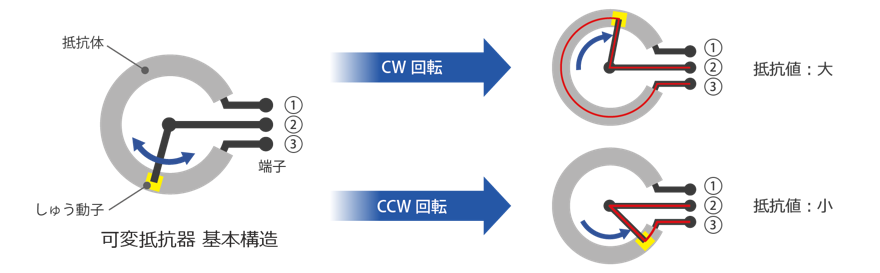
\includegraphics[scale=0.5]{/Users/ohyamasan/Downloads/TMCIT-Report/EE_Measurement/fig/pote_lp_01_02.png}
\caption{可変抵抗器の原理}
\label{fig:ALPS}
\end{figure}

\subsection{CdSセンサ\cite{dsfase}\cite{8347ty34i}\cite{B056}\cite{R300000001-I023994699-00}}
\label{CDSG}
光可変抵抗器ともいう.光電効果(photoelectric effect)である光導電性を利用し,光の強さで抵抗値が変化するCdS(硫化カドミウム)の性質を利用した電子部品.
光導電性は半導体の表面に光を当てるとキャリアが増加し,抵抗率が下がる現象である.
そのため,セルに当たる光が多ければ,抵抗値は低くなる.
赤外線や可視光線や紫外線など、広範囲の周波数にも反応するため,明るさセンサーや街の街灯のスイッチング等に用いられる.

\subsection{力センサ\cite{asdfsa}\cite{canon}}
\label{PG}
感圧センサともいう.
特殊導電部材(ゴム・フィルム)と電極で構成される.\wfig{weight}のように,接触の圧力に応じて特殊導電部材と電極の接触面積が増減することにより,抵抗値が変わる.センサ部分は円形などで,感圧エリアが決まっている.
圧力を加えていない時でも一定の抵抗値を有しており,圧力を加えると接触電極面が増加することから,抵抗値は減少する.

\begin{figure}[h]
\centering
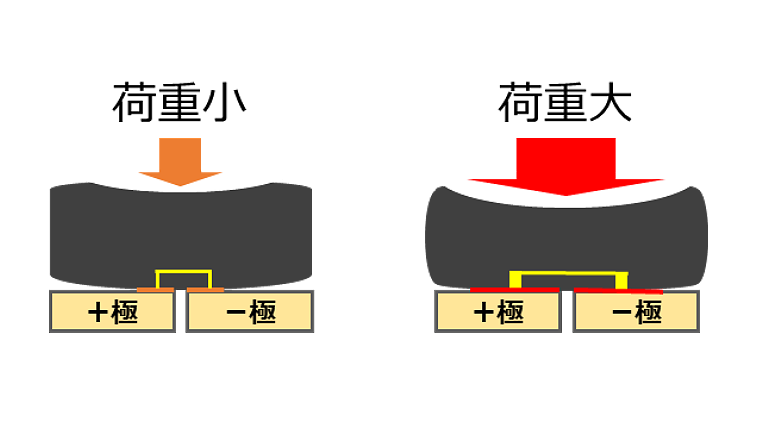
\includegraphics[scale=0.45]{/Users/ohyamasan/Downloads/TMCIT-Report/EE_Measurement/fig/sensor-03.png}
\caption{力センサの原理}
\label{fig:weight}
\end{figure}

\subsection{発光ダイオード\cite{dafadsav}\cite{gjkdgfbn}}
\label{LEDG}
LED(Light Emitting Diode)ともいう.
pn接合でできている.順方向の電圧を加えることにより,再結合エネルギーが光になって放出される.
電気エネルギーを直接光エネルギーに変換できるため,従来の光源と比べてエネルギー効率が高い.
白色LEDは\wfig{aokiro}のように,青色LED+黄色蛍光体(現在主流)のものと,\wfig{rgb}のように,赤色LED+緑色LED+青色LEDで作るものなどがある.

\begin{figure}[h]
  \begin{minipage}[]{0.5\hsize}
    \centering
    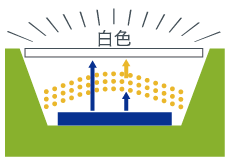
\includegraphics[scale=0.8]{/Users/ohyamasan/Downloads/TMCIT-Report/EE_Measurement/fig/led_what3_jp1.png}
    \caption{青色+黄色蛍光体手法}
    \label{fig:aokiro}
  \end{minipage}
  \begin{minipage}[]{0.5\hsize}
    \centering
    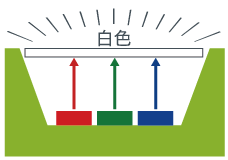
\includegraphics[scale=0.8]{/Users/ohyamasan/Downloads/TMCIT-Report/EE_Measurement/fig/led_what3_jp2.png}
    \caption{赤色+緑色+青色手法}
    \label{fig:rgb}
  \end{minipage}
\end{figure}


\subsection{真値と誤差及び相対誤差(誤差率)\cite{1130000797667922816}}
\subsubsection{真値(true value)}
真値とは,測定量(測定値ではない)が単位の何倍であるのかを示している値である.
真値は必ず存在すると仮定しても我々は真値そのものは知ることができず,ただその存在する範囲を推定することが出来るだけである.
そのため誤差は正負の符号を持っているが,それを確定することができない.
\subsubsection{誤差及び相対誤差}
測定値(measured value)及び,誤差(error)はそれぞれ,\weq{keisoku},\weq{gosa}で定義される.
\begin{align}
	測定値 &= 倍数 \times 単位\label{eq:keisoku}\\
	誤差 &= 測定値 − 真値\label{eq:gosa}
\end{align}
また,相対誤差(relative error)とは真値に対する誤差の比である.
但し真値は不明なことが多いため,通常は\weq{soutaigosa}のように誤差が小さいとして真値の代わりに測定値で割る.
\begin{eqnarray}
	相対誤差 = \frac{誤差}{真値} \fallingdotseq \frac{誤差}{測定値}
	\label{eq:soutaigosa}
\end{eqnarray}
相対誤差を百分率などで表した値を誤差率と呼ぶ.
また,以上のことから\weq{hutasikasa}のように表すこともできることがわかる\cite{1130000797042387712}.
\begin{eqnarray}
	測定値=真値 \pm 誤差=真値(1\pm 相対誤差)
\label{eq:hutasikasa}
\end{eqnarray}

\subsection{統計処理(正規分布・平均値・標準偏差)}
\subsubsection{正規分布(normal distribution)\cite{1130848328216058496}\cite{6602}}
左右対称の釣鐘型(平均値から離れるにつれて個数が減る)に値が分布している分布で,山の頂点に平均値がくる.
\wfig{normal-fig}は横軸に測定量,縦軸に正規分布の確率密度関数(probability density function)をプロットしたものである.
全体の面積(全確率)は\weq{int-nor}より1である.

\begin{figure}
\centering
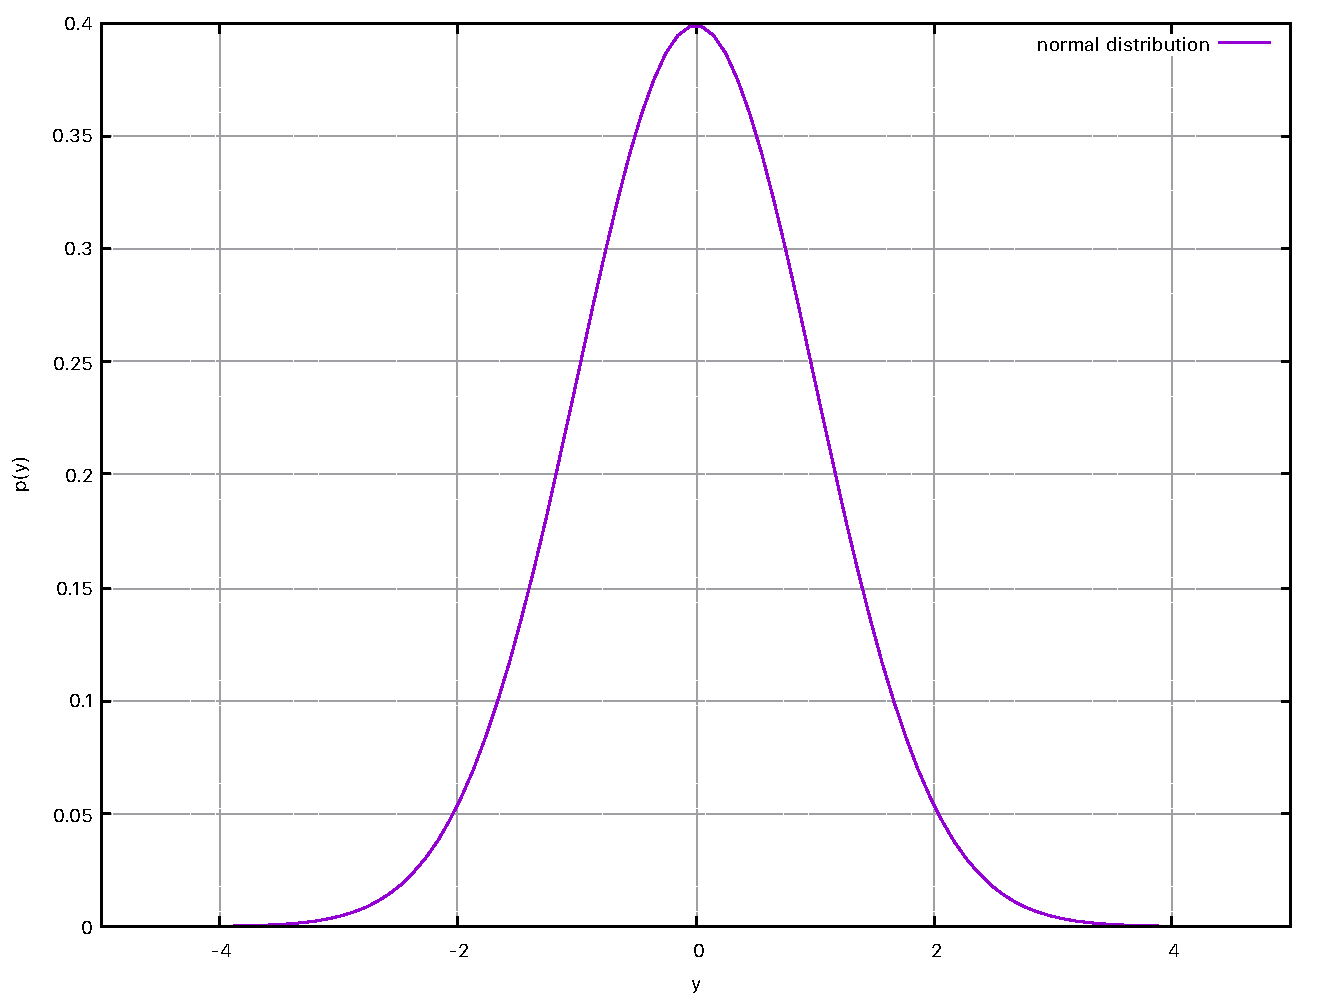
\includegraphics[scale=0.5]{/Users/ohyamasan/Downloads/TMCIT-Report/EE_Measurement/pre/plot.pdf}
\caption{正規分布}
\label{fig:normal-fig}
\end{figure}

\begin{equation}
\label{13}
p(x)=p(X=x)
\end{equation}

\begin{equation}
\label{eq:kakuritumitudo-fx}
p(x)=\frac{1}{\sqrt{2\pi}\sigma} \exp \left\{-\frac{(x-\mu)^2}{2\sigma^2}\right\}
\end{equation}

\begin{align}
\label{eq:int-nor}
\int_{-\infty}^{\infty} p(x)\,dx&=\frac{1}{\sqrt{2\pi}\sigma} \int_{-\infty}^{\infty} \exp \left(\frac{(x-\mu)^{2}}{2\sigma^{2}}\right)dx\nonumber\\
=&\frac{1}{\sqrt{2\pi}\sigma } \int_{-\infty}^{\infty} \exp \left(-\frac{y^{2}}{2\sigma^{2}}\right)dy\nonumber\\
=&\frac{1}{\sqrt{2\pi}\sigma }\sqrt{2\sigma^{2}\pi}=1
\end{align}

\subsubsection{平均値(mean)}
(算術)平均値とは$N$個全てのデータの総和を$N$個で割って得られる値で,\weq{heikinchi}で表すことができる\cite{1130848328216058496}.
\begin{equation}
	\bar{y} = \frac{1}{N}\sum^N_{i = 1}y_i
	\label{eq:heikinchi}
\end{equation}		

\subsubsection{標準偏差(standard deviation)\cite{1130000797042387712}}
標準偏差とは平均値を基準に各測定量がどれほどのばらついているかを定量的に表す値で,\weq{hyoujunhensa}で表すことができる.
\begin{equation}
	\sigma = \sqrt{\frac{1}{N - 1}\sum^N_{i = 1}(y_i - \bar{y})^2}
	\label{eq:hyoujunhensa}
\end{equation}	

\subsection{最小二乗法(method of least squares)\cite{1130848328216058496}\cite{1130282272174486912}}
2つの測定データ$y, x$間に一次方程式の関係があるとし,
\begin{equation}
	y = ax + b
	\label{eq:aiu}
\end{equation}
の傾き$a$,切片$b$を測定データからもっともらしい値にすることを考える.
その際に,
\begin{eqnarray}
	I &=& \sum\limits_{i=1}^{N} \varepsilon^2_i \nonumber\\
	&=& \sum\limits_{i=1}^{N} \bigl( y_i - f(x_i)\bigr)^2\nonumber\\\
	&=& \sum\limits_{i=1}^{N} \bigl( y_i - (ax_i+b)\bigr)^2
	\label{eq:error}
\end{eqnarray}
を最小にする$a$,$b$を求める.
これを最小二乗法といい,誤差を伴う測定値の処理においてその誤差の二乗の和を最小にすることで,最も確からしい関係式を求める方法である.前述の通り,誤差は正負あるため,2乘をしている.絶対値を用いると偏微分が不可能なため,平方根を用いた方法で行っている.
\begin{eqnarray}
	\frac{\partial}{\partial a}I(a,b) &=& 0\\
	\frac{\partial}{\partial b}I(a,b) &=& 0
\end{eqnarray}
から得られる方程式を,それぞれ$a$,$b$について解けば良く,それぞれの解を得るための方程式は次の2つを用いることになる.
\begin{equation}
	a = \frac{\sum_{n=1}^{n}(x_i -\bar{x})(y_i-\bar{y})}{\sum_{n=1}^{n}(x_i-\bar{x})^2}
	\label{eq:saisyou1}
\end{equation}
\begin{equation}
	b = \bar{y}-\frac{\sum_{n=1}^{n}(x_i -\bar{x})(y_i-\bar{y})}{\sum_{n=1}^{n}(x_i-\bar{x})^2} \bar{x}
	\label{eq:saisyou2}
\end{equation}
ここでは,\weq{aiu}のように1次式の形のものを示したが,一般に\weq{ippan}のような実験式に対して\weq{least-i}のように定義される.
\begin{align}
y&=F(x;a,b,c,\cdots)\label{eq:ippan}\\
(&xは変数,a,b,c,\cdots は定数)\nonumber
\end{align}
\begin{equation}
\label{eq:least-i}
I \equiv \sum_{i} (y_{i}-f(x_{i}))^{2} \quad \left(\frac{\partial I}{\partial a}=0 \to aを決定,\frac{\partial I}{\partial b}=0 \to bを決定 \cdots \right)
\end{equation}


\clearpage

\section{方法}
\subsection{使用器具}
今回の実験で使用した器具を
\subsection{実験手順}
\newpage
\section{結果}
\subsection{実習2-1 課題実験}
\begin{itemize}
\item プログラム\ref{ex21-block}は定電圧を100回測定するプログラムである.このようにNの数を99にすることで100回のデータ測定が可能となる.
\item 実行後,フロントパネルでは,\wfig{ex21-flont}のように表示された.
\item \wtab{GND}から\wtab{fiveV}にGND,3.3\,\rm{V},5\,\rm{V}それぞれに接続した際の出力電圧を示す.
また,\wtab{means}は計測データから算出された平均値・標準偏差である.算出方法は\weq{mean},\weq{nut},\weq{keisan-nut}の通りである\cite{7d69cf97-0c1f}.導出過程で利用したExcel関数\weq{SUM}, \weq{SQRT}はそれぞれ,$\sum_{A}^{B}$, $\sqrt{A}$に対応している.
\begin{align}
平均値\,\rm{V}&:=(SUM(X_{0}:X_{99}))/100 (=MEAN_{v})\label{eq:mean}\\
標準偏差 - 推定値\,\rm{V}&:=STDEV.S(X_{0}:X_{99})\label{eq:nut}\\
標準偏差 - 計算値\,\rm{V}&:=SQRT((X_{i}-MEAN_{v})^2/99)\label{eq:keisan-nut}\\
X_{i}&:データのi番目 \nonumber \\
MEAN_{v}&:上で計算した平均値をとる定数.GND, 3.3\,\rm{V}, 5\,\rm{V}の場合の計3種類\nonumber\\
SUM(A:B)&:AからBまでの和を返すExcel関数\label{eq:SUM}\\
STDEV.S(A:B)&:引数AからBをもとに,母集団の標準偏差の推定値を返すExcel関数\label{eq:STDEV.S}\\
SQRT(A)&:Aの平方根を返すExcel関数\label{eq:SQRT}
\end{align}
\end{itemize}

\begin{figure}[h]
\centering
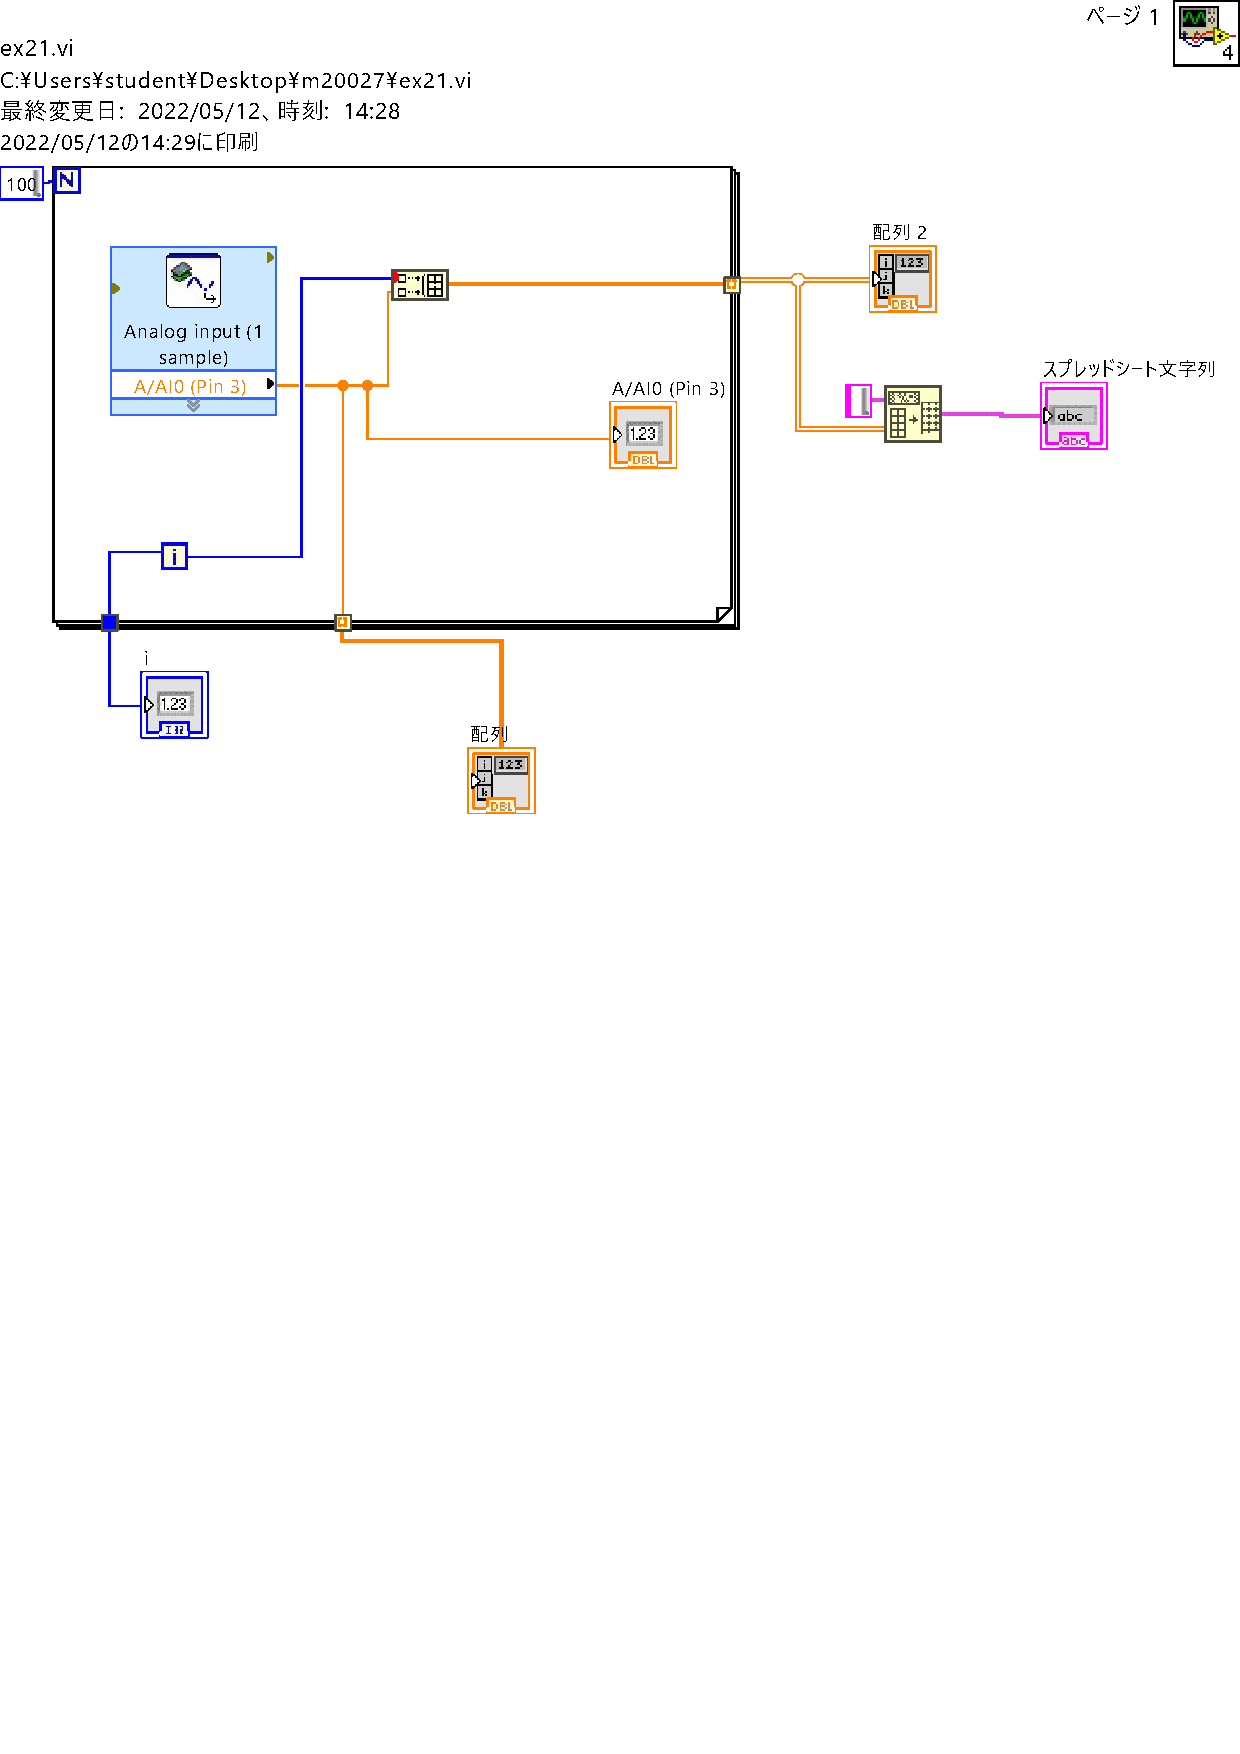
\includegraphics[scale=0.5]{./fig/ex21-block.pdf}\\
\useMycounter[\label{ex21-block}]定電圧計測のブロックダイアグラム
\end{figure}

\begin{table}[h]
\centering
\caption{Excelを用いて算出された平均値と標準偏差}
\label{tab:means}
\begin{tabular}{cccc}
\hline
    接続先 	\textbackslash 算出値 &平均値[\rm{V}] &標準偏差 - 推定値[\rm{V}]   & 標準偏差 - 計算値[\rm{V}]    \\
     \hline
  GND& 0.00636  & 0.000499  & 0.000499419 \\
3.3\,\rm{V} & 3.26256 & 0.000568 & 0.000567549 \\
 5\,\rm{V}& 4.998779 & 0.00000000000000981918 &  0.00000000000000981918 \\
\hline
\end{tabular}
\end{table}

\begin{figure}[h]
\centering
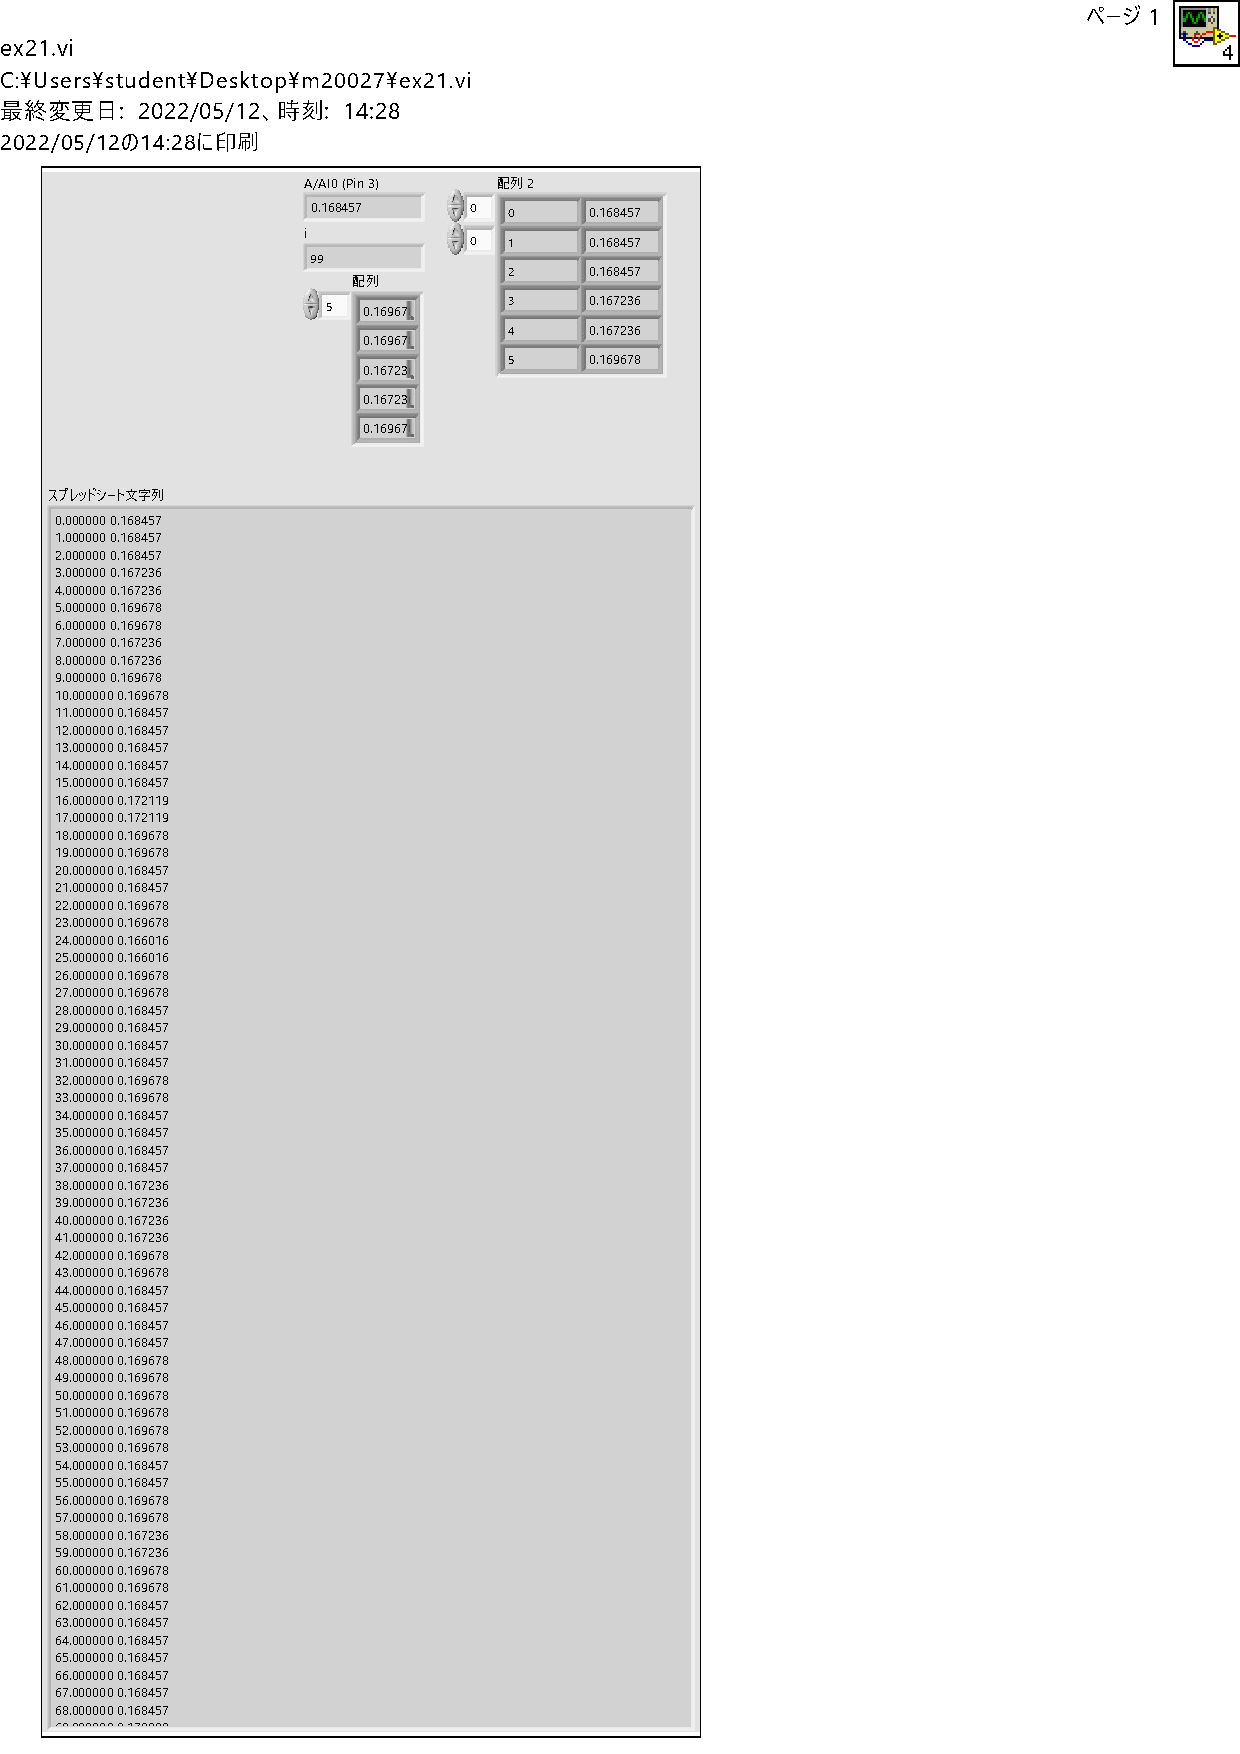
\includegraphics[scale=0.35]{./fig/ex21-flont.pdf}
\caption{定電圧計測のフロントパネル}
\label{fig:ex21-flont}
\end{figure}

\begin{table}[t]
\centering
 \caption{GND接続時の出力電圧}
 \label{tab:GND}
 \scalebox{0.7}{
\begin{tabular}{cccccccc}
\hline
測定回数[\rm{回}]&出力電圧[\rm{V}]&測定回数[\rm{回}]&出力電圧[\rm{V}]&測定回数[\rm{回}] &出力電圧[\rm{V}] &測定回数[\rm{回}] &出力電圧[\rm{V}] \\
\hline
0  & 0.006104 & 25 & 0.006104 & 50 & 0.006104 & 75 & 0.006104 \\
1  & 0.007324 & 26 & 0.007324 & 51 & 0.006104 & 76 & 0.006104 \\
2  & 0.006104 & 27 & 0.007324 & 52 & 0.006104 & 77 & 0.006104 \\
3  & 0.007324 & 28 & 0.007324 & 53 & 0.006104 & 78 & 0.006104 \\
4  & 0.007324 & 29 & 0.007324 & 54 & 0.006104 & 79 & 0.006104 \\
5  & 0.006104 & 30 & 0.007324 & 55 & 0.006104 & 80 & 0.006104 \\
6  & 0.006104 & 31 & 0.006104 & 56 & 0.006104 & 81 & 0.006104 \\
7  & 0.006104 & 32 & 0.006104 & 57 & 0.006104 & 82 & 0.007324 \\
8  & 0.006104 & 33 & 0.006104 & 58 & 0.006104 & 83 & 0.007324 \\
9  & 0.006104 & 34 & 0.006104 & 59 & 0.006104 & 84 & 0.006104 \\
10 & 0.006104 & 35 & 0.007324 & 60 & 0.006104 & 85 & 0.006104 \\
11 & 0.006104 & 36 & 0.007324 & 61 & 0.006104 & 86 & 0.007324 \\
12 & 0.006104 & 37 & 0.006104 & 62 & 0.006104 & 87 & 0.007324 \\
13 & 0.007324 & 38 & 0.006104 & 63 & 0.006104 & 88 & 0.006104 \\
14 & 0.007324 & 39 & 0.006104 & 64 & 0.006104 & 89 & 0.006104 \\
15 & 0.007324 & 40 & 0.006104 & 65 & 0.006104 & 90 & 0.006104 \\
16 & 0.006104 & 41 & 0.006104 & 66 & 0.006104 & 91 & 0.006104 \\
17 & 0.006104 & 42 & 0.006104 & 67 & 0.006104 & 92 & 0.006104 \\
18 & 0.006104 & 43 & 0.006104 & 68 & 0.006104 & 93 & 0.006104 \\
19 & 0.006104 & 44 & 0.006104 & 69 & 0.006104 & 94 & 0.006104 \\
20 & 0.006104 & 45 & 0.006104 & 70 & 0.006104 & 95 & 0.006104 \\
21 & 0.006104 & 46 & 0.006104 & 71 & 0.006104 & 96 & 0.006104 \\
22 & 0.007324 & 47 & 0.006104 & 72 & 0.006104 & 97 & 0.007324 \\
23 & 0.007324 & 48 & 0.006104 & 73 & 0.006104 & 98 & 0.007324 \\
24 & 0.006104 & 49 & 0.006104 & 74 & 0.006104 & 99 & 0.006104\\
\hline
\end{tabular}
}
 \end{table}
 
\begin{table}[b]
 \centering
 \caption{3.3\,\rm{V}接続時の出力電圧}
 \label{tab:three-threeV}
\scalebox{0.7}{
\begin{tabular}{cccccccc}
\hline
測定回数[\rm{回}]&出力電圧[\rm{V}]&測定回数[\rm{回}]&出力電圧[\rm{V}]&測定回数[\rm{回}] &出力電圧[\rm{V}] &測定回数[\rm{回}] &出力電圧[\rm{V}] \\
\hline
0  & 3.262939 & 25 & 3.262939 & 50 & 3.261718 & 75 & 3.262939 \\
1  & 3.262939 & 26 & 3.262939 & 51 & 3.262939 & 76 & 3.262939 \\
2  & 3.262939 & 27 & 3.262939 & 52 & 3.262939 & 77 & 3.262939 \\
3  & 3.262939 & 28 & 3.262939 & 53 & 3.262939 & 78 & 3.262939 \\
4  & 3.262939 & 29 & 3.262939 & 54 & 3.262939 & 79 & 3.261718 \\
5  & 3.261718 & 30 & 3.262939 & 55 & 3.262939 & 80 & 3.261718 \\
6  & 3.261718 & 31 & 3.262939 & 56 & 3.262939 & 81 & 3.262939 \\
7  & 3.262939 & 32 & 3.262939 & 57 & 3.262939 & 82 & 3.262939 \\
8  & 3.262939 & 33 & 3.262939 & 58 & 3.262939 & 83 & 3.262939 \\
9  & 3.262939 & 34 & 3.261718 & 59 & 3.262939 & 84 & 3.262939 \\
10 & 3.262939 & 35 & 3.261718 & 60 & 3.262939 & 85 & 3.261718 \\
11 & 3.262939 & 36 & 3.261718 & 61 & 3.262939 & 86 & 3.261718 \\
12 & 3.262939 & 37 & 3.261718 & 62 & 3.262939 & 87 & 3.262939 \\
13 & 3.261718 & 38 & 3.261718 & 63 & 3.262939 & 88 & 3.262939 \\
14 & 3.261718 & 39 & 3.261718 & 64 & 3.262939 & 89 & 3.262939 \\
15 & 3.261718 & 40 & 3.261718 & 65 & 3.262939 & 90 & 3.262939 \\
16 & 3.261718 & 41 & 3.262939 & 66 & 3.262939 & 91 & 3.262939 \\
17 & 3.262939 & 42 & 3.262939 & 67 & 3.262939 & 92 & 3.262939 \\
18 & 3.262939 & 43 & 3.261718 & 68 & 3.262939 & 93 & 3.262939 \\
19 & 3.262939 & 44 & 3.261718 & 69 & 3.262939 & 94 & 3.262939 \\
20 & 3.262939 & 45 & 3.261718 & 70 & 3.262939 & 95 & 3.262939 \\
21 & 3.262939 & 46 & 3.261718 & 71 & 3.261718 & 96 & 3.262939 \\
22 & 3.261718 & 47 & 3.262939 & 72 & 3.261718 & 97 & 3.262939 \\
23 & 3.261718 & 48 & 3.262939 & 73 & 3.261718 & 98 & 3.261718 \\
24 & 3.262939 & 49 & 3.261718 & 74 & 3.261718 & 99 & 3.261718 \\
\hline
\end{tabular}
}
\end{table}

\begin{table}[t]
\centering
 \caption{5\,\rm{V}接続時の出力電圧}
 \label{tab:fiveV}
 \scalebox{0.7}{
\begin{tabular}{cccccccc}
\hline
測定回数[\rm{回}]&出力電圧[\rm{V}]&測定回数[\rm{回}]&出力電圧[\rm{V}]&測定回数[\rm{回}]&出力電圧[\rm{V}]&測定回数[\rm{回}]&出力電圧[\rm{V}]\\
\hline
0  & 4.998779 & 25 & 4.998779 & 50 & 4.998779 & 75 & 4.998779 \\
1  & 4.998779 & 26 & 4.998779 & 51 & 4.998779 & 76 & 4.998779 \\
2  & 4.998779 & 27 & 4.998779 & 52 & 4.998779 & 77 & 4.998779 \\
3  & 4.998779 & 28 & 4.998779 & 53 & 4.998779 & 78 & 4.998779 \\
4  & 4.998779 & 29 & 4.998779 & 54 & 4.998779 & 79 & 4.998779 \\
5  & 4.998779 & 30 & 4.998779 & 55 & 4.998779 & 80 & 4.998779 \\
6  & 4.998779 & 31 & 4.998779 & 56 & 4.998779 & 81 & 4.998779 \\
7  & 4.998779 & 32 & 4.998779 & 57 & 4.998779 & 82 & 4.998779 \\
8  & 4.998779 & 33 & 4.998779 & 58 & 4.998779 & 83 & 4.998779 \\
9  & 4.998779 & 34 & 4.998779 & 59 & 4.998779 & 84 & 4.998779 \\
10 & 4.998779 & 35 & 4.998779 & 60 & 4.998779 & 85 & 4.998779 \\
11 & 4.998779 & 36 & 4.998779 & 61 & 4.998779 & 86 & 4.998779 \\
12 & 4.998779 & 37 & 4.998779 & 62 & 4.998779 & 87 & 4.998779 \\
13 & 4.998779 & 38 & 4.998779 & 63 & 4.998779 & 88 & 4.998779 \\
14 & 4.998779 & 39 & 4.998779 & 64 & 4.998779 & 89 & 4.998779 \\
15 & 4.998779 & 40 & 4.998779 & 65 & 4.998779 & 90 & 4.998779 \\
16 & 4.998779 & 41 & 4.998779 & 66 & 4.998779 & 91 & 4.998779 \\
17 & 4.998779 & 42 & 4.998779 & 67 & 4.998779 & 92 & 4.998779 \\
18 & 4.998779 & 43 & 4.998779 & 68 & 4.998779 & 93 & 4.998779 \\
19 & 4.998779 & 44 & 4.998779 & 69 & 4.998779 & 94 & 4.998779 \\
20 & 4.998779 & 45 & 4.998779 & 70 & 4.998779 & 95 & 4.998779 \\
21 & 4.998779 & 46 & 4.998779 & 71 & 4.998779 & 96 & 4.998779 \\
22 & 4.998779 & 47 & 4.998779 & 72 & 4.998779 & 97 & 4.998779 \\
23 & 4.998779 & 48 & 4.998779 & 73 & 4.998779 & 98 & 4.998779 \\
24 & 4.998779 & 49 & 4.998779 & 74 & 4.998779 & 99 & 4.998779\\
\hline
\end{tabular}
}
\end{table}

\clearpage
\subsection{実習2-2 課題実験}
\begin{itemize}
	\item プログラム\ref{ex22-block}は変電圧測定プログラムである.これのようにNの値を11に,カウンタ変数を2で除することで0\,\rm{V}から5\,\rm{V}まで0.5\,\rm{V}刻みで出力電圧を計測することが可能となる.
	\item 実行した後のフロントパネルを\wfig{ex22-flont}に示す.また,\weq{soutaigosa}に基づいて計算した相対誤差を\wtab{fivegosa}に示す.
表からもわかるように0\,\rm{V}の際の相対誤差が飛び抜けて大きいことが読み取れる.	
	\item Excel を用いて計算したRMSEを\wtab{RMSE}に示す\cite{lm-evaluation}.
	\item RMSEの計算式は\weq{lm-evaluation},Excelでは\weq{eRMSE}で計算した.
\end{itemize}

\begin{align}
RMSE&=\sqrt{\frac{1}{n}\sum_{i=1}^{n}(y_{i}-\hat{y_{i}})^{2}}\label{eq:lm-evaluation}\\
y_{i}:観測値(n個)\quad&\qquad\hat{y_{i}}:計算値(n個)\nonumber\\
RMSE&=SQRT(1/11)*SQRT(SUM(\overline{X_{i}}^{2}))\label{eq:eRMSE}\\
\overline{X_{i}}&:X_{i}での差(誤差)\nonumber
\end{align}

\begin{figure}[h]
\centering
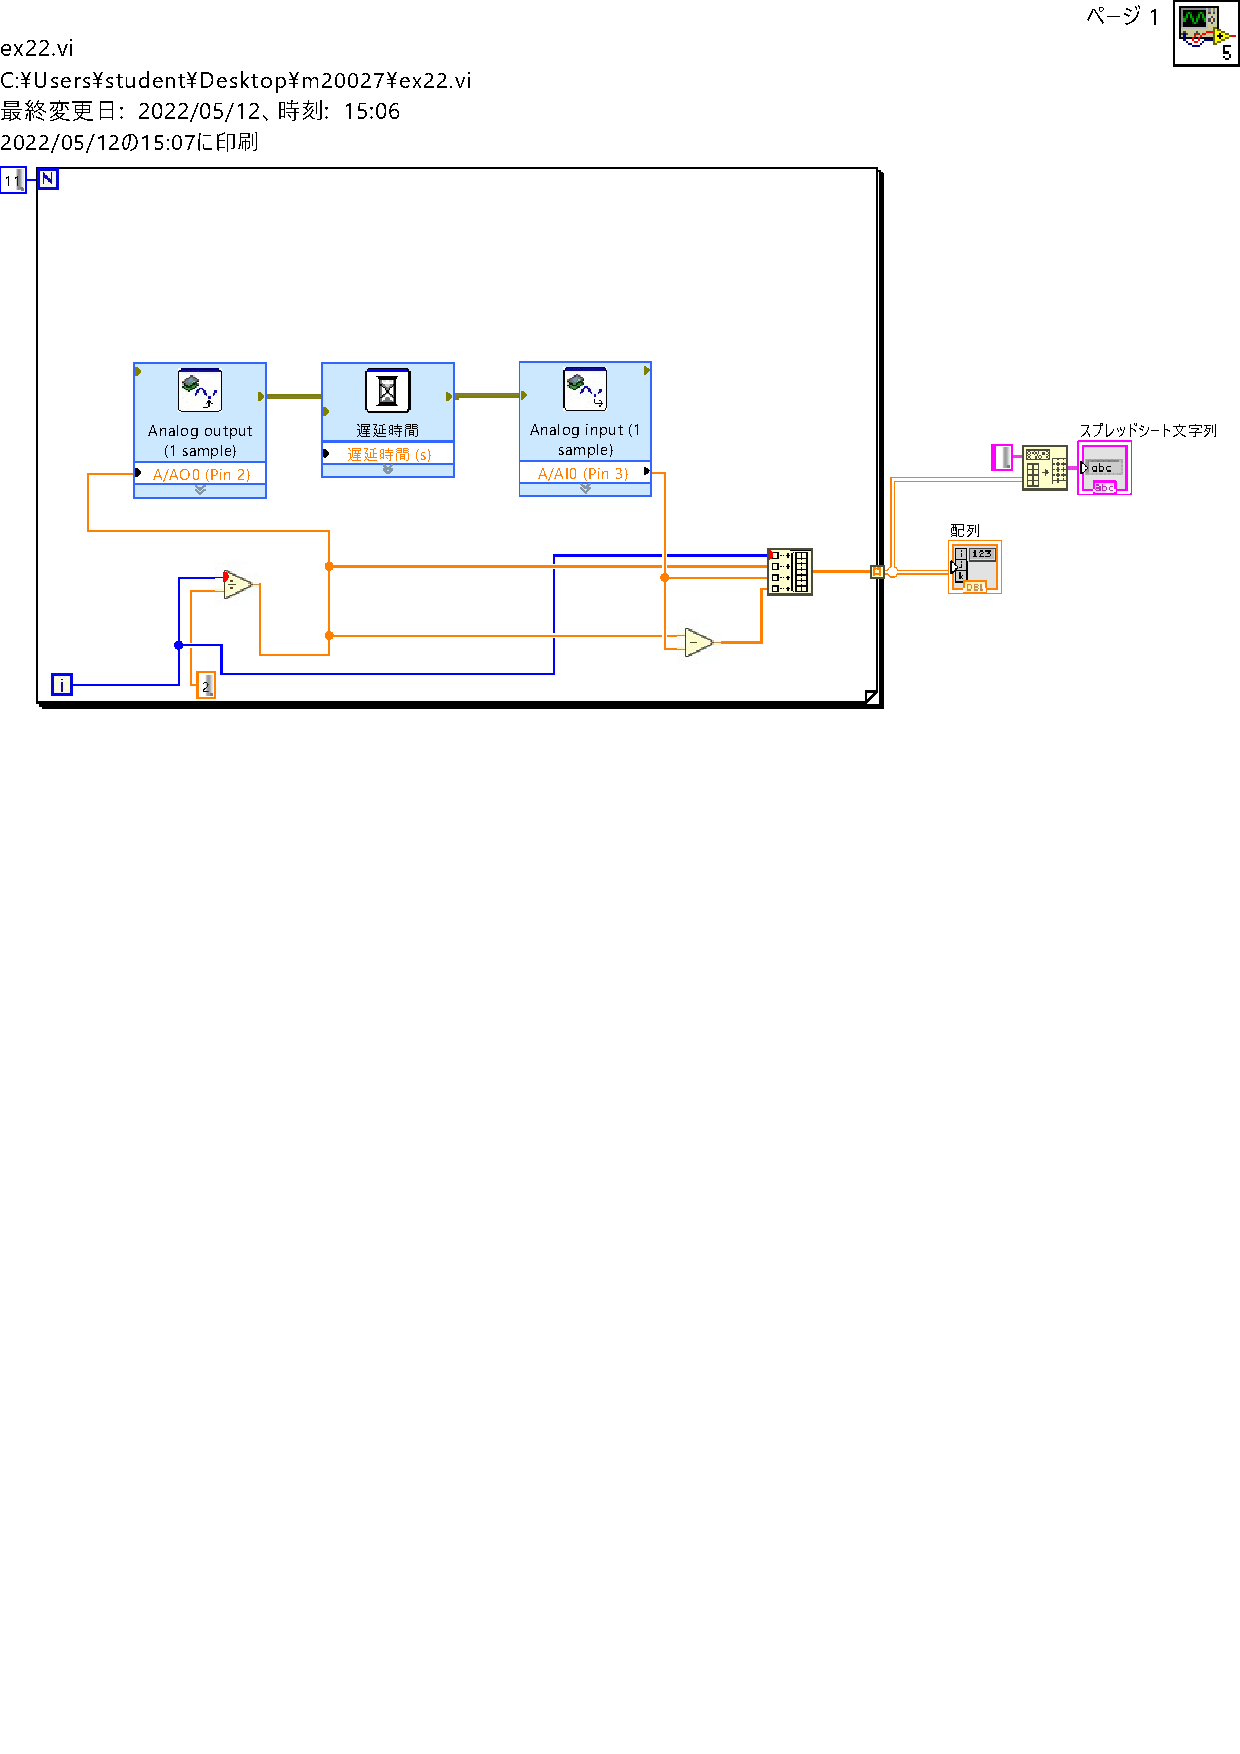
\includegraphics[scale=0.5]{./fig/ex22-block.pdf}\\
\useMycounter[\label{ex22-block}]出力電圧変化測定時のブロックダイアグラム
\end{figure}
\begin{figure}[h]
\centering
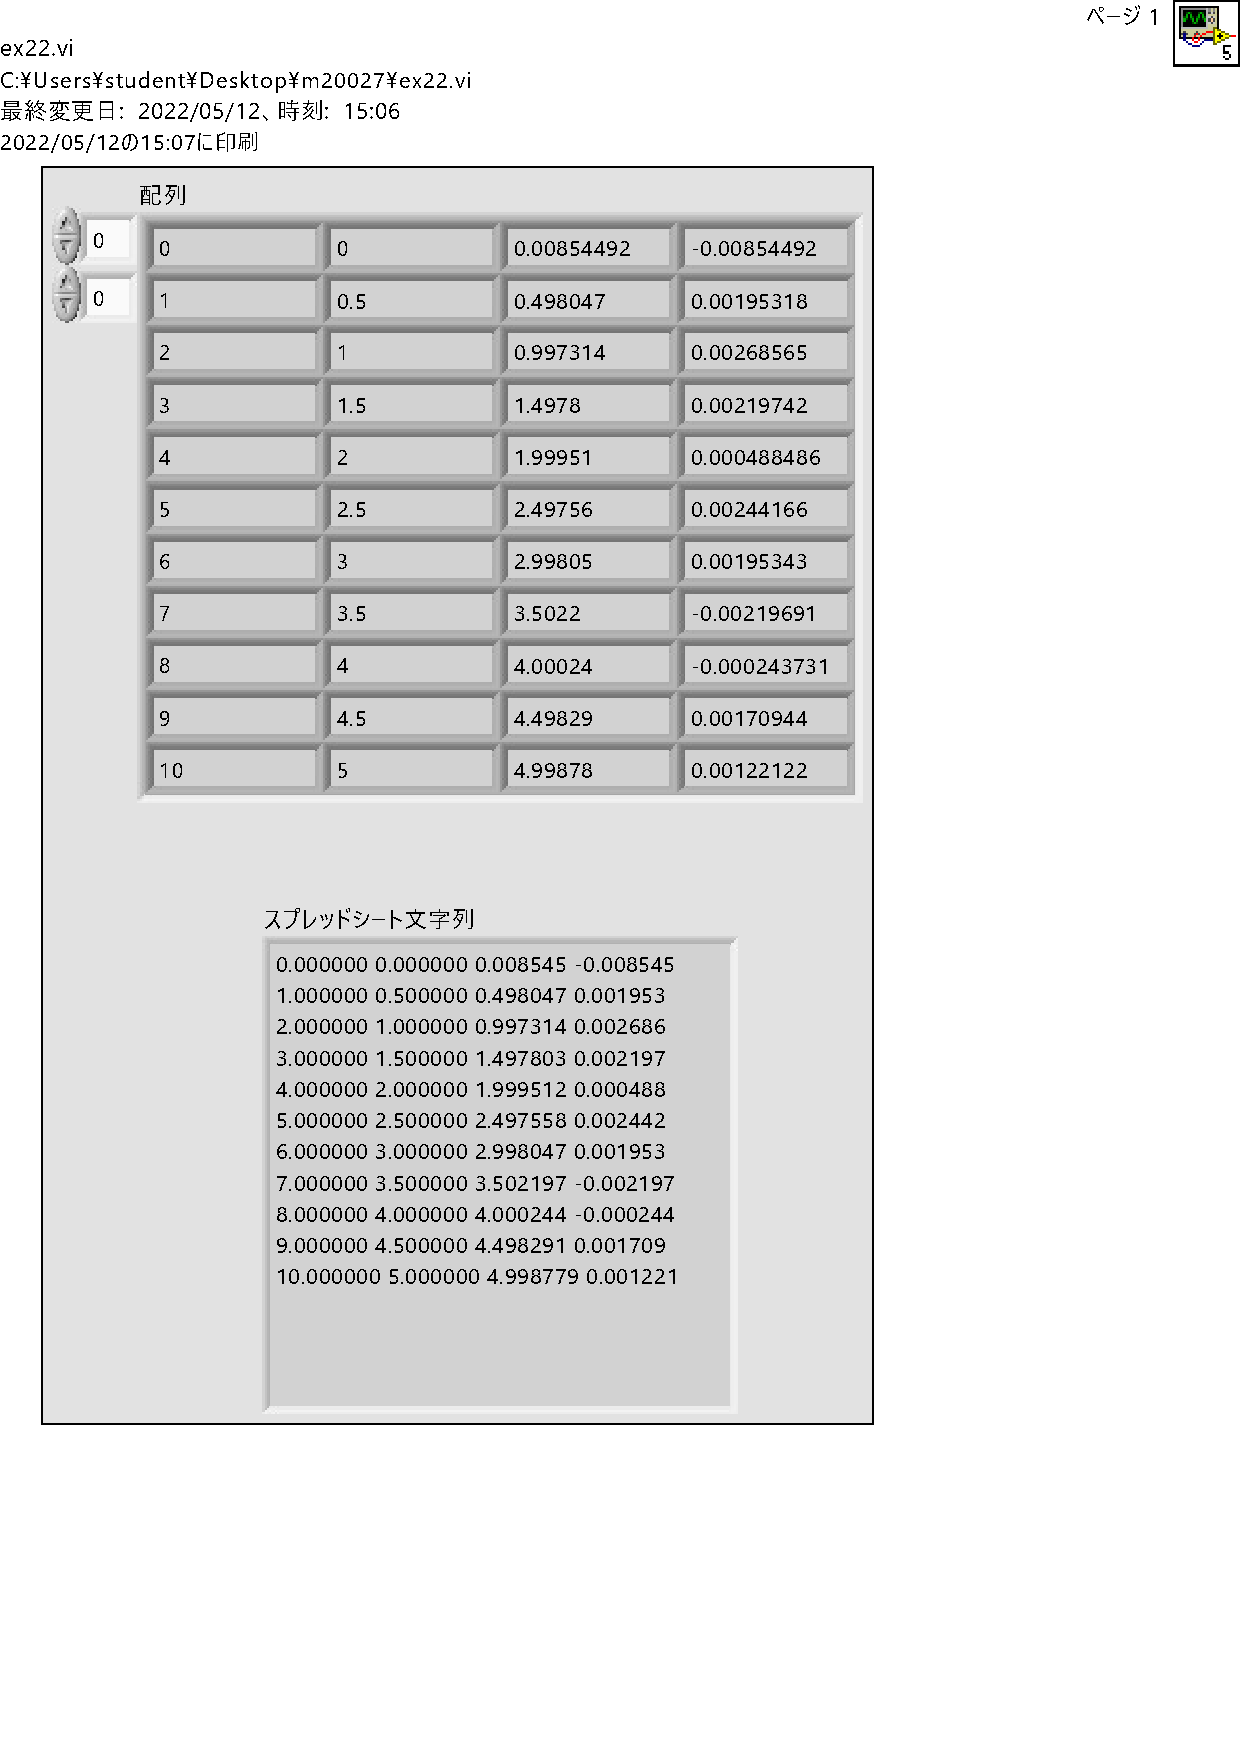
\includegraphics[scale=0.5]{./fig/ex22-flont.pdf}
\caption{出力電圧変化測定時のフロントパネル}
\label{fig:ex22-flont}
\end{figure}

\begin{table}[h]
\begin{minipage}[c]{0.5\hsize}
\centering
\caption{電圧変化測定時の相対誤差}
\label{tab:fivegosa}
\begin{tabular}{cc}
\hline
電圧[\rm{V}]  & 相対誤差[\rm{V}]\\
\hline
0   & 0  \\
0.5 & 0  \\
1   & -1 \\
1.5 & -1 \\
2   & -2 \\
2.5 & -3 \\
3   & -3 \\
3.5 & -3 \\
4   & -4 \\
4.5 & -4 \\
5   & -5 \\
\hline
\end{tabular}
\end{minipage}
\begin{minipage}[c]{0.5\hsize}
\centering
\caption{電圧変化測定時のRMSE}
\label{tab:RMSE}
\begin{tabular}{cc}
\hline
電圧[\rm{V}]  & 二乗平均平方根誤差[\rm{V}]  \\
\hline
0   & 0.002576414 \\
0.5 & 0.000956997 \\
1   & 0.000809859 \\
1.5 & 0.001030566 \\
2   & 0.000515283 \\
2.5 & 0.000367844 \\
3   & 0.000221008 \\
3.5 & 0.0000735688 \\
4   & 0.000441413 \\
4.5 & 0.000147439 \\
5   & 0.000368145\\
\hline
\end{tabular}
\end{minipage}
\end{table}
\clearpage
\subsection{実習3-1 固定抵抗の電圧電流特性}
\begin{itemize}
	\item プログラム\ref{ex31-block}は$R_{0}$の場合の,固定抵抗の電圧電流特性(0-5\,\rm{V}まで0.1\,\rm{V}刻み)を計測するプログラムである.
	\item 上図の中心部分の100という数字は$R_{0}$の値にするとよい.
	\item 実行後,フロントパネルは\wfig{ex31-flont}のようになり,計測結果は\wtab{R}のようになった.
	\item 計測データを基に作成した電圧電流特性のグラフは\wfig{3-1}である.
\end{itemize}

\begin{figure}[h]
\centering
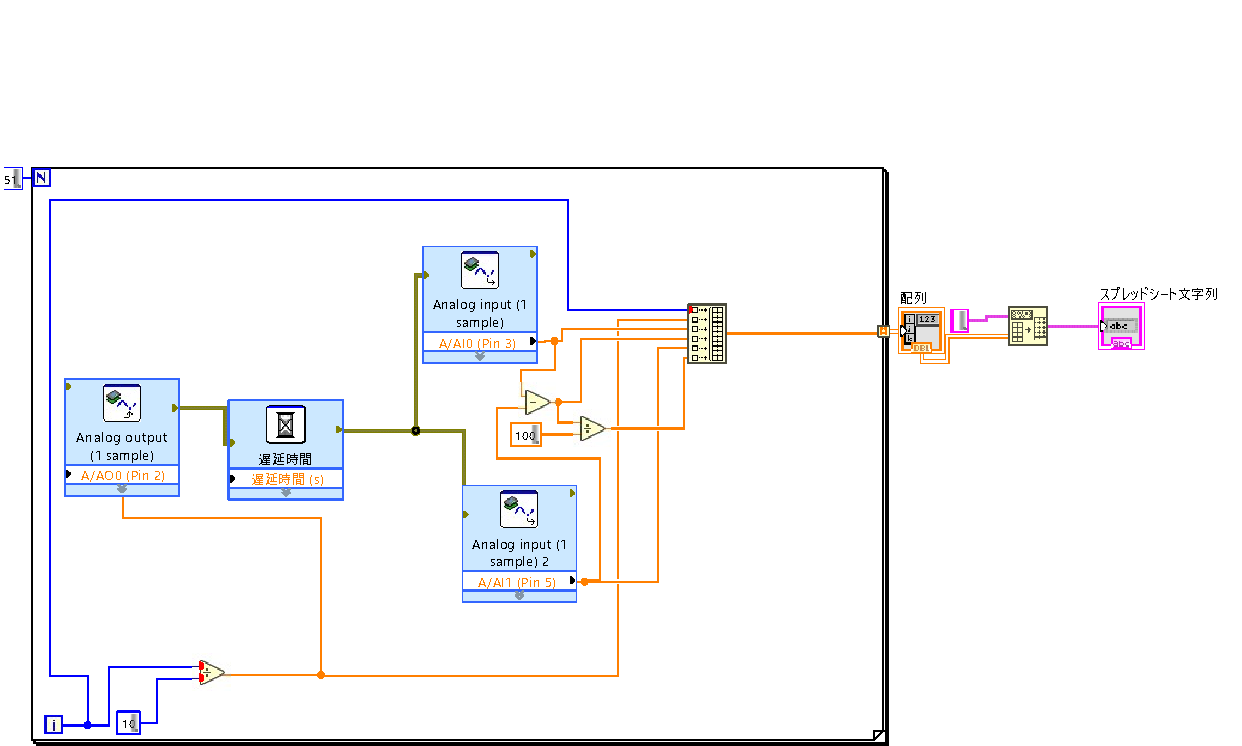
\includegraphics[scale=0.5]{./fig/ex31-block.pdf}\\
\useMycounter[\label{ex31-block}]固定抵抗の電圧電流特性計測時のブロックダイアグラム
\end{figure}
\begin{figure}[h]
\centering
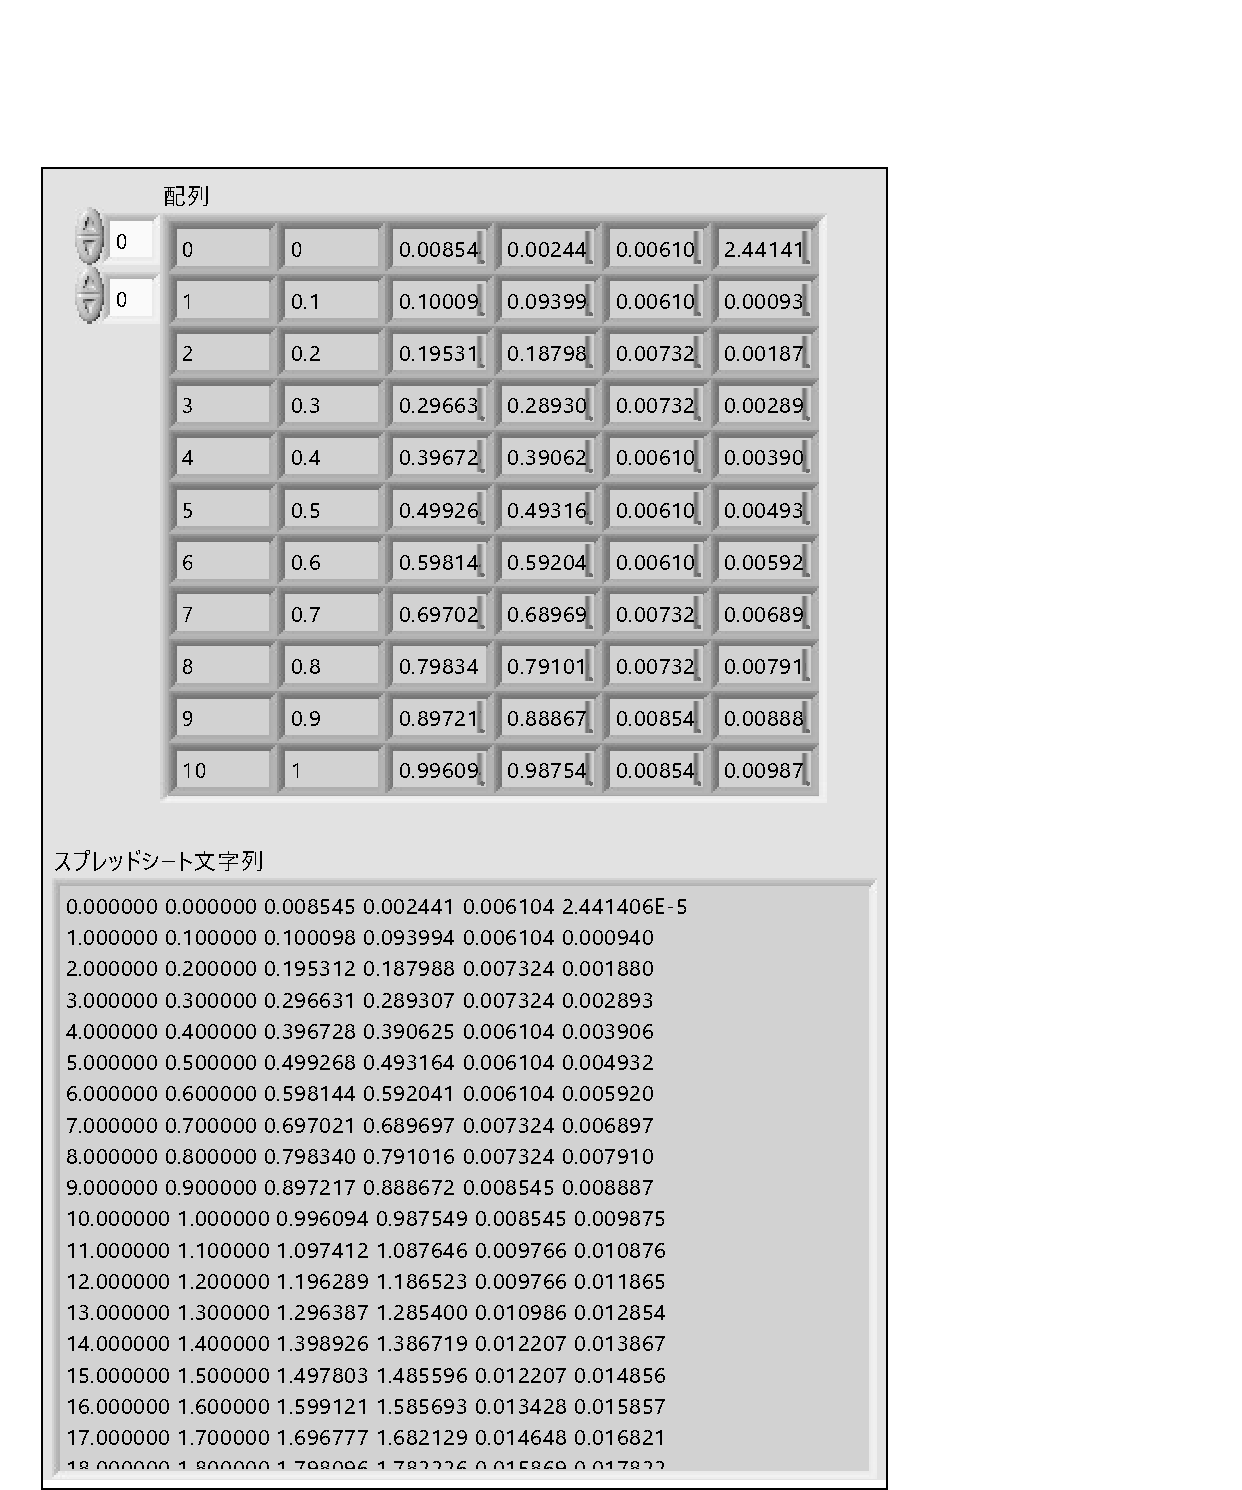
\includegraphics[scale=0.5]{./fig/ex31-flont.pdf}
\caption{固定抵抗の電圧電流特性測定時のフロントパネル}
\label{fig:ex31-flont}
\end{figure}

\begin{table}[h]
    \centering
     \caption{固定抵抗の諸特性値}    
     \label{tab:R}
     \scalebox{0.8}{
    \begin{tabular}{cccccc}
\hline
カウンタ変数 & 出力電圧[\rm{V}] & 全電圧[\rm{V}]  & $V_{R0}$[\rm{V}]   & $V_{U}$[\rm{V}]    & $I_{U}$[\rm{A}]  \\
\hline
  0      & 0    & 0.007324 & 0        & 0.007324 & 0        \\
  1      & 0.1  & 0.096436 & 0.007324 & 0.089111 & 0.0000732 \\
  2      & 0.2  & 0.197754 & 0.019531 & 0.178223 & 0.000195 \\
  3      & 0.3  & 0.297852 & 0.026855 & 0.270996 & 0.000269 \\
  4      & 0.4  & 0.39917  & 0.037842 & 0.361328 & 0.000378 \\
  5      & 0.5  & 0.498047 & 0.046387 & 0.45166  & 0.000464 \\
  6      & 0.6  & 0.595703 & 0.05249  & 0.543213 & 0.000525 \\
  7      & 0.7  & 0.697021 & 0.063477 & 0.633545 & 0.000635 \\
  8      & 0.8  & 0.797119 & 0.073242 & 0.723877 & 0.000732 \\
  9      & 0.9  & 0.897217 & 0.084229 & 0.812988 & 0.000842 \\
  10     & 1    & 0.996094 & 0.091553 & 0.904541 & 0.000916 \\
  11     & 1.1  & 1.096191 & 0.101318 & 0.994873 & 0.001013 \\
  12     & 1.2  & 1.195068 & 0.108643 & 1.086426 & 0.001086 \\
  13     & 1.3  & 1.297607 & 0.12207  & 1.175537 & 0.001221 \\
  14     & 1.4  & 1.396484 & 0.128174 & 1.26831  & 0.001282 \\
  15     & 1.5  & 1.496582 & 0.13916  & 1.357422 & 0.001392 \\
  16     & 1.6  & 1.5979   & 0.150146 & 1.447754 & 0.001501 \\
  17     & 1.7  & 1.696777 & 0.157471 & 1.539306 & 0.001575 \\
  18     & 1.8  & 1.795654 & 0.164795 & 1.630859 & 0.001648 \\
  19     & 1.9  & 1.895752 & 0.174561 & 1.721191 & 0.001746 \\
  20     & 2    & 1.994629 & 0.183105 & 1.811523 & 0.001831 \\
  21     & 2.1  & 2.094726 & 0.192871 & 1.901855 & 0.001929 \\
  22     & 2.2  & 2.194824 & 0.202637 & 1.992187 & 0.002026 \\
  23     & 2.3  & 2.294922 & 0.211182 & 2.08374  & 0.002112 \\
  24     & 2.4  & 2.395019 & 0.220947 & 2.174072 & 0.002209 \\
  25     & 2.5  & 2.495117 & 0.230713 & 2.264404 & 0.002307 \\
  26     & 2.6  & 2.593994 & 0.238037 & 2.355957 & 0.00238  \\
  27     & 2.7  & 2.694092 & 0.247803 & 2.446289 & 0.002478 \\
  28     & 2.8  & 2.794189 & 0.257568 & 2.536621 & 0.002576 \\
  29     & 2.9  & 2.894287 & 0.266113 & 2.628174 & 0.002661 \\
  30     & 3    & 2.995605 & 0.2771   & 2.718506 & 0.002771 \\
  31     & 3.1  & 3.094482 & 0.285645 & 2.808838 & 0.002856 \\
  32     & 3.2  & 3.193359 & 0.29541  & 2.897949 & 0.002954 \\
  33     & 3.3  & 3.293457 & 0.302734 & 2.990722 & 0.003027 \\
  34     & 3.4  & 3.393554 & 0.3125   & 3.081054 & 0.003125 \\
  35     & 3.5  & 3.492431 & 0.321045 & 3.171386 & 0.00321  \\
  36     & 3.6  & 3.59497  & 0.333252 & 3.261718 & 0.003333 \\
  37     & 3.7  & 3.693847 & 0.339355 & 3.354492 & 0.003394 \\
  38     & 3.8  & 3.793945 & 0.349121 & 3.444824 & 0.003491 \\
  39     & 3.9  & 3.894043 & 0.358887 & 3.535156 & 0.003589 \\
  40     & 4    & 3.99292  & 0.367432 & 3.625488 & 0.003674 \\
  41     & 4.1  & 4.091796 & 0.374756 & 3.717041 & 0.003748 \\
  42     & 4.2  & 4.193115 & 0.385742 & 3.807373 & 0.003857 \\
  43     & 4.3  & 4.274902 & 0.390625 & 3.884277 & 0.003906 \\
  44     & 4.4  & 4.272461 & 0.391846 & 3.880615 & 0.003918 \\
  45     & 4.5  & 4.270019 & 0.390625 & 3.879394 & 0.003906 \\
  46     & 4.6  & 4.268798 & 0.390625 & 3.878173 & 0.003906 \\
  47     & 4.7  & 4.266357 & 0.390625 & 3.875732 & 0.003906 \\
  48     & 4.8  & 4.266357 & 0.391846 & 3.874511 & 0.003918 \\
  49     & 4.9  & 4.263916 & 0.390625 & 3.873291 & 0.003906 \\
  50     & 5    & 4.262695 & 0.389404 & 3.873291 & 0.003894 \\
\hline
\end{tabular}
}
\end{table}

\begin{figure}[h]
        \centering
        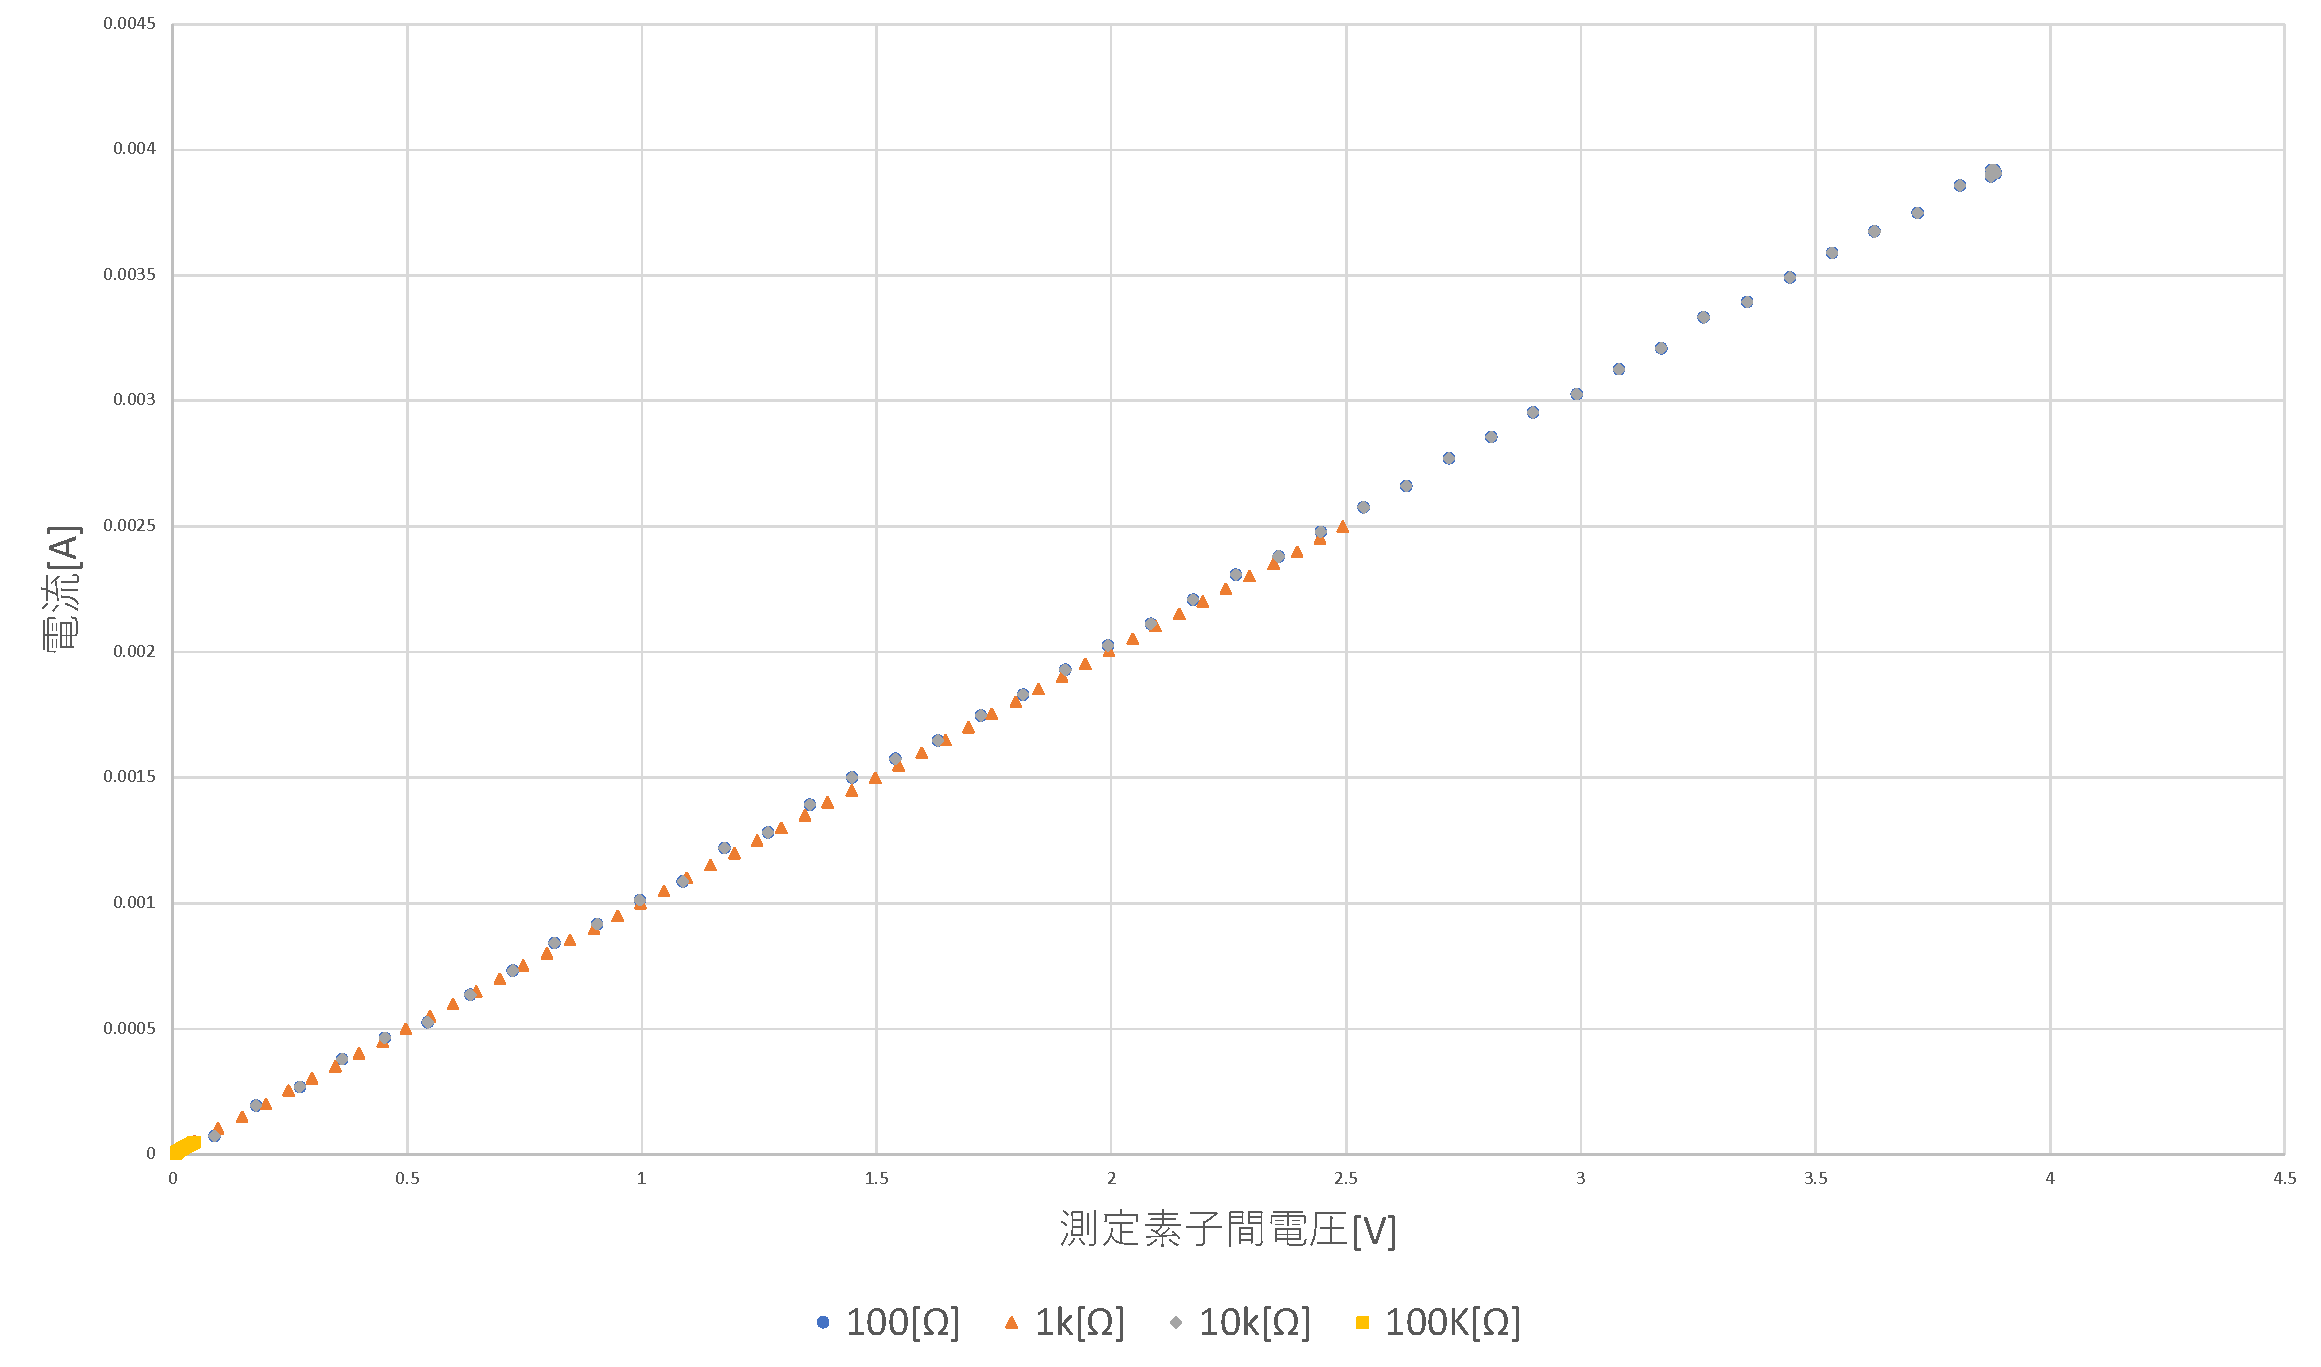
\includegraphics[scale=0.45]{./fig/3-1.pdf}
	\caption{固定抵抗の電圧電流特性}
	\label{fig:3-1}  
\end{figure}
\clearpage
\subsection{実習3-2 可変抵抗(ポテンショメータ)の電圧電流特性}
\begin{itemize}
	\item プログラム\ref{ex32-block}は可変抵抗端子1-2間の電圧電流特性を計測するプログラムである.
	\item 全ての場合において,$R_{0}$の値は10\,k\rm{$\Omega$}とした.
	\item 実行後,フロントパネルは\wfig{ex32-flont}のようになり,計測結果は\wtab{ER1-2}のようになった.
	\item 計測データを基に作成した電圧電流特性のグラフは\wfig{3-2-1}である.
	\item 端子2-3間では,\wtab{ER2-3},\wfig{3-2-2}.端子3-1間では,\wtab{ER3-1},\wfig{3-2-3}となった.
\end{itemize}

\begin{figure}[h]
\centering
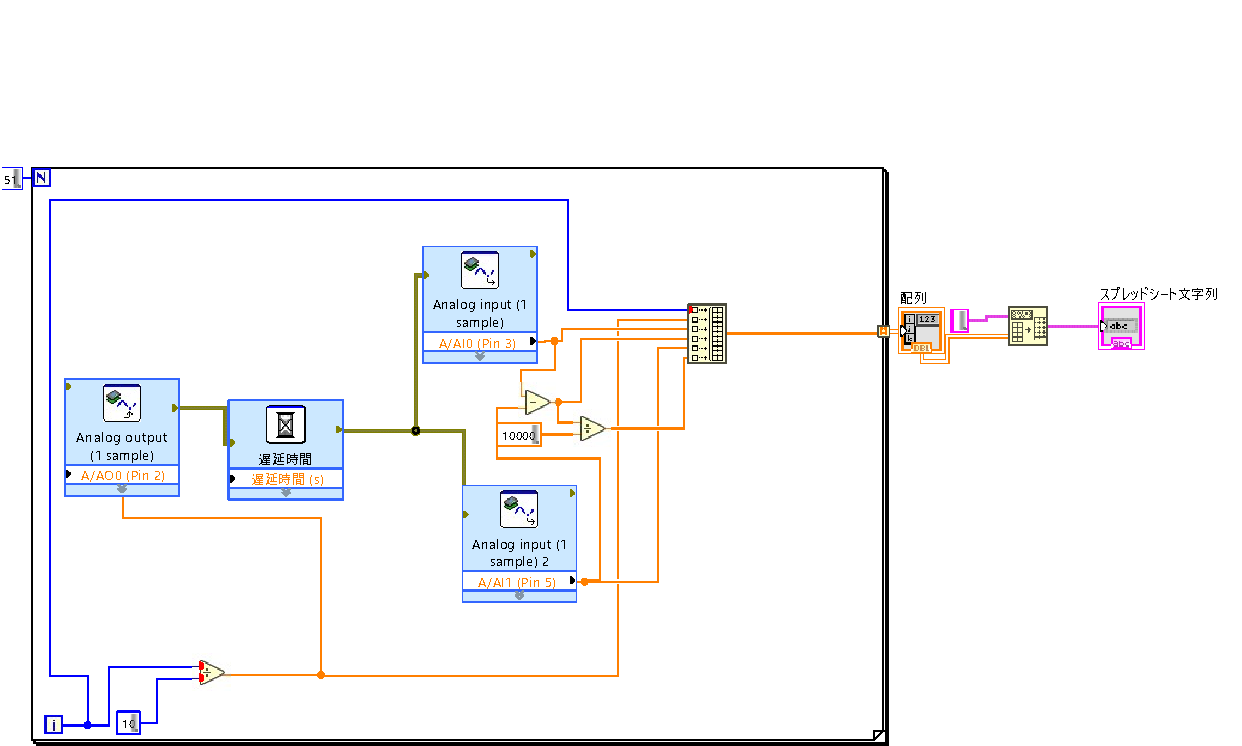
\includegraphics[scale=0.5]{./fig/ex32-block.pdf}\\
\useMycounter[\label{ex32-block}]可変抵抗の電圧電流特性計測時のブロックダイアグラム
\end{figure}

\begin{figure}[h]
\centering
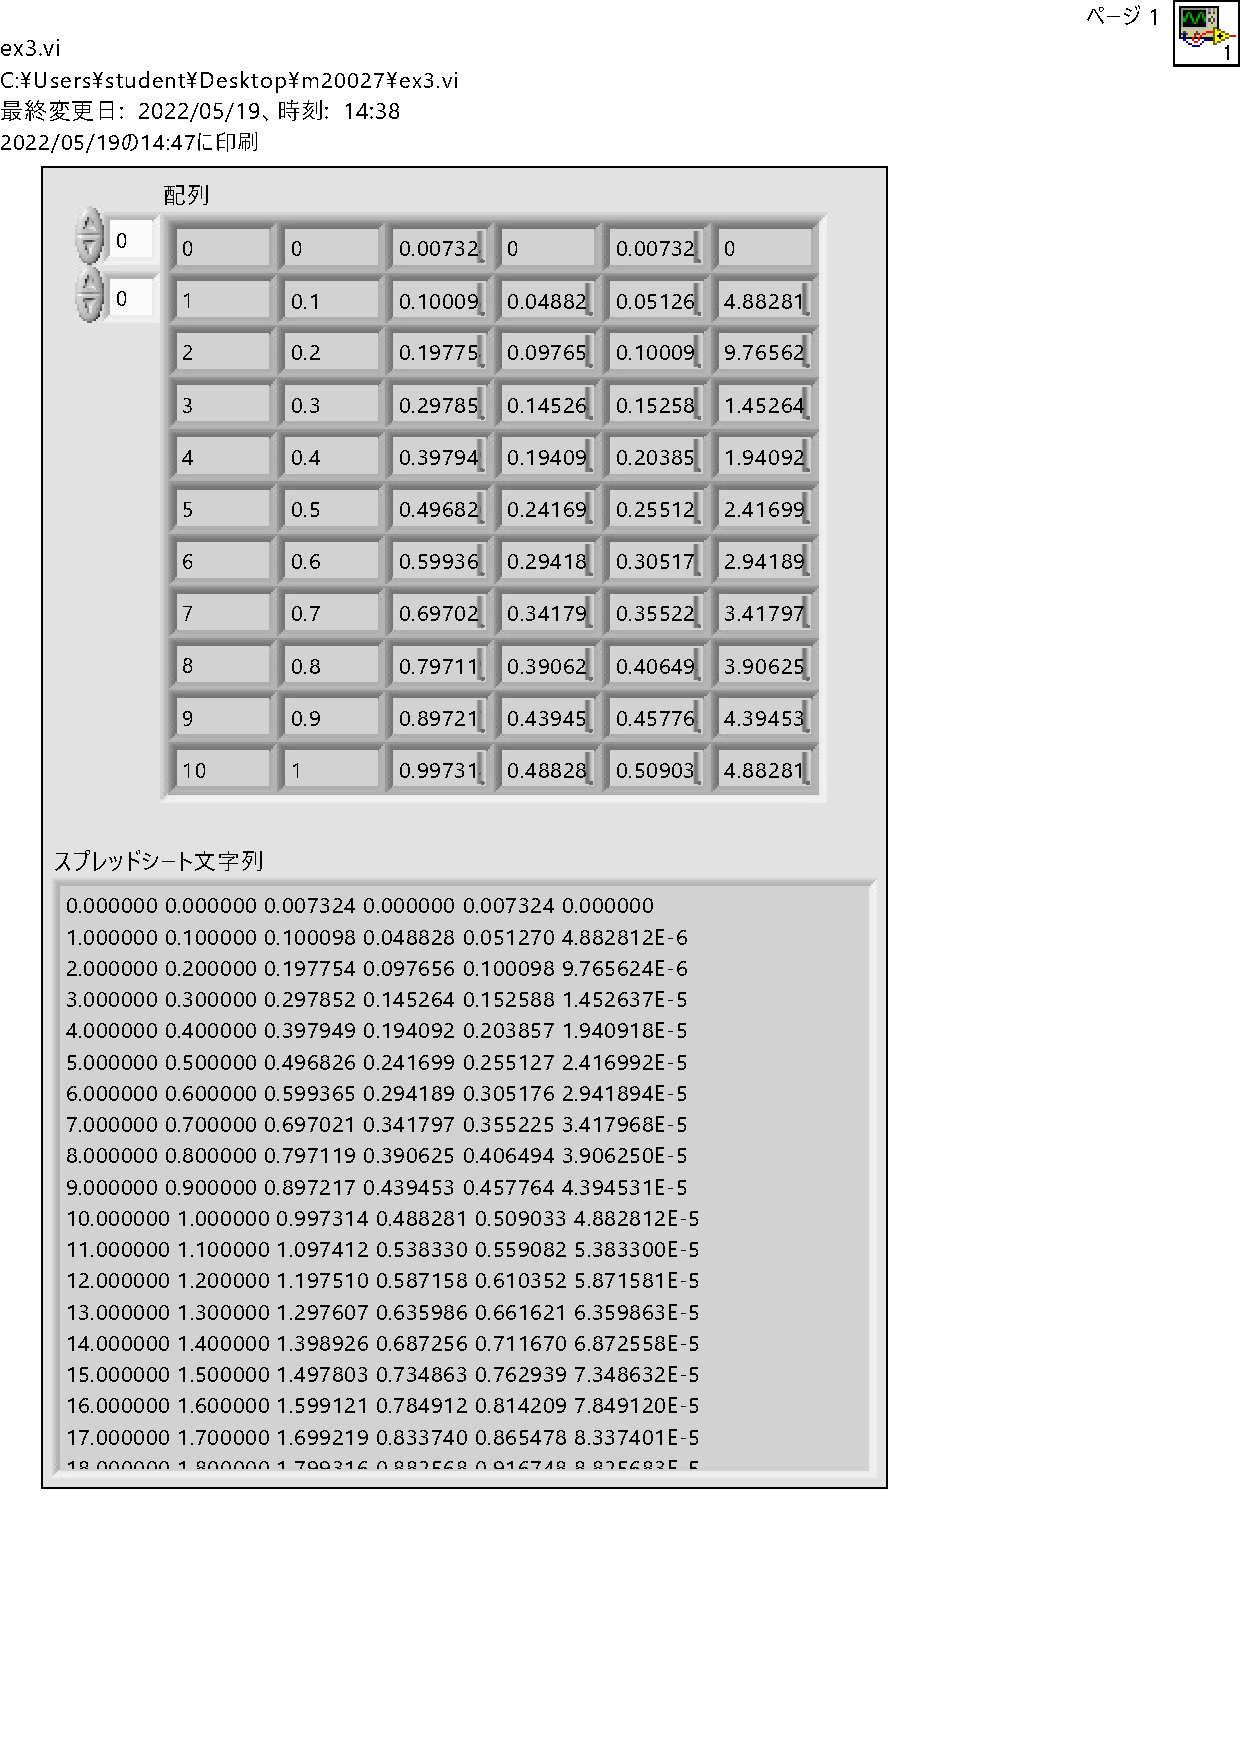
\includegraphics[scale=0.5]{./fig/ex32-flont.pdf}
\caption{可変抵抗の電圧電流特性測定時のフロントパネル}
\label{fig:ex32-flont}
\end{figure}

\begin{table}[h]
\centering
\caption{可変抵抗器(1-2端子間)の諸特性値}
\label{tab:ER1-2}
\scalebox{0.8}{
\begin{tabular}{ccccccc}
\hline
カウンタ変数 & Aでの$V_{U}$[\rm{V}] & Aでの$I_{U}$[\rm{A}] & Bでの$V_{U}$[\rm{V}]    & Bでの$I_{U}$[\rm{A}]   & Cでの$V_{U}$[\rm{V}]& Cでの$I_{U}$[\rm{A}] \\
\hline
  0      & 0.007324 & 0.00000012 & 0.006104 & 0.00000024 & 0.006104 & 0.00000024 \\
  1      & 0.048828 & 0.00000513 & 0.031738 & 0.00000696 & 0.007324 & 0.00000903 \\
  2      & 0.098877 & 0.00000977 & 0.065918 & 0.00001306 & 0.006104 & 0.00001892 \\
  3      & 0.151367 & 0.00001453 & 0.100098 & 0.00001953 & 0.006104 & 0.00002930 \\
  4      & 0.203857 & 0.00001929 & 0.133057 & 0.00002637 & 0.006104 & 0.00003894 \\
  5      & 0.253906 & 0.00002441 & 0.168457 & 0.00003296 & 0.006104 & 0.00004932 \\
  6      & 0.305176 & 0.00002930 & 0.201416 & 0.00003979 & 0.007324 & 0.00005920 \\
  7      & 0.355225 & 0.00003418 & 0.234375 & 0.00004639 & 0.007324 & 0.00006897 \\
  8      & 0.406494 & 0.00003918 & 0.268555 & 0.00005286 & 0.007324 & 0.00007910 \\
  9      & 0.456543 & 0.00004407 & 0.301514 & 0.00005957 & 0.007324 & 0.00008911 \\
  10     & 0.507812 & 0.00004907 & 0.336914 & 0.00006616 & 0.007324 & 0.00009888 \\
  11     & 0.559082 & 0.00005396 & 0.369873 & 0.00007275 & 0.006104 & 0.00010900 \\
  12     & 0.610352 & 0.00005859 & 0.404053 & 0.00007947 & 0.006104 & 0.00011900 \\
  13     & 0.661621 & 0.00006360 & 0.438232 & 0.00008606 & 0.006104 & 0.00012900 \\
  14     & 0.712891 & 0.00006848 & 0.472412 & 0.00009253 & 0.006104 & 0.00013900 \\
  15     & 0.762939 & 0.00007349 & 0.505371 & 0.00009924 & 0.006104 & 0.00014900 \\
  16     & 0.814209 & 0.00007849 & 0.539551 & 0.00010600 & 0.006104 & 0.00015900 \\
  17     & 0.865478 & 0.00008350 & 0.57251  & 0.00011300 & 0.007324 & 0.00016900 \\
  18     & 0.915527 & 0.00008838 & 0.606689 & 0.00011900 & 0.007324 & 0.00017900 \\
  19     & 0.966797 & 0.00009302 & 0.640869 & 0.00012600 & 0.007324 & 0.00018900 \\
  20     & 1.018066 & 0.00009790 & 0.673828 & 0.00013200 & 0.007324 & 0.00019900 \\
  21     & 1.068115 & 0.00010300 & 0.709228 & 0.00013900 & 0.007324 & 0.00020900 \\
  22     & 1.119385 & 0.00010800 & 0.742187 & 0.00014600 & 0.008545 & 0.00021900 \\
  23     & 1.170654 & 0.00011300 & 0.775146 & 0.00015200 & 0.008545 & 0.00022900 \\
  24     & 1.221924 & 0.00011800 & 0.809326 & 0.00015900 & 0.008545 & 0.00023900 \\
  25     & 1.273193 & 0.00012200 & 0.843506 & 0.00016600 & 0.008545 & 0.00024900 \\
  26     & 1.324463 & 0.00012700 & 0.877685 & 0.00017200 & 0.008545 & 0.00025900 \\
  27     & 1.374512 & 0.00013200 & 0.910644 & 0.00017900 & 0.009766 & 0.00026900 \\
  28     & 1.425781 & 0.00013700 & 0.944824 & 0.00018600 & 0.009766 & 0.00027900 \\
  29     & 1.477051 & 0.00014200 & 0.979004 & 0.00019200 & 0.008545 & 0.00028900 \\
  30     & 1.527099 & 0.00014700 & 1.013183 & 0.00019900 & 0.009766 & 0.00029900 \\
  31     & 1.57959  & 0.00015200 & 1.046142 & 0.00020500 & 0.010986 & 0.00030900 \\
  32     & 1.630859 & 0.00015700 & 1.080322 & 0.00021200 & 0.012207 & 0.00031900 \\
  33     & 1.680908 & 0.00016200 & 1.114502 & 0.00021900 & 0.010986 & 0.00032900 \\
  34     & 1.730957 & 0.00016700 & 1.147461 & 0.00022500 & 0.013428 & 0.00033900 \\
  35     & 1.782226 & 0.00017200 & 1.181641 & 0.00023200 & 0.012207 & 0.00034900 \\
  36     & 1.834717 & 0.00017600 & 1.21582  & 0.00023800 & 0.013428 & 0.00035900 \\
  37     & 1.885986 & 0.00018100 & 1.25     & 0.00024500 & 0.013428 & 0.00036900 \\
  38     & 1.936035 & 0.00018600 & 1.28418  & 0.00025200 & 0.014648 & 0.00037900 \\
  39     & 1.987304 & 0.00019100 & 1.317139 & 0.00025800 & 0.014648 & 0.00038900 \\
  40     & 2.038574 & 0.00019600 & 1.351318 & 0.00026500 & 0.014648 & 0.00039800 \\
  41     & 2.089844 & 0.00020100 & 1.385498 & 0.00027200 & 0.015869 & 0.00040800 \\
  42     & 2.141113 & 0.00020600 & 1.419678 & 0.00027800 & 0.015869 & 0.00041800 \\
  43     & 2.192383 & 0.00021100 & 1.453857 & 0.00028500 & 0.015869 & 0.00042800 \\
  44     & 2.241211 & 0.00021600 & 1.486816 & 0.00029100 & 0.015869 & 0.00043800 \\
  45     & 2.29248  & 0.00022100 & 1.520996 & 0.00029800 & 0.015869 & 0.00044800 \\
  46     & 2.34497  & 0.00022500 & 1.555176 & 0.00030400 & 0.01709  & 0.00045800 \\
  47     & 2.39624  & 0.00023000 & 1.589355 & 0.00031100 & 0.01709  & 0.00046800 \\
  48     & 2.446289 & 0.00023500 & 1.623535 & 0.00031800 & 0.01709  & 0.00047800 \\
49     & 2.495117 & 0.00024100 & 1.657715 & 0.00032400 & 0.01709  & 0.00048800 \\
50     & 2.547607 & 0.00024500 & 1.689453 & 0.00033100 & 0.018311 & 0.00049800 \\
\hline
\end{tabular}
}
\end{table}

\begin{table}[h]
\centering
\caption{可変抵抗器(2-3端子間)の諸特性値}
\label{tab:ER2-3}
     \scalebox{0.8}{
    \begin{tabular}{ccccccc}
    \hline
	カウンタ変数 & Aでの$V_{U}$[\rm{V}] & Aでの$I_{U}$[\rm{A}] & Bでの$V_{U}$[\rm{V}]   & Bでの$I_{U}$[\rm{A}]   & Cでの$V_{U}$[\rm{V}] & Cでの$I_{U}$[\rm{A}]\\
	\hline
	0      & 0.006104 & 0.00000024 & 0.006104 & 0.00000012 & 0.007324 & 0.00000000 \\
	1      & 0.007324 & 0.00000891 & 0.0354   & 0.00000610 & 0.050049 & 0.00000488 \\
	2      & 0.007324 & 0.00001892 & 0.070801 & 0.00001257 & 0.101318 & 0.00000964 \\
	3      & 0.009766 & 0.00002881 & 0.108643 & 0.00001868 & 0.151367 & 0.00001453 \\
	4      & 0.012207 & 0.00003870 & 0.144043 & 0.00002539 & 0.202637 & 0.00001953 \\
	5      & 0.015869 & 0.00004822 & 0.180664 & 0.00003174 & 0.253906 & 0.00002441 \\
	6      & 0.019531 & 0.00005774 & 0.217285 & 0.00003796 & 0.305176 & 0.00002930 \\
	7      & 0.023193 & 0.00006738 & 0.252686 & 0.00004468 & 0.356445 & 0.00003406 \\
	8      & 0.028076 & 0.00007690 & 0.289307 & 0.00005078 & 0.407715 & 0.00003894 \\
	9      & 0.031738 & 0.00008655 & 0.325928 & 0.00005713 & 0.457764 & 0.00004395 \\
	10     & 0.0354   & 0.00009619 & 0.363769 & 0.00006335 & 0.509033 & 0.00004895 \\
	11     & 0.039062 & 0.00010600 & 0.39917  & 0.00006982 & 0.560303 & 0.00005371 \\
	12     & 0.042725 & 0.00011600 & 0.435791 & 0.00007617 & 0.610352 & 0.00005872 \\
	13     & 0.046387 & 0.00012500 & 0.472412 & 0.00008264 & 0.661621 & 0.00006360 \\
	14     & 0.05127  & 0.00013500 & 0.507812 & 0.00008911 & 0.712891 & 0.00006860 \\
	15     & 0.054932 & 0.00014400 & 0.544434 & 0.00009521 & 0.762939 & 0.00007349 \\
	16     & 0.058594 & 0.00015400 & 0.581055 & 0.00010200 & 0.81543  & 0.00007825 \\
	17     & 0.063477 & 0.00016300 & 0.618896 & 0.00010800 & 0.865478 & 0.00008325 \\
	18     & 0.067139 & 0.00017300 & 0.655518 & 0.00011400 & 0.916748 & 0.00008826 \\
	19     & 0.072021 & 0.00018200 & 0.690918 & 0.00012100 & 0.966797 & 0.00009326 \\
	20     & 0.075684 & 0.00019200 & 0.727539 & 0.00012700 & 1.018066 & 0.00009814 \\
	21     & 0.080566 & 0.00020200 & 0.762939 & 0.00013300 & 1.068115 & 0.00010300 \\
	22     & 0.084229 & 0.00021100 & 0.79956  & 0.00014000 & 1.120605 & 0.00010800 \\
	23     & 0.089111 & 0.00022100 & 0.836182 & 0.00014600 & 1.170654 & 0.00011300 \\
	24     & 0.093994 & 0.00023000 & 0.872803 & 0.00015300 & 1.221924 & 0.00011800 \\
	25     & 0.097656 & 0.00024000 & 0.909424 & 0.00015900 & 1.273193 & 0.00012300 \\
	26     & 0.102539 & 0.00025000 & 0.946045 & 0.00016500 & 1.324463 & 0.00012700 \\
	27     & 0.107422 & 0.00025900 & 0.982666 & 0.00017200 & 1.375732 & 0.00013200 \\
	28     & 0.111084 & 0.00026900 & 1.018066 & 0.00017800 & 1.425781 & 0.00013700 \\
	29     & 0.114746 & 0.00027800 & 1.054687 & 0.00018400 & 1.478271 & 0.00014200 \\
	30     & 0.119629 & 0.00028800 & 1.091308 & 0.00019100 & 1.52832  & 0.00014700 \\
  	31     & 0.123291 & 0.00029800 & 1.12793  & 0.00019700 & 1.57959  & 0.00015200 \\
	32     & 0.128174 & 0.00030700 & 1.164551 & 0.00020300 & 1.629639 & 0.00015700 \\
 	33     & 0.135498 & 0.00031600 & 1.199951 & 0.00021000 & 1.680908 & 0.00016200 \\
 	34     & 0.140381 & 0.00032600 & 1.237793 & 0.00021600 & 1.733398 & 0.00016700 \\
 	35     & 0.144043 & 0.00033600 & 1.274414 & 0.00022300 & 1.784668 & 0.00017200 \\
 	36     & 0.150146 & 0.00034500 & 1.311035 & 0.00022900 & 1.834717 & 0.00017700 \\
 	37     & 0.155029 & 0.00035400 & 1.347656 & 0.00023500 & 1.887207 & 0.00018100 \\
	38     & 0.159912 & 0.00036400 & 1.383056 & 0.00024200 & 1.937256 & 0.00018600 \\
 	39     & 0.166016 & 0.00037300 & 1.420898 & 0.00024800 & 1.987304 & 0.00019100 \\
	40     & 0.170898 & 0.00038300 & 1.456299 & 0.00025400 & 2.039795 & 0.00019600 \\
	41     & 0.175781 & 0.00039200 & 1.49292  & 0.00026100 & 2.091064 & 0.00020100 \\
	42     & 0.180664 & 0.00040200 & 1.530762 & 0.00026700 & 2.141113 & 0.00020600 \\
	43     & 0.184326 & 0.00041200 & 1.566162 & 0.00027300 & 2.192383 & 0.00021100 \\
	44     & 0.189209 & 0.00042100 & 1.602783 & 0.00028000 & 2.243652 & 0.00021500 \\
	45     & 0.194092 & 0.00043000 & 1.638183 & 0.00028600 & 2.294922 & 0.00022000 \\
	46     & 0.197754 & 0.00044000 & 1.676025 & 0.00029200 & 2.346191 & 0.00022500 \\
	47     & 0.201416 & 0.00045000 & 1.711426 & 0.00029900 & 2.39624  & 0.00023000 \\
	48     & 0.20752  & 0.00045900 & 1.749267 & 0.00030500 & 2.44751  & 0.00023500 \\
	49     & 0.213623 & 0.00046800 & 1.784668 & 0.00031200 & 2.497558 & 0.00024000 \\
	50     & 0.218506 & 0.00047800 & 1.821289 & 0.00031800 & 2.548828 & 0.00024500 \\
\hline
  \end{tabular}
  }
  \end{table}

\begin{table}[h]
  \centering
    \caption{可変抵抗器(3-1端子間)の諸特性値}
    \label{tab:ER3-1}
     \scalebox{0.8}{
    \begin{tabular}{ccccccc}
    \hline
カウンタ変数 & Aでの$V_{U}$[\rm{V}] & Aでの$I_{U}$[\rm{A}] & Bでの$V_{U}$[\rm{V}] & Bでの$I_{U}$[\rm{A}]   & Cでの$V_{U}$[\rm{V}] & Cでの$I_{U}$[\rm{A}]\\
\hline
  0         & 0.007324       & 0.00000000 & 0.00732400 & 0.00000012 & 0.00732400 & 0.00000012 \\
  1         & 0.050049       & 0.00000488 & 0.04882800 & 0.00000513 & 0.05127000 & 0.00000500 \\
  2         & 0.101318       & 0.00000964 & 0.10009800 & 0.00000964 & 0.10376000 & 0.00000940 \\
  3         & 0.151367       & 0.00001465 & 0.15136700 & 0.00001465 & 0.15258800 & 0.00001453 \\
  4         & 0.202637       & 0.00001953 & 0.20263700 & 0.00001965 & 0.20629900 & 0.00001892 \\
  5         & 0.252686       & 0.00002454 & 0.25390600 & 0.00002441 & 0.25634800 & 0.00002429 \\
  6         & 0.305176       & 0.00002917 & 0.30395500 & 0.00002942 & 0.31005900 & 0.00002856 \\
  7         & 0.355225       & 0.00003394 & 0.35522500 & 0.00003418 & 0.36010700 & 0.00003381 \\
  8         & 0.406494       & 0.00003882 & 0.40649400 & 0.00003906 & 0.41259800 & 0.00003845 \\
  9         & 0.456543       & 0.00004407 & 0.45654300 & 0.00004395 & 0.46264600 & 0.00004358 \\
  10        & 0.507812       & 0.00004895 & 0.50781200 & 0.00004919 & 0.51757800 & 0.00004810 \\
  11        & 0.559082       & 0.00005396 & 0.55786100 & 0.00005420 & 0.56762700 & 0.00005310 \\
  12        & 0.610352       & 0.00005859 & 0.60913100 & 0.00005884 & 0.62011700 & 0.00005774 \\
  13        & 0.661621       & 0.00006348 & 0.66162100 & 0.00006360 & 0.67138700 & 0.00006274 \\
  14        & 0.71167        & 0.00006885 & 0.71167000 & 0.00006860 & 0.72387700 & 0.00006738 \\
  15        & 0.762939       & 0.00007336 & 0.76293900 & 0.00007349 & 0.77514600 & 0.00007227 \\
  16        & 0.81543        & 0.00007825 & 0.81298800 & 0.00007849 & 0.82763700 & 0.00007727 \\
  17        & 0.865478       & 0.00008325 & 0.86425800 & 0.00008350 & 0.87890600 & 0.00008191 \\
  18        & 0.916748       & 0.00008826 & 0.91552700 & 0.00008826 & 0.93017600 & 0.00008691 \\
  19        & 0.966797       & 0.00009326 & 0.96557600 & 0.00009302 & 0.98266600 & 0.00009155 \\
  20        & 1.016846       & 0.00009814 & 1.01684600 & 0.00009814 & 1.03393500 & 0.00009631 \\
  21        & 1.069336       & 0.00010300 & 1.06811500 & 0.00010300 & 1.08520500 & 0.00010100 \\
  22        & 1.120605       & 0.00010800 & 1.11938500 & 0.00010800 & 1.13647400 & 0.00010600 \\
  23        & 1.170654       & 0.00011300 & 1.17065400 & 0.00011300 & 1.18896500 & 0.00011100 \\
  24        & 1.221924       & 0.00011800 & 1.22070300 & 0.00011800 & 1.24023400 & 0.00011600 \\
  25        & 1.273193       & 0.00012300 & 1.27319300 & 0.00012300 & 1.29272400 & 0.00012000 \\
  26        & 1.324463       & 0.00012700 & 1.32324200 & 0.00012800 & 1.34399400 & 0.00012600 \\
  27        & 1.375732       & 0.00013200 & 1.37329100 & 0.00013200 & 1.39648400 & 0.00013000 \\
  28        & 1.427002       & 0.00013700 & 1.42334000 & 0.00013800 & 1.44897400 & 0.00013500 \\
  29        & 1.478271       & 0.00014200 & 1.47583000 & 0.00014200 & 1.49902300 & 0.00014000 \\
  30        & 1.52832        & 0.00014700 & 1.52587900 & 0.00014700 & 1.55273400 & 0.00014500 \\
  31        & 1.57959        & 0.00015200 & 1.57836900 & 0.00015200 & 1.60400400 & 0.00015000 \\
  32        & 1.629639       & 0.00015700 & 1.62841800 & 0.00015700 & 1.65649400 & 0.00015400 \\
  33        & 1.682129       & 0.00016200 & 1.67968700 & 0.00016200 & 1.70654300 & 0.00015900 \\
  34        & 1.733398       & 0.00016700 & 1.73095700 & 0.00016700 & 1.75903300 & 0.00016400 \\
  35        & 1.783447       & 0.00017200 & 1.78100600 & 0.00017200 & 1.81152300 & 0.00016900 \\
  36        & 1.834717       & 0.00017700 & 1.83349600 & 0.00017700 & 1.86279300 & 0.00017400 \\
  37        & 1.887207       & 0.00018100 & 1.88354500 & 0.00018200 & 1.91528300 & 0.00017800 \\
  38        & 1.937256       & 0.00018600 & 1.93481400 & 0.00018700 & 1.96533200 & 0.00018400 \\
  39        & 1.987304       & 0.00019100 & 1.98486300 & 0.00019200 & 2.01782200 & 0.00018800 \\
  40        & 2.039795       & 0.00019600 & 2.03613300 & 0.00019700 & 2.07153300 & 0.00019300 \\
  41        & 2.089844       & 0.00020100 & 2.08618100 & 0.00020200 & 2.12280300 & 0.00019800 \\
  42        & 2.141113       & 0.00020600 & 2.13745100 & 0.00020600 & 2.17407200 & 0.00020300 \\
  43        & 2.192383       & 0.00021100 & 2.18994100 & 0.00021100 & 2.22656200 & 0.00020700 \\
  44        & 2.243652       & 0.00021500 & 2.23999000 & 0.00021600 & 2.27661100 & 0.00021200 \\
  45        & 2.293701       & 0.00022100 & 2.29126000 & 0.00022100 & 2.32910100 & 0.00021700 \\
  46        & 2.34497        & 0.00022500 & 2.34130800 & 0.00022600 & 2.38037100 & 0.00022200 \\
  47        & 2.39624        & 0.00023000 & 2.39379900 & 0.00023100 & 2.43164000 & 0.00022700 \\
  48        & 2.44751        & 0.00023500 & 2.44384700 & 0.00023600 & 2.48535100 & 0.00023100 \\
  49        & 2.497558       & 0.00024000 & 2.49511700 & 0.00024000 & 2.53662100 & 0.00023600 \\
  50        & 2.547607       & 0.00024500 & 2.54638600 & 0.00024500 & 2.58789000 & 0.00024100 \\
\hline
\end{tabular}
    }
\end{table}

\begin{figure}[h]
  %\begin{minipage}[c]{0.5\hsize}
    \centering
    \subfloat{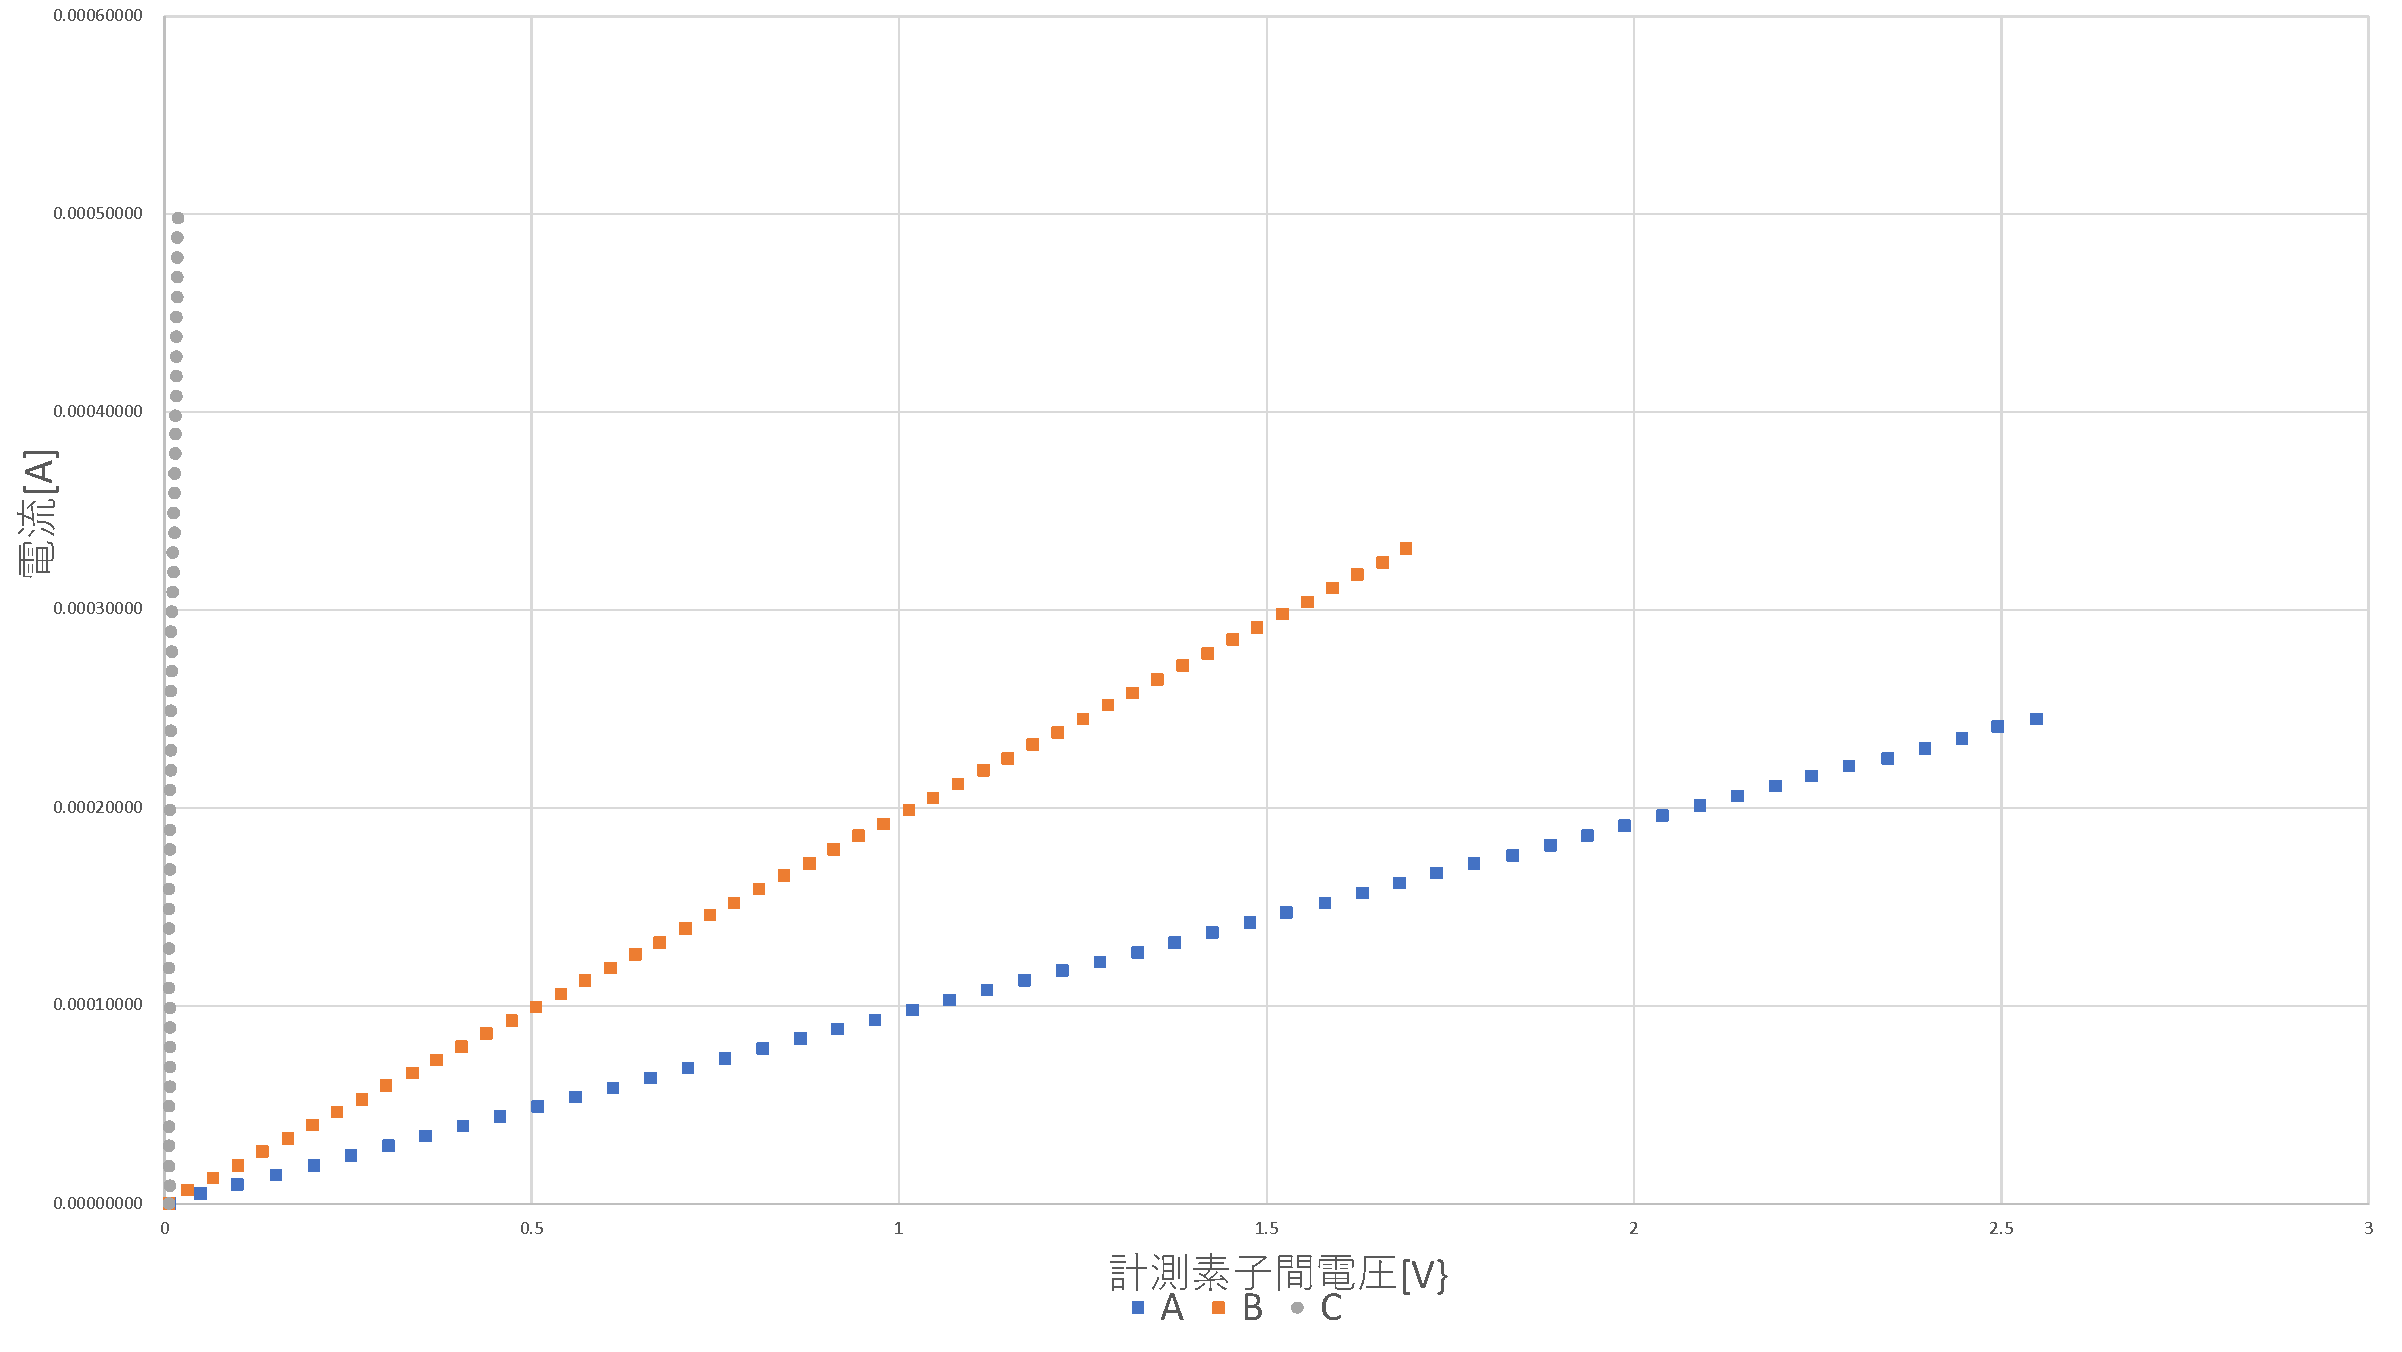
\includegraphics[scale=0.315]{./fig/3-2-1.pdf}}
	\caption{可変抵抗器(1-2端子間)の電圧電流特性}
	\label{fig:3-2-1}
	%\end{minipage}
  %\begin{minipage}[c]{0.5\hsize}
    \centering
   \subfloat{ 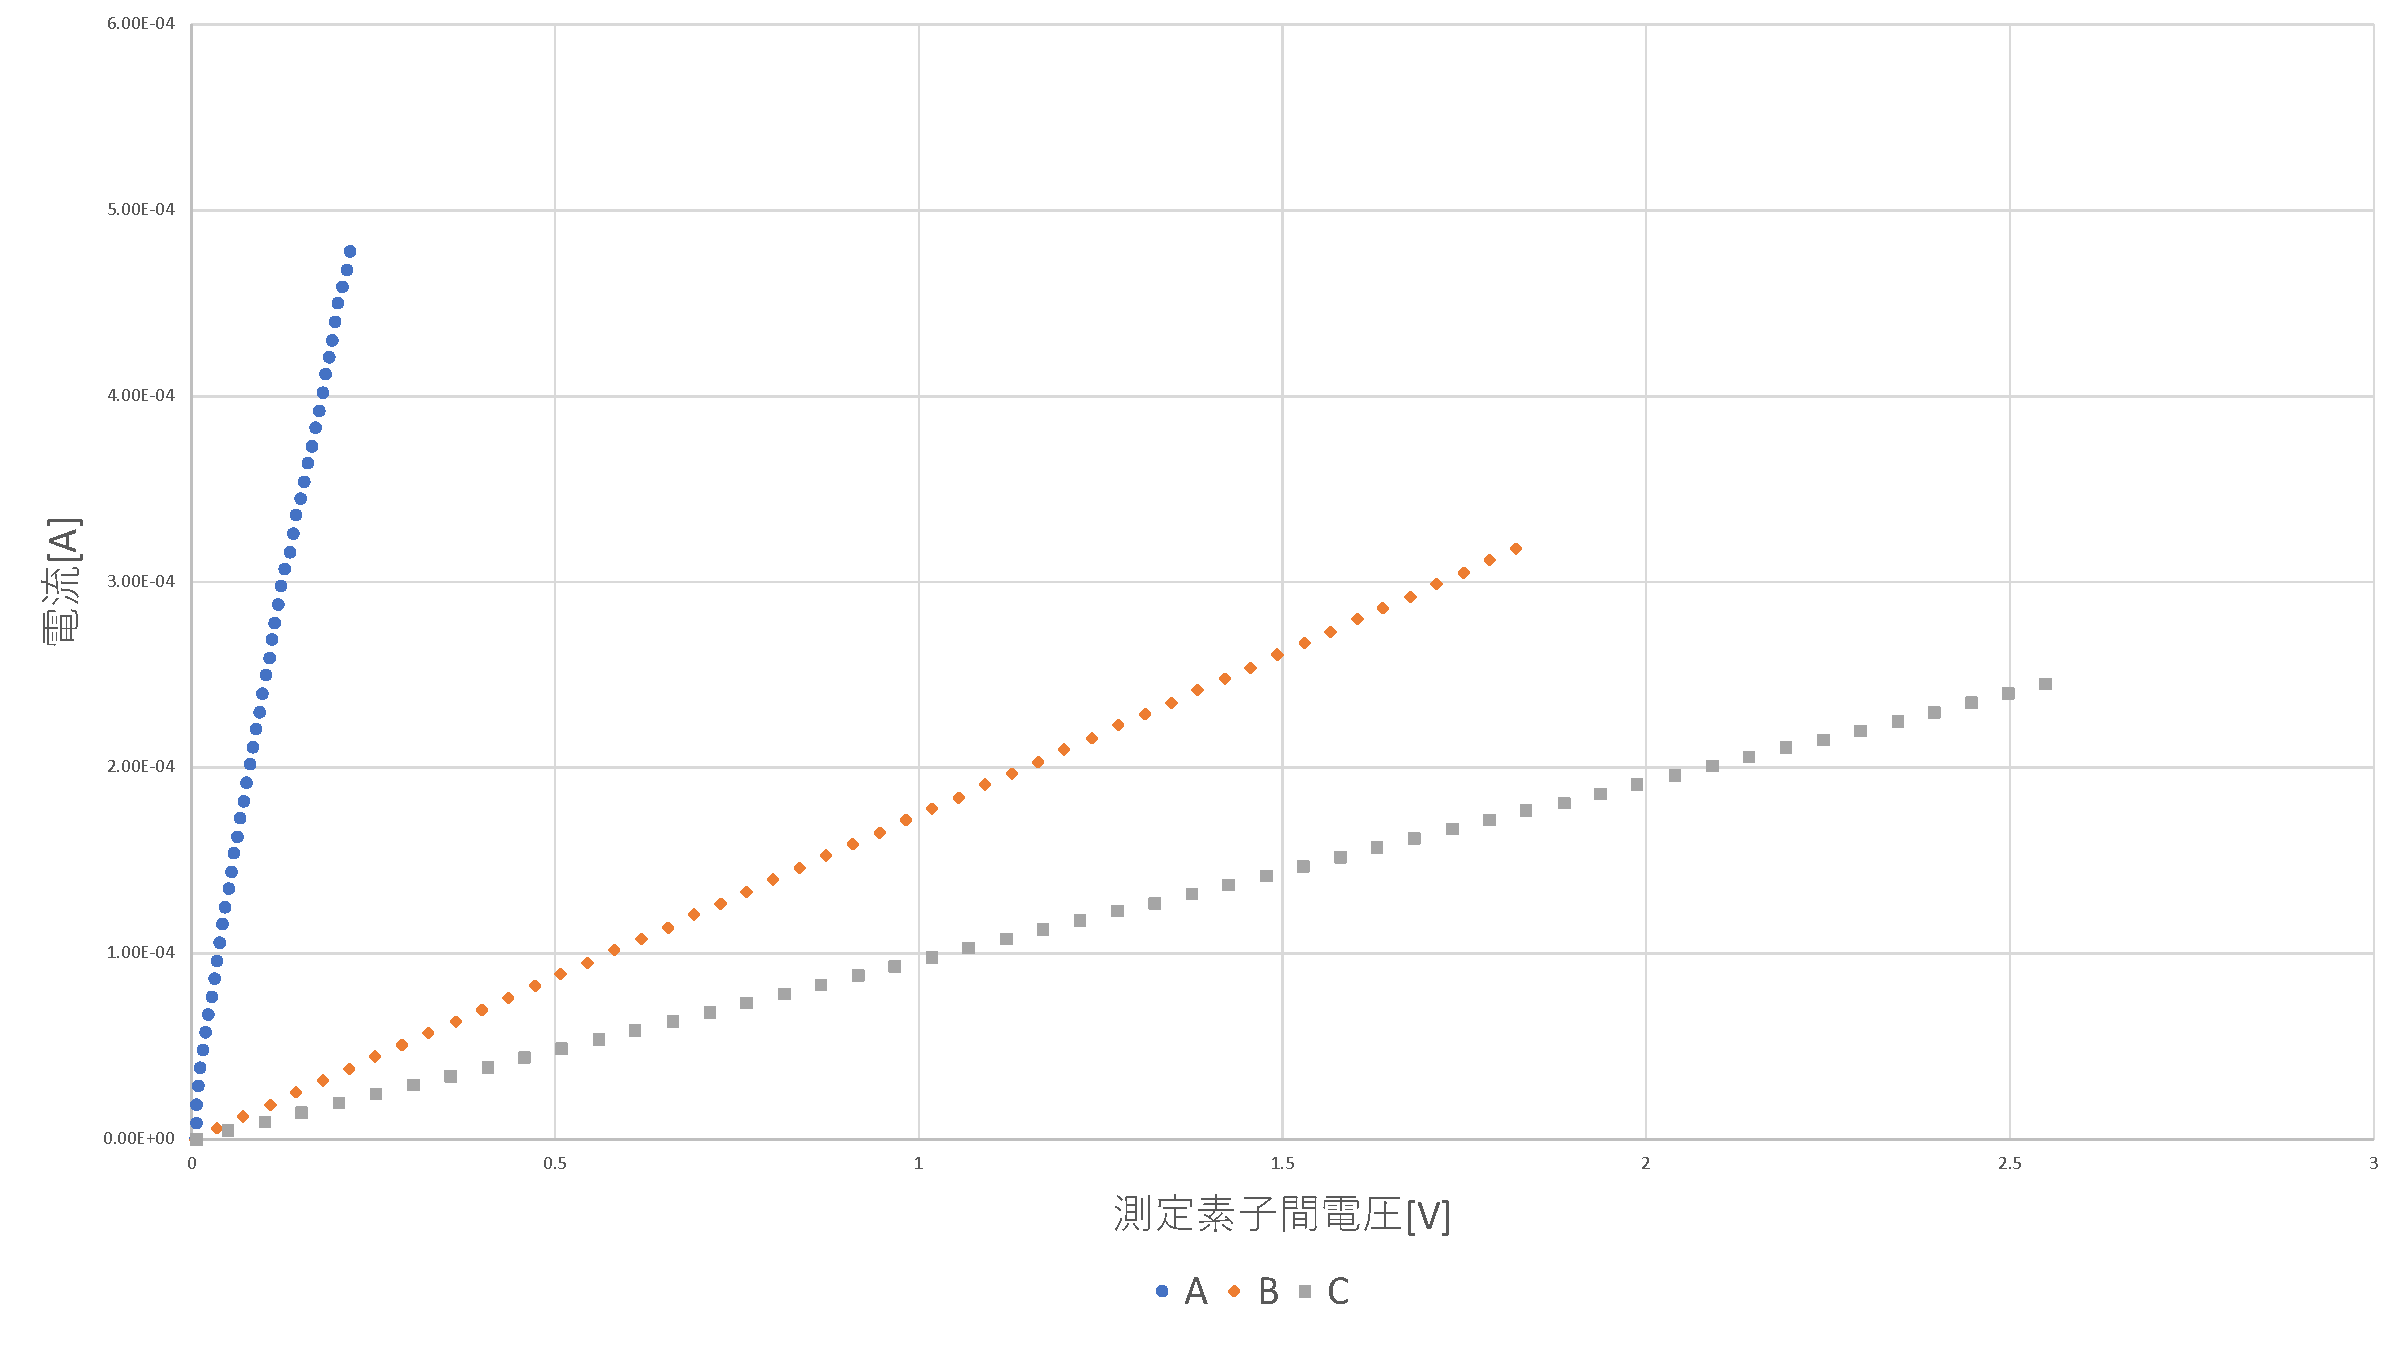
\includegraphics[scale=0.315]{./fig/3-2-2.pdf}}
	\caption{可変抵抗器(2-3端子間)の電圧電流特性}
	\label{fig:3-2-2}
  %\end{minipage}
  %\begin{minipage}[c]{0.5\hsize}
  \centering
  \centering
        \subfloat{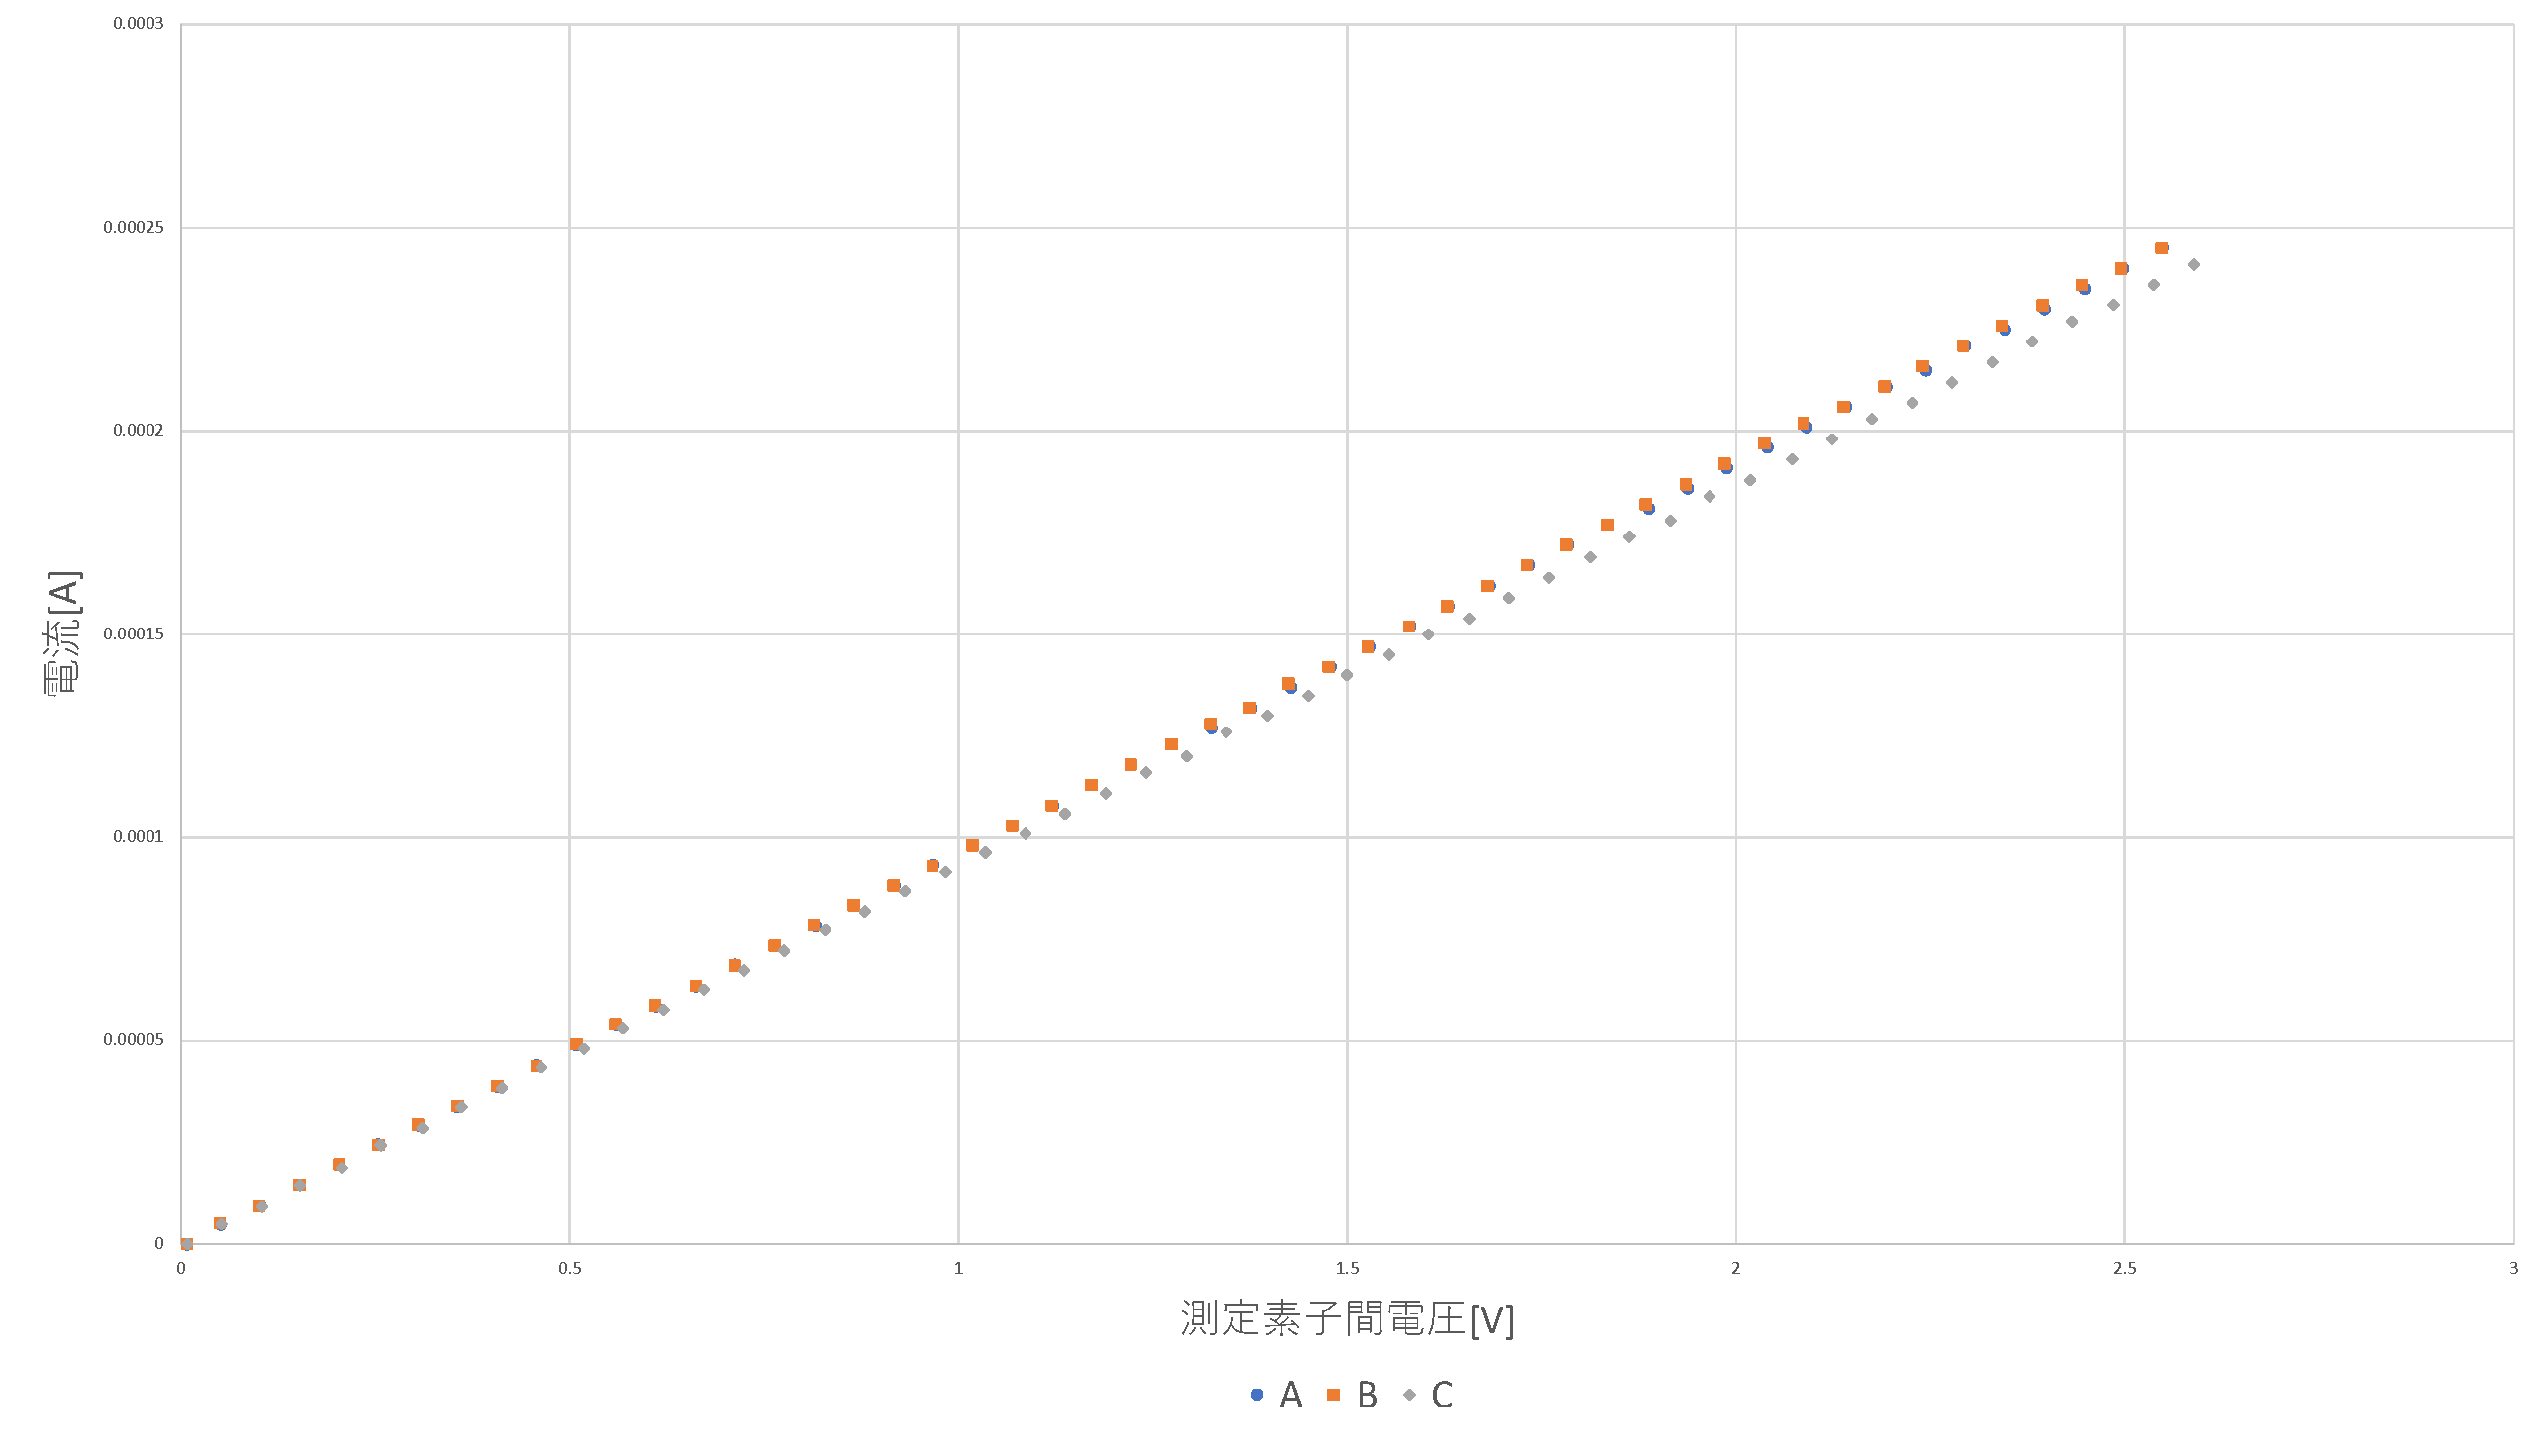
\includegraphics[scale=0.31]{./fig/3-2-3.pdf}}
	\caption{可変抵抗器(3-1端子間)の電圧電流特性}
	\label{fig:3-2-3}
 %\end{minipage}
\end{figure}
\clearpage
\subsection{実習3-3 CdSセンサの電圧電流特性}
\begin{itemize}
	\item プログラムは上記の\ref{ex32-block}と同じものを利用し,$R_{0}$の値は10\,k\rm{$\Omega$}とした.
	\item 実行後,フロントパネルは\wfig{ex33-flont}のようになり,計測結果は\wtab{CDS}のようになった.
	\item 計測データを基に作成した電圧電流特性のグラフは\wfig{3-3}である.
\end{itemize}

 \begin{figure}[h]
  \centering
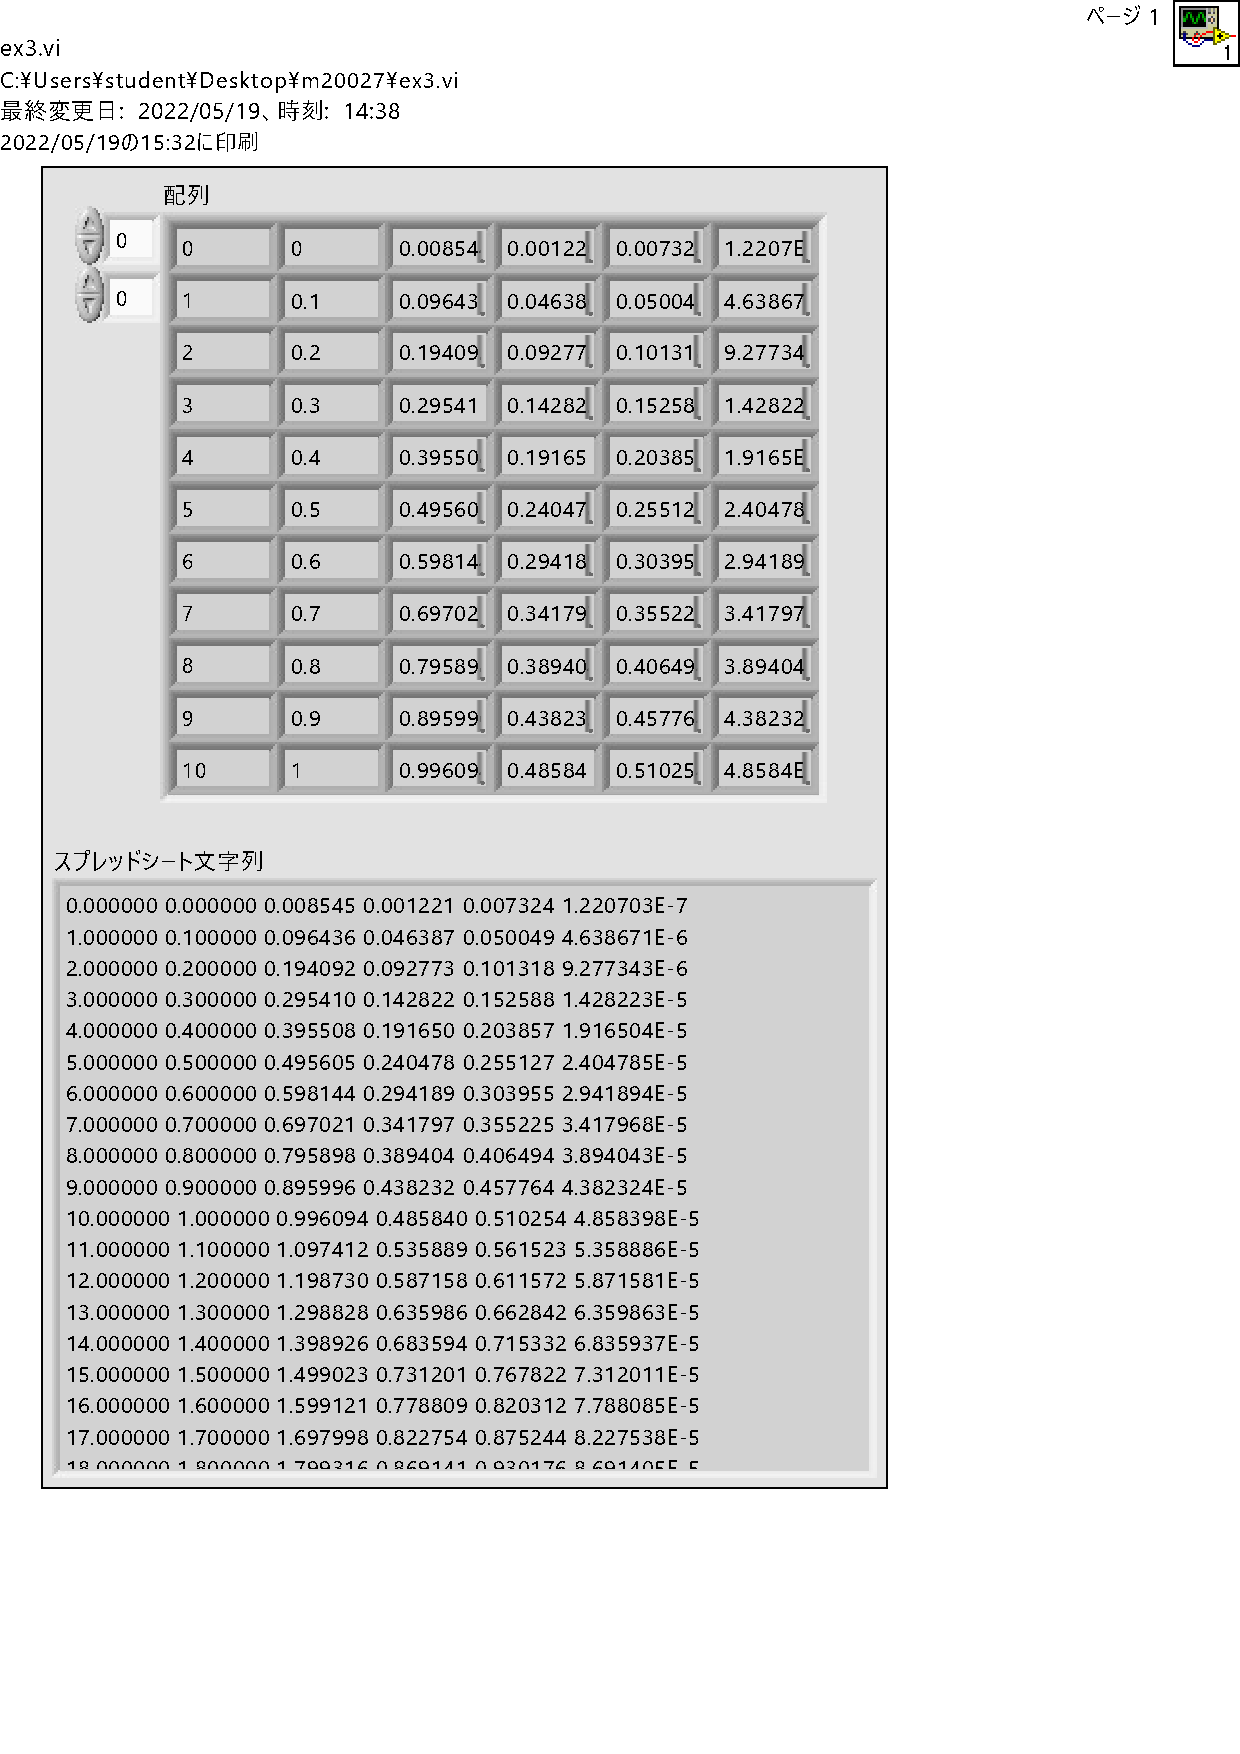
\includegraphics[scale=0.35]{./fig/ex33-flont.pdf}
\caption{CdSセンサの電圧電流特性測定時のフロントパネル}
\label{fig:ex33-flont}
\end{figure}

\begin{figure}[h]
\centering
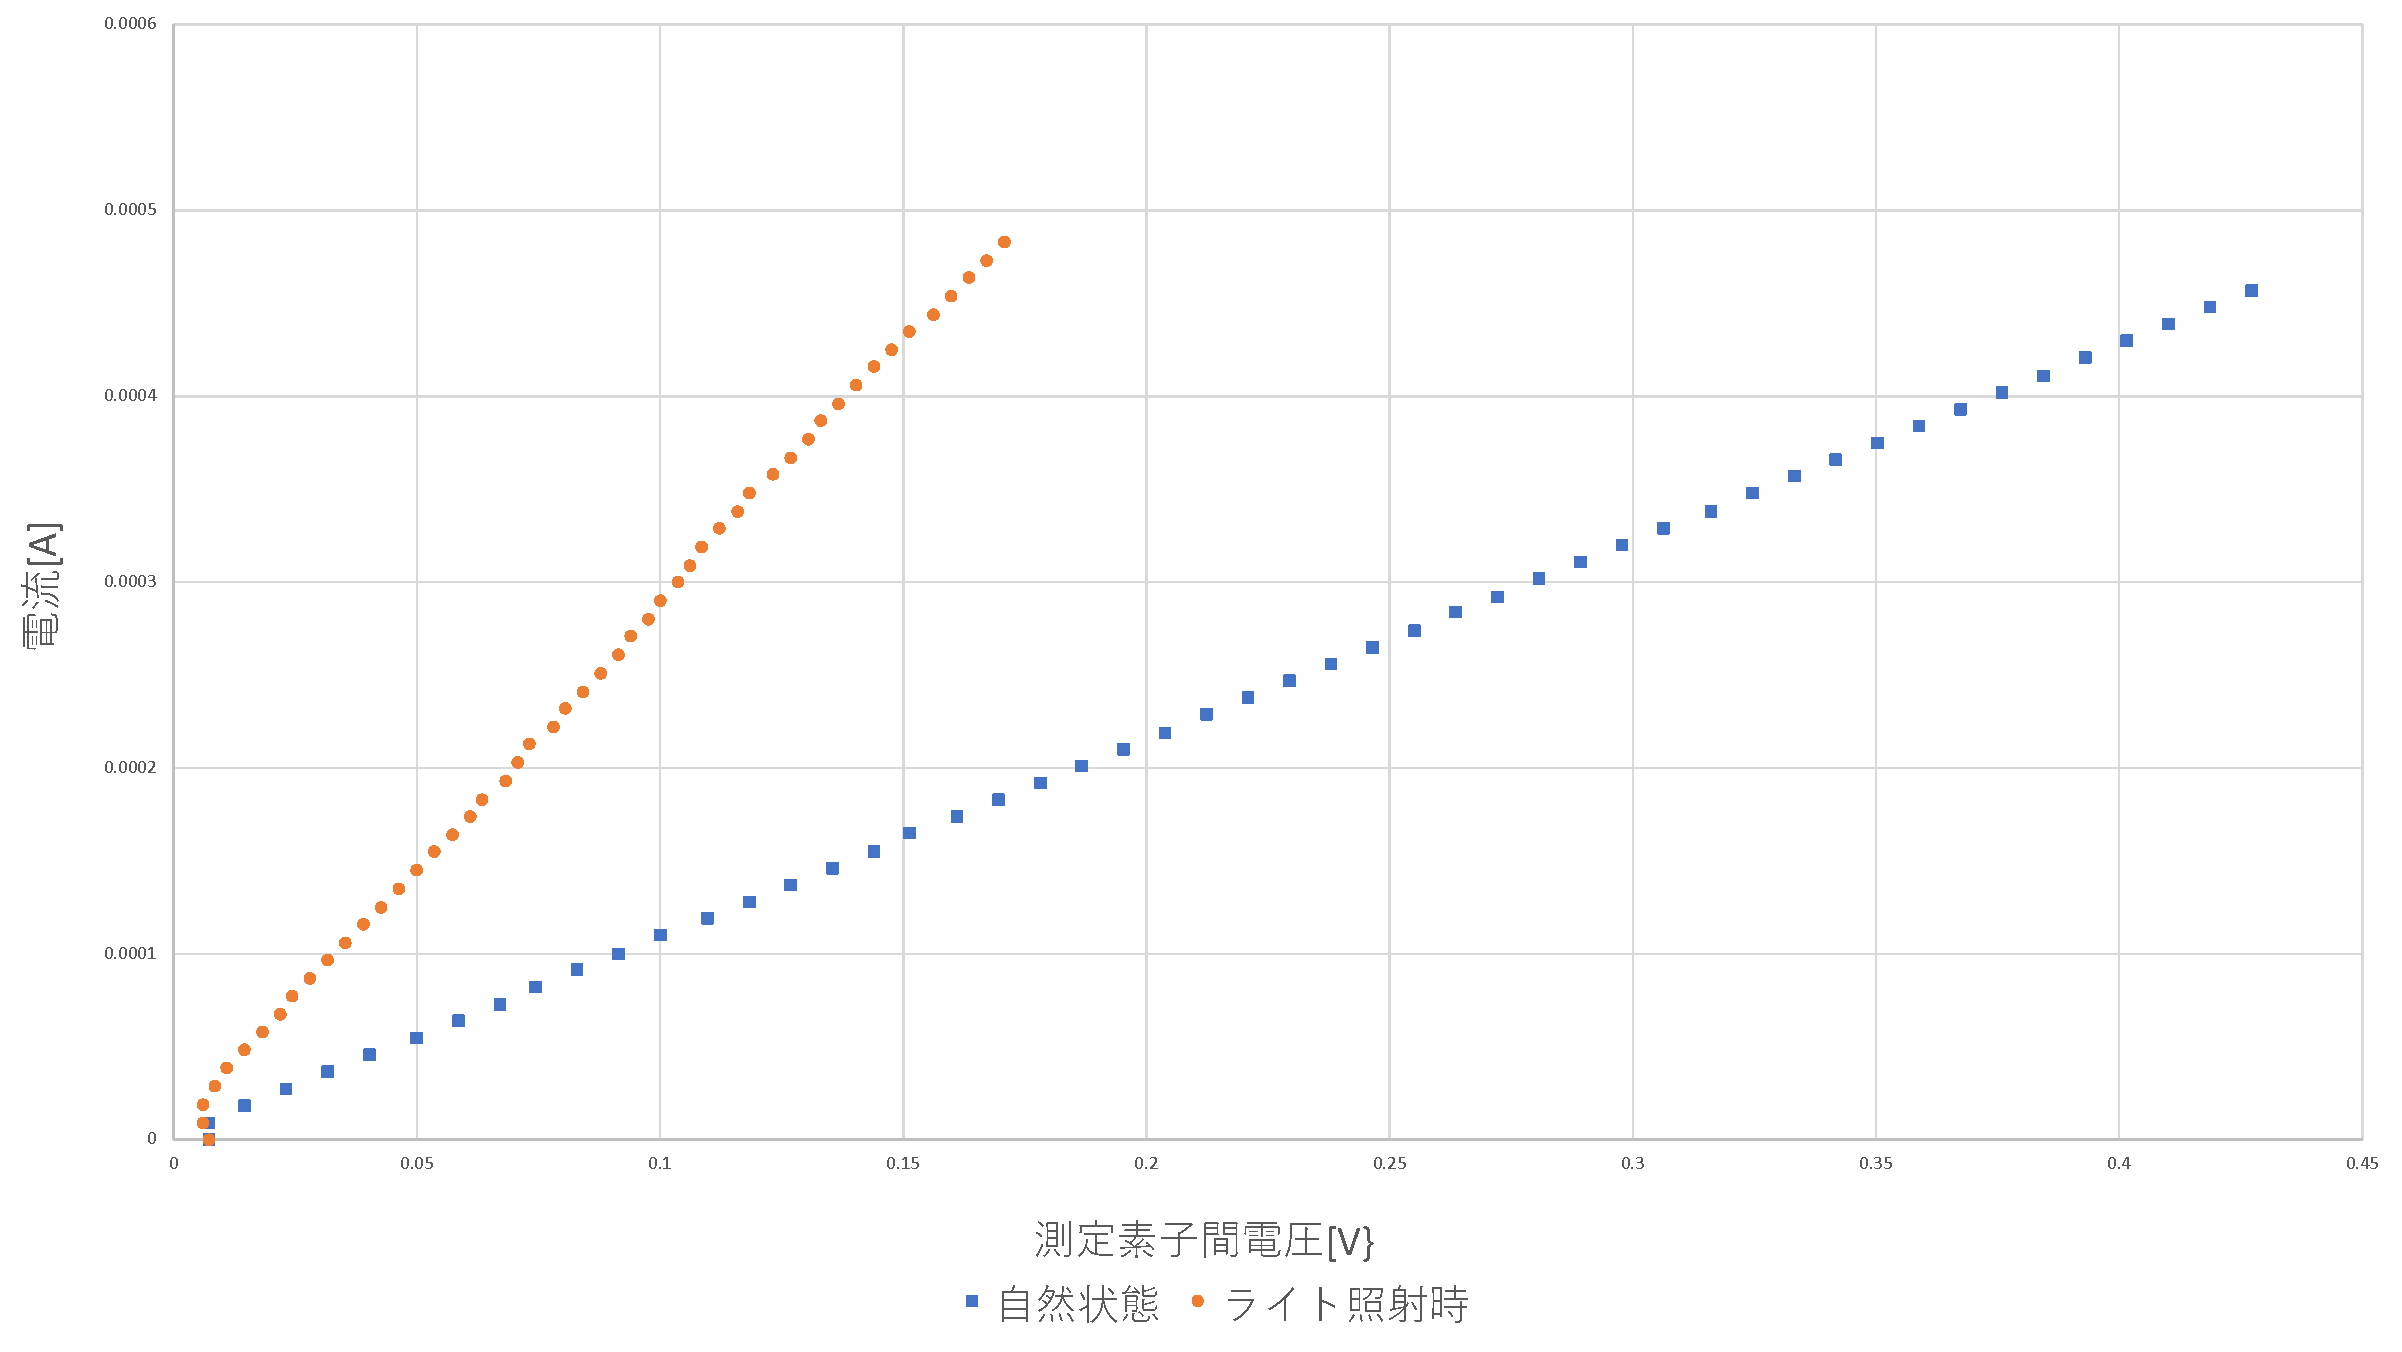
\includegraphics[scale=0.38]{./fig/3-3.pdf}
\caption{CdSセンサの電圧電流特性}
\label{fig:3-3}
\end{figure}

\begin{table}[h]
    \centering
    \caption{CdSセンサの諸特性値}
    \label{tab:CDS}
     \scalebox{0.7}{
    \begin{tabular}{ccccc}
    \hline
    カウンタ変数 & 自然状態での$V_{U}$[\rm{V}] & 自然状態での$I_{U}$[\rm{A}]  & ライト照射時の$V_{U}$[\rm{V}] &ライト照射時の$I_{U}$[\rm{V}]   \\
    \hline
0      & 0.007324 & 0        & 0.007324 & 0.0000000 \\
1      & 0.007324 & 0.000009 & 0.006104 & 0.0000092 \\
2      & 0.014648 & 0.000018 & 0.006104 & 0.0000189 \\
3      & 0.023193 & 0.000027 & 0.008545 & 0.0000289 \\
4      & 0.031738 & 0.000037 & 0.010986 & 0.0000387 \\
5      & 0.040283 & 0.000046 & 0.014648 & 0.0000483 \\
6      & 0.050049 & 0.000055 & 0.018311 & 0.0000580 \\
7      & 0.058594 & 0.000064 & 0.021973 & 0.0000675 \\
8      & 0.067139 & 0.000073 & 0.024414 & 0.0000774 \\
9      & 0.074463 & 0.000082 & 0.028076 & 0.0000868 \\
10     & 0.083008 & 0.000092 & 0.031738 & 0.0000966 \\
11     & 0.091553 & 0.0001   & 0.0354   & 0.0001060 \\
12     & 0.100098 & 0.00011  & 0.039062 & 0.0001160 \\
13     & 0.109863 & 0.000119 & 0.042725 & 0.0001250 \\
14     & 0.118408 & 0.000128 & 0.046387 & 0.0001350 \\
15     & 0.126953 & 0.000137 & 0.050049 & 0.0001450 \\
16     & 0.135498 & 0.000146 & 0.053711 & 0.0001550 \\
17     & 0.144043 & 0.000155 & 0.057373 & 0.0001640 \\
18     & 0.151367 & 0.000165 & 0.061035 & 0.0001740 \\
19     & 0.161133 & 0.000174 & 0.063477 & 0.0001830 \\
20     & 0.169678 & 0.000183 & 0.068359 & 0.0001930 \\
21     & 0.178223 & 0.000192 & 0.070801 & 0.0002030 \\
22     & 0.186768 & 0.000201 & 0.073242 & 0.0002130 \\
23     & 0.195312 & 0.00021  & 0.078125 & 0.0002220 \\
24     & 0.203857 & 0.000219 & 0.080566 & 0.0002320 \\
25     & 0.212402 & 0.000229 & 0.084229 & 0.0002410 \\
26     & 0.220947 & 0.000238 & 0.087891 & 0.0002510 \\
27     & 0.229492 & 0.000247 & 0.091553 & 0.0002610 \\
28     & 0.238037 & 0.000256 & 0.093994 & 0.0002710 \\
29     & 0.246582 & 0.000265 & 0.097656 & 0.0002800 \\
30     & 0.255127 & 0.000274 & 0.100098 & 0.0002900 \\
31     & 0.263672 & 0.000284 & 0.10376  & 0.0003000 \\
32     & 0.272217 & 0.000292 & 0.106201 & 0.0003090 \\
33     & 0.280762 & 0.000302 & 0.108643 & 0.0003190 \\
34     & 0.289307 & 0.000311 & 0.112305 & 0.0003290 \\
35     & 0.297852 & 0.00032  & 0.115967 & 0.0003380 \\
36     & 0.306396 & 0.000329 & 0.118408 & 0.0003480 \\
37     & 0.316162 & 0.000338 & 0.123291 & 0.0003580 \\
38     & 0.324707 & 0.000348 & 0.126953 & 0.0003670 \\
39     & 0.333252 & 0.000357 & 0.130615 & 0.0003770 \\
40     & 0.341797 & 0.000366 & 0.133057 & 0.0003870 \\
41     & 0.350342 & 0.000375 & 0.136719 & 0.0003960 \\
42     & 0.358887 & 0.000384 & 0.140381 & 0.0004060 \\
43     & 0.367432 & 0.000393 & 0.144043 & 0.0004160 \\
44     & 0.375977 & 0.000402 & 0.147705 & 0.0004250 \\
45     & 0.384521 & 0.000411 & 0.151367 & 0.0004350 \\
46     & 0.393066 & 0.000421 & 0.15625  & 0.0004440 \\
47     & 0.401611 & 0.00043  & 0.159912 & 0.0004540 \\
48     & 0.410156 & 0.000439 & 0.163574 & 0.0004640 \\
49     & 0.418701 & 0.000448 & 0.167236 & 0.0004730 \\
50     & 0.427246 & 0.000457 & 0.170898 & 0.0004830 \\
\hline
  \end{tabular}
  }
 \end{table}
\clearpage
\subsection{実習3-4 力センサの電圧電流特性}
\begin{itemize}
	\item プログラムは上記の\ref{ex32-block}と同じものを利用し,$R_{0}$の値は10\,k\rm{$\Omega$}とした.
	\item 計測結果は\wtab{PS}のようになった.
	\item 計測データを基に作成した電圧電流特性のグラフは\wfig{3-4}である.
\end{itemize}

\begin{table}[h]
  \centering
    \caption{力センサの諸特性値}
    \label{tab:PS}
     \scalebox{0.8}{
    \begin{tabular}{ccccc}
    \hline
    カウンタ変数 & 自然状態での$V_{U}$[\rm{V}] & 自然状態での$I_{U}$[\rm{A}]  & 圧力ありでの$V_{U}$[\rm{V}] &圧力ありでの$I_{U}$[\rm{A}] \\
    \hline
 0  & 0.007324 & 0.0000001  & 0.006104 & 0.000000122 \\
1  & 0.100098 & -0.0000001 & 0.019531 & 0.00000793 \\
2  & 0.198975 & 0.0000000  & 0.037842 & 0.0000157 \\
3  & 0.299072 & -0.0000002 & 0.058594 & 0.0000237 \\
4  & 0.397949 & -0.0000001 & 0.081787 & 0.0000316 \\
5  & 0.494385 & 0.0000005  & 0.102539 & 0.0000397 \\
6  & 0.593262 & 0.0000004  & 0.12085  & 0.0000477 \\
7  & 0.692139 & 0.0000005  & 0.136719 & 0.0000559 \\
8  & 0.789795 & 0.0000007  & 0.161133 & 0.0000636 \\
9  & 0.887451 & 0.0000011  & 0.177002 & 0.0000720 \\
10 & 0.987549 & 0.0000010  & 0.194092 & 0.0000804 \\
11 & 1.086426 & 0.0000011  & 0.218506 & 0.0000880 \\
12 & 1.185303 & 0.0000012  & 0.236816 & 0.0000959 \\
13 & 1.28418  & 0.0000015  & 0.253906 & 0.000104 \\
14 & 1.381836 & 0.0000015  & 0.269775 & 0.000113 \\
15 & 1.483154 & 0.0000016  & 0.289307 & 0.000121 \\
16 & 1.58081  & 0.0000017  & 0.307617 & 0.000129 \\
17 & 1.678467 & 0.0000020  & 0.323486 & 0.000137 \\
18 & 1.779785 & 0.0000020  & 0.343018 & 0.000146 \\
19 & 1.876221 & 0.0000022  & 0.357666 & 0.000154 \\
20 & 1.975097 & 0.0000022  & 0.371094 & 0.000163 \\
21 & 2.075195 & 0.0000022  & 0.396728 & 0.00017  \\
22 & 2.172851 & 0.0000026  & 0.411377 & 0.000179 \\
23 & 2.272949 & 0.0000026  & 0.428467 & 0.000187 \\
24 & 2.370605 & 0.0000027  & 0.445557 & 0.000195 \\
25 & 2.470703 & 0.0000028  & 0.461426 & 0.000204 \\
26 & 2.568359 & 0.0000031  & 0.482178 & 0.000212 \\
27 & 2.667236 & 0.0000033  & 0.496826 & 0.00022  \\
28 & 2.766113 & 0.0000033  & 0.511475 & 0.000229 \\
29 & 2.86499  & 0.0000035  & 0.531006 & 0.000237 \\
30 & 2.963867 & 0.0000035  & 0.540771 & 0.000246 \\
31 & 3.063965 & 0.0000035  & 0.552978 & 0.000255 \\
32 & 3.161621 & 0.0000038  & 0.562744 & 0.000263 \\
33 & 3.261718 & 0.0000038  & 0.579834 & 0.000272 \\
34 & 3.360595 & 0.0000039  & 0.5896   & 0.000281 \\
35 & 3.459472 & 0.0000042  & 0.609131 & 0.000289 \\
36 & 3.558349 & 0.0000042  & 0.625    & 0.000297 \\
37 & 3.658447 & 0.0000042  & 0.635986 & 0.000306 \\
38 & 3.757324 & 0.0000045  & 0.653076 & 0.000314 \\
39 & 3.85498  & 0.0000046  & 0.664062 & 0.000324 \\
40 & 3.953857 & 0.0000046  & 0.679932 & 0.000332 \\
41 & 4.053955 & 0.0000045  & 0.690918 & 0.000341 \\
42 & 4.152832 & 0.0000048  & 0.716553 & 0.000348 \\
43 & 4.252929 & 0.0000049  & 0.725098 & 0.000358 \\
44 & 4.348144 & 0.0000051  & 0.738525 & 0.000366 \\
45 & 4.449462 & 0.0000050  & 0.756836 & 0.000374 \\
46 & 4.547119 & 0.0000055  & 0.770264 & 0.000383 \\
47 & 4.644775 & 0.0000057  & 0.793457 & 0.000391 \\
48 & 4.744873 & 0.0000056  & 0.814209 & 0.000398 \\
49 & 4.846191 & 0.0000054  & 0.837402 & 0.000406 \\
50 & 4.942626 & 0.0000056  & 0.863037 & 0.000414 \\
\hline
\end{tabular}
}
\end{table}

\begin{figure}[h]
\centering
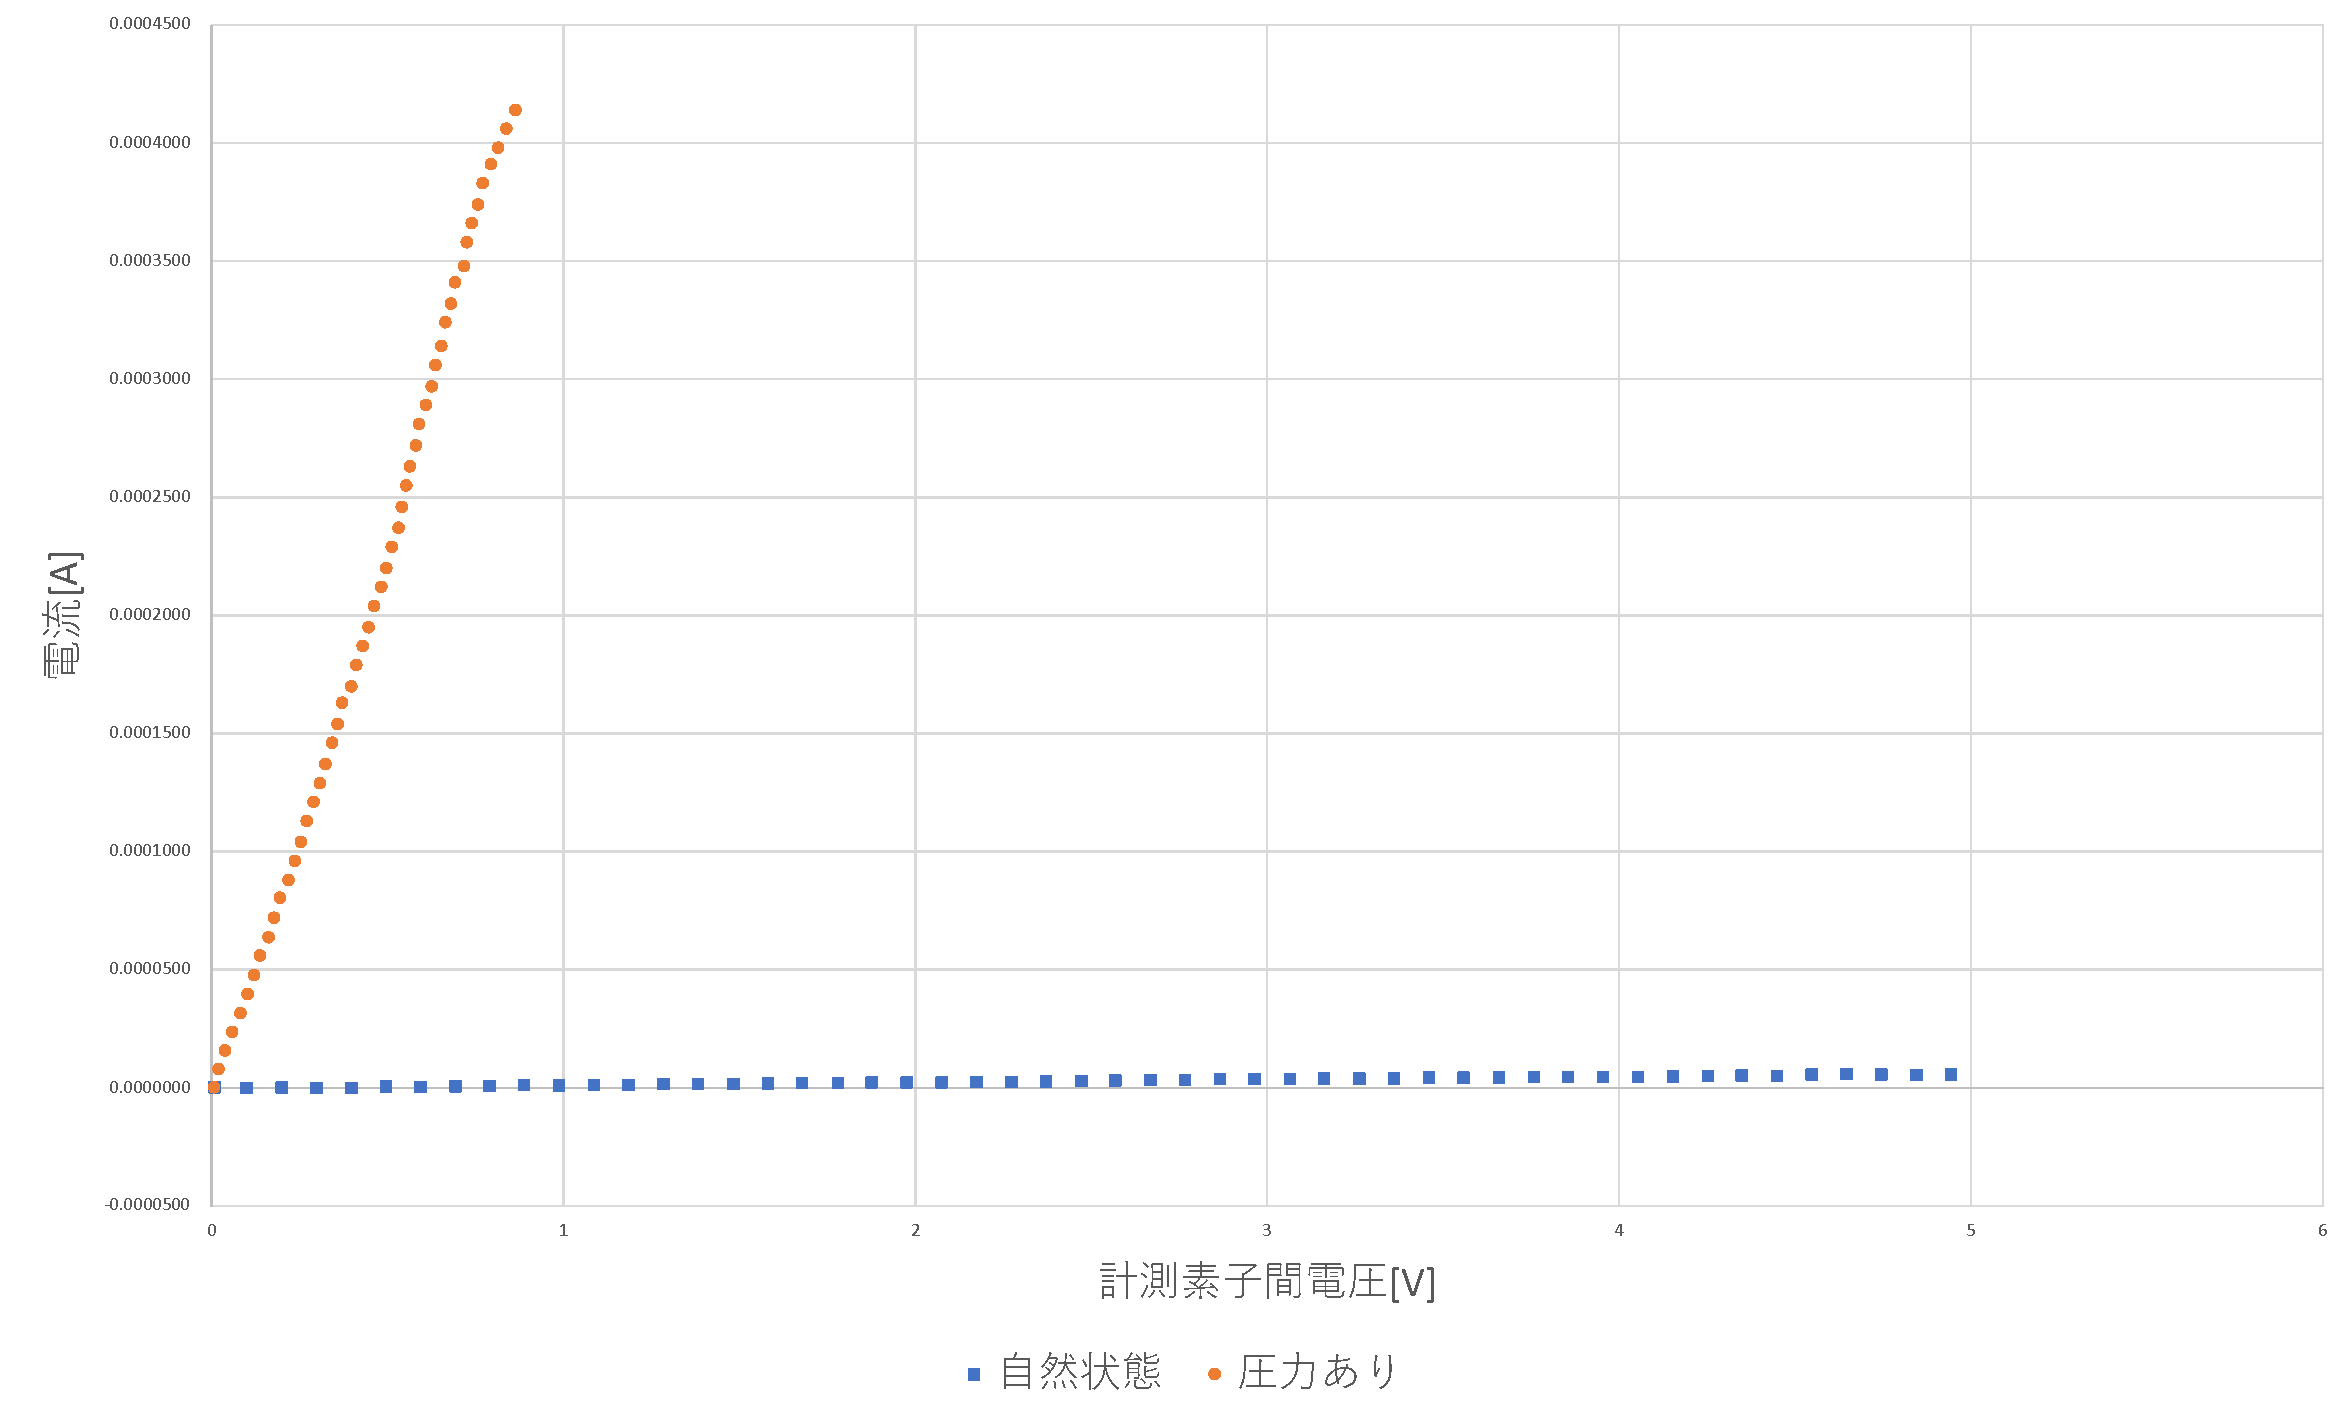
\includegraphics[scale=0.45]{./fig/3-4.pdf}
\caption{力センサの電圧電流特性}
\label{fig:3-4}
\end{figure}
\clearpage
\subsection{実習3-5 発光ダイオードの電圧電流特性}
\begin{itemize}
	\item プログラムは上記の\ref{ex32-block}と同じものを利用し,$R_{0}$の値は1\,k\rm{$\Omega$}とした.
	\item 計測結果は\wtab{LED}のようになった.
	\item 計測データを基に作成した電圧電流特性のグラフは\wfig{3-5}である.
\end{itemize}

\begin{table}[h]
\centering
\caption{LEDの諸特性値}
\label{tab:LED}
\scalebox{0.65}{
\begin{tabular}{ccccccccc}
\hline
ポインタ変数 & 赤色での$V_{U}$[\rm{V}]   & 赤色での$I_{U}$[\rm{A}]    & 青色での$V_{U}$[\rm{V}]      & 青色での$I_{U}$[\rm{A}]      & 白色での$V_{U}$[\rm{V}]    & 白色での$I_{U}$[\rm{A}]         & 緑色での$V_{U}$[\rm{V}]         & 緑色での$I_{U}$[\rm{A}]     \\
\hline
0      & 0.00732400 & 0.00000000  & 0.00732400 & 0.00000000  & 0.00610400 & 0.00000122 & 0.00610400 & 0.00000122  \\
1      & 0.09887700 & 0.00000366  & 0.09887700 & 0.00000366  & 0.09643600 & 0.00000732 & 0.09765600 & 0.00000610  \\
2      & 0.19775400 & 0.00000122  & 0.19531200 & 0.00000488  & 0.19653300 & 0.00000366 & 0.19897500 & -0.00000122 \\
3      & 0.29663100 & 0.00000122  & 0.29663100 & 0.00000122  & 0.29663100 & 0.00000244 & 0.29785200 & 0.00000000  \\
4      & 0.39672800 & 0.00000244  & 0.39917000 & -0.00000244 & 0.39672800 & 0.00000122 & 0.40039100 & -0.00000244 \\
5      & 0.49682600 & 0.00000244  & 0.49926800 & -0.00000122 & 0.49682600 & 0.00000244 & 0.49926800 & -0.00000122 \\
6      & 0.59570300 & 0.00000244  & 0.59936500 & -0.00000366 & 0.59692400 & 0.00000244 & 0.59570300 & 0.00000244  \\
7      & 0.69580100 & 0.00000244  & 0.69824200 & 0.00000000  & 0.69580100 & 0.00000244 & 0.69702100 & 0.00000122  \\
8      & 0.79589800 & 0.00000244  & 0.79589800 & 0.00000244  & 0.79711900 & 0.00000000 & 0.79834000 & -0.00000122 \\
9      & 0.89721700 & 0.00000122  & 0.89721700 & 0.00000244  & 0.89599600 & 0.00000244 & 0.89721700 & -0.00000122 \\
10     & 0.99609400 & 0.00000244  & 0.99731400 & -0.00000122 & 0.99487300 & 0.00000488 & 0.99853500 & -0.00000122 \\
11     & 1.09741200 & 0.00000000  & 1.09741200 & -0.00000122 & 1.09619100 & 0.00000244 & 1.09619100 & 0.00000122  \\
12     & 1.19751000 & 0.00000000  & 1.19873000 & -0.00000122 & 1.19506800 & 0.00000366 & 1.19873000 & -0.00000122 \\
13     & 1.29882800 & -0.00000122 & 1.29760700 & 0.00000000  & 1.29760700 & 0.00000122 & 1.29638700 & 0.00000122  \\
14     & 1.39770500 & 0.00000000  & 1.39648400 & 0.00000366  & 1.39648400 & 0.00000122 & 1.39770500 & 0.00000122  \\
15     & 1.49536100 & 0.00000122  & 1.49658200 & 0.00000122  & 1.49658200 & 0.00000244 & 1.49780300 & 0.00000000  \\
16     & 1.57959000 & 0.00001831  & 1.59545900 & 0.00000488  & 1.59668000 & 0.00000244 & 1.59668000 & 0.00000244  \\
17     & 1.63696300 & 0.00005981  & 1.69799800 & 0.00000000  & 1.69677700 & 0.00000122 & 1.69677700 & 0.00000244  \\
18     & 1.67602500 & 0.00012200  & 1.79687500 & 0.00000244  & 1.79809600 & 0.00000000 & 1.79687500 & 0.00000000  \\
19     & 1.70288100 & 0.00019400  & 1.89697200 & -0.00000122 & 1.89697200 & 0.00000000 & 1.89697200 & 0.00000122  \\
20     & 1.72485300 & 0.00027200  & 1.99462900 & 0.00000366  & 1.99584900 & 0.00000244 & 1.99584900 & 0.00000244  \\
21     & 1.74438500 & 0.00035300  & 2.09472600 & 0.00000488  & 2.09594700 & 0.00000244 & 2.09472600 & 0.00000488  \\
22     & 1.76025400 & 0.00043700  & 2.19604500 & 0.00000244  & 2.19604500 & 0.00000244 & 2.19604500 & 0.00000122  \\
23     & 1.77734400 & 0.00051900  & 2.29614200 & 0.00000244  & 2.29492200 & 0.00000366 & 2.29370100 & 0.00000488  \\
24     & 1.79077100 & 0.00060700  & 2.39135700 & 0.00000610  & 2.38769500 & 0.00001099 & 2.38403300 & 0.00001465  \\
25     & 1.80542000 & 0.00069100  & 2.47070300 & 0.00002686  & 2.45239200 & 0.00004639 & 2.45727500 & 0.00004150  \\
26     & 1.81762700 & 0.00077900  & 2.52807600 & 0.00007080  & 2.49145500 & 0.00010700 & 2.50854500 & 0.00009033  \\
27     & 1.83227500 & 0.00086700  & 2.56835900 & 0.00013200  & 2.51586900 & 0.00018300 & 2.54272400 & 0.00015600  \\
28     & 1.84326200 & 0.00095500  & 2.60009700 & 0.00019900  & 2.53295900 & 0.00026500 & 2.56835900 & 0.00022900  \\
29     & 1.85546900 & 0.00104100  & 2.62451100 & 0.00027500  & 2.54760700 & 0.00035000 & 2.58789000 & 0.00031000  \\
30     & 1.86767600 & 0.00112900  & 2.64648400 & 0.00035000  & 2.55981400 & 0.00043900 & 2.60498000 & 0.00039400  \\
31     & 1.87988300 & 0.00121700  & 2.66479500 & 0.00043300  & 2.56958000 & 0.00052900 & 2.61840800 & 0.00048100  \\
32     & 1.89209000 & 0.00130200  & 2.68066400 & 0.00051600  & 2.57812500 & 0.00062000 & 2.63183600 & 0.00056600  \\
33     & 1.90307600 & 0.00139300  & 2.69531200 & 0.00060200  & 2.58789000 & 0.00071000 & 2.64282200 & 0.00065600  \\
34     & 1.91406200 & 0.00148300  & 2.70874000 & 0.00068800  & 2.59399400 & 0.00080400 & 2.65258800 & 0.00074500  \\
35     & 1.92626900 & 0.00157100  & 2.72094700 & 0.00077600  & 2.60253900 & 0.00089600 & 2.66235300 & 0.00083600  \\
36     & 1.93725600 & 0.00165800  & 2.73315400 & 0.00086400  & 2.60986300 & 0.00098900 & 2.66967700 & 0.00092900  \\
37     & 1.94946300 & 0.00174600  & 2.74292000 & 0.00095500  & 2.61596700 & 0.00108300 & 2.67822200 & 0.00102100  \\
38     & 1.96044900 & 0.00183500  & 2.75268500 & 0.00104600  & 2.62207000 & 0.00117700 & 2.68676700 & 0.00111200  \\
39     & 1.97143500 & 0.00192400  & 2.76367200 & 0.00113500  & 2.62817400 & 0.00127100 & 2.69287100 & 0.00120600  \\
40     & 1.98242200 & 0.00201300  & 2.77343700 & 0.00122700  & 2.63305600 & 0.00136500 & 2.70019500 & 0.00129600  \\
41     & 1.99340800 & 0.00210200  & 2.78198200 & 0.00131600  & 2.63916000 & 0.00145900 & 2.70629900 & 0.00139200  \\
42     & 2.00561500 & 0.00219000  & 2.79052700 & 0.00140700  & 2.64404300 & 0.00155300 & 2.71362300 & 0.00148400  \\
43     & 2.01660100 & 0.00227800  & 2.79785100 & 0.00150100  & 2.65014600 & 0.00164700 & 2.71850600 & 0.00158000  \\
44     & 2.02636700 & 0.00236800  & 2.80639600 & 0.00159100  & 2.65502900 & 0.00174200 & 2.72460900 & 0.00167100  \\
45     & 2.03857400 & 0.00245500  & 2.81494100 & 0.00168200  & 2.65991200 & 0.00183600 & 2.73071300 & 0.00176600  \\
46     & 2.04956000 & 0.00254400  & 2.82226500 & 0.00177600  & 2.66479500 & 0.00193100 & 2.73559500 & 0.00186200  \\
47     & 2.06054700 & 0.00263400  & 2.82836900 & 0.00186800  & 2.66845700 & 0.00202600 & 2.74169900 & 0.00195400  \\
48     & 2.07275400 & 0.00272200  & 2.83691400 & 0.00195900  & 2.67456000 & 0.00212000 & 2.74658200 & 0.00205000  \\
49     & 2.08251900 & 0.00281000  & 2.84301700 & 0.00205400  & 2.67822200 & 0.00221800 & 2.75146500 & 0.00214600  \\
50     & 2.09350600 & 0.00289900  & 2.84912100 & 0.00214600  & 2.68310500 & 0.00231200 & 2.75634700 & 0.00224000  \\
\hline
\end{tabular}
}
\end{table}

\begin{figure}[h]
 \centering
        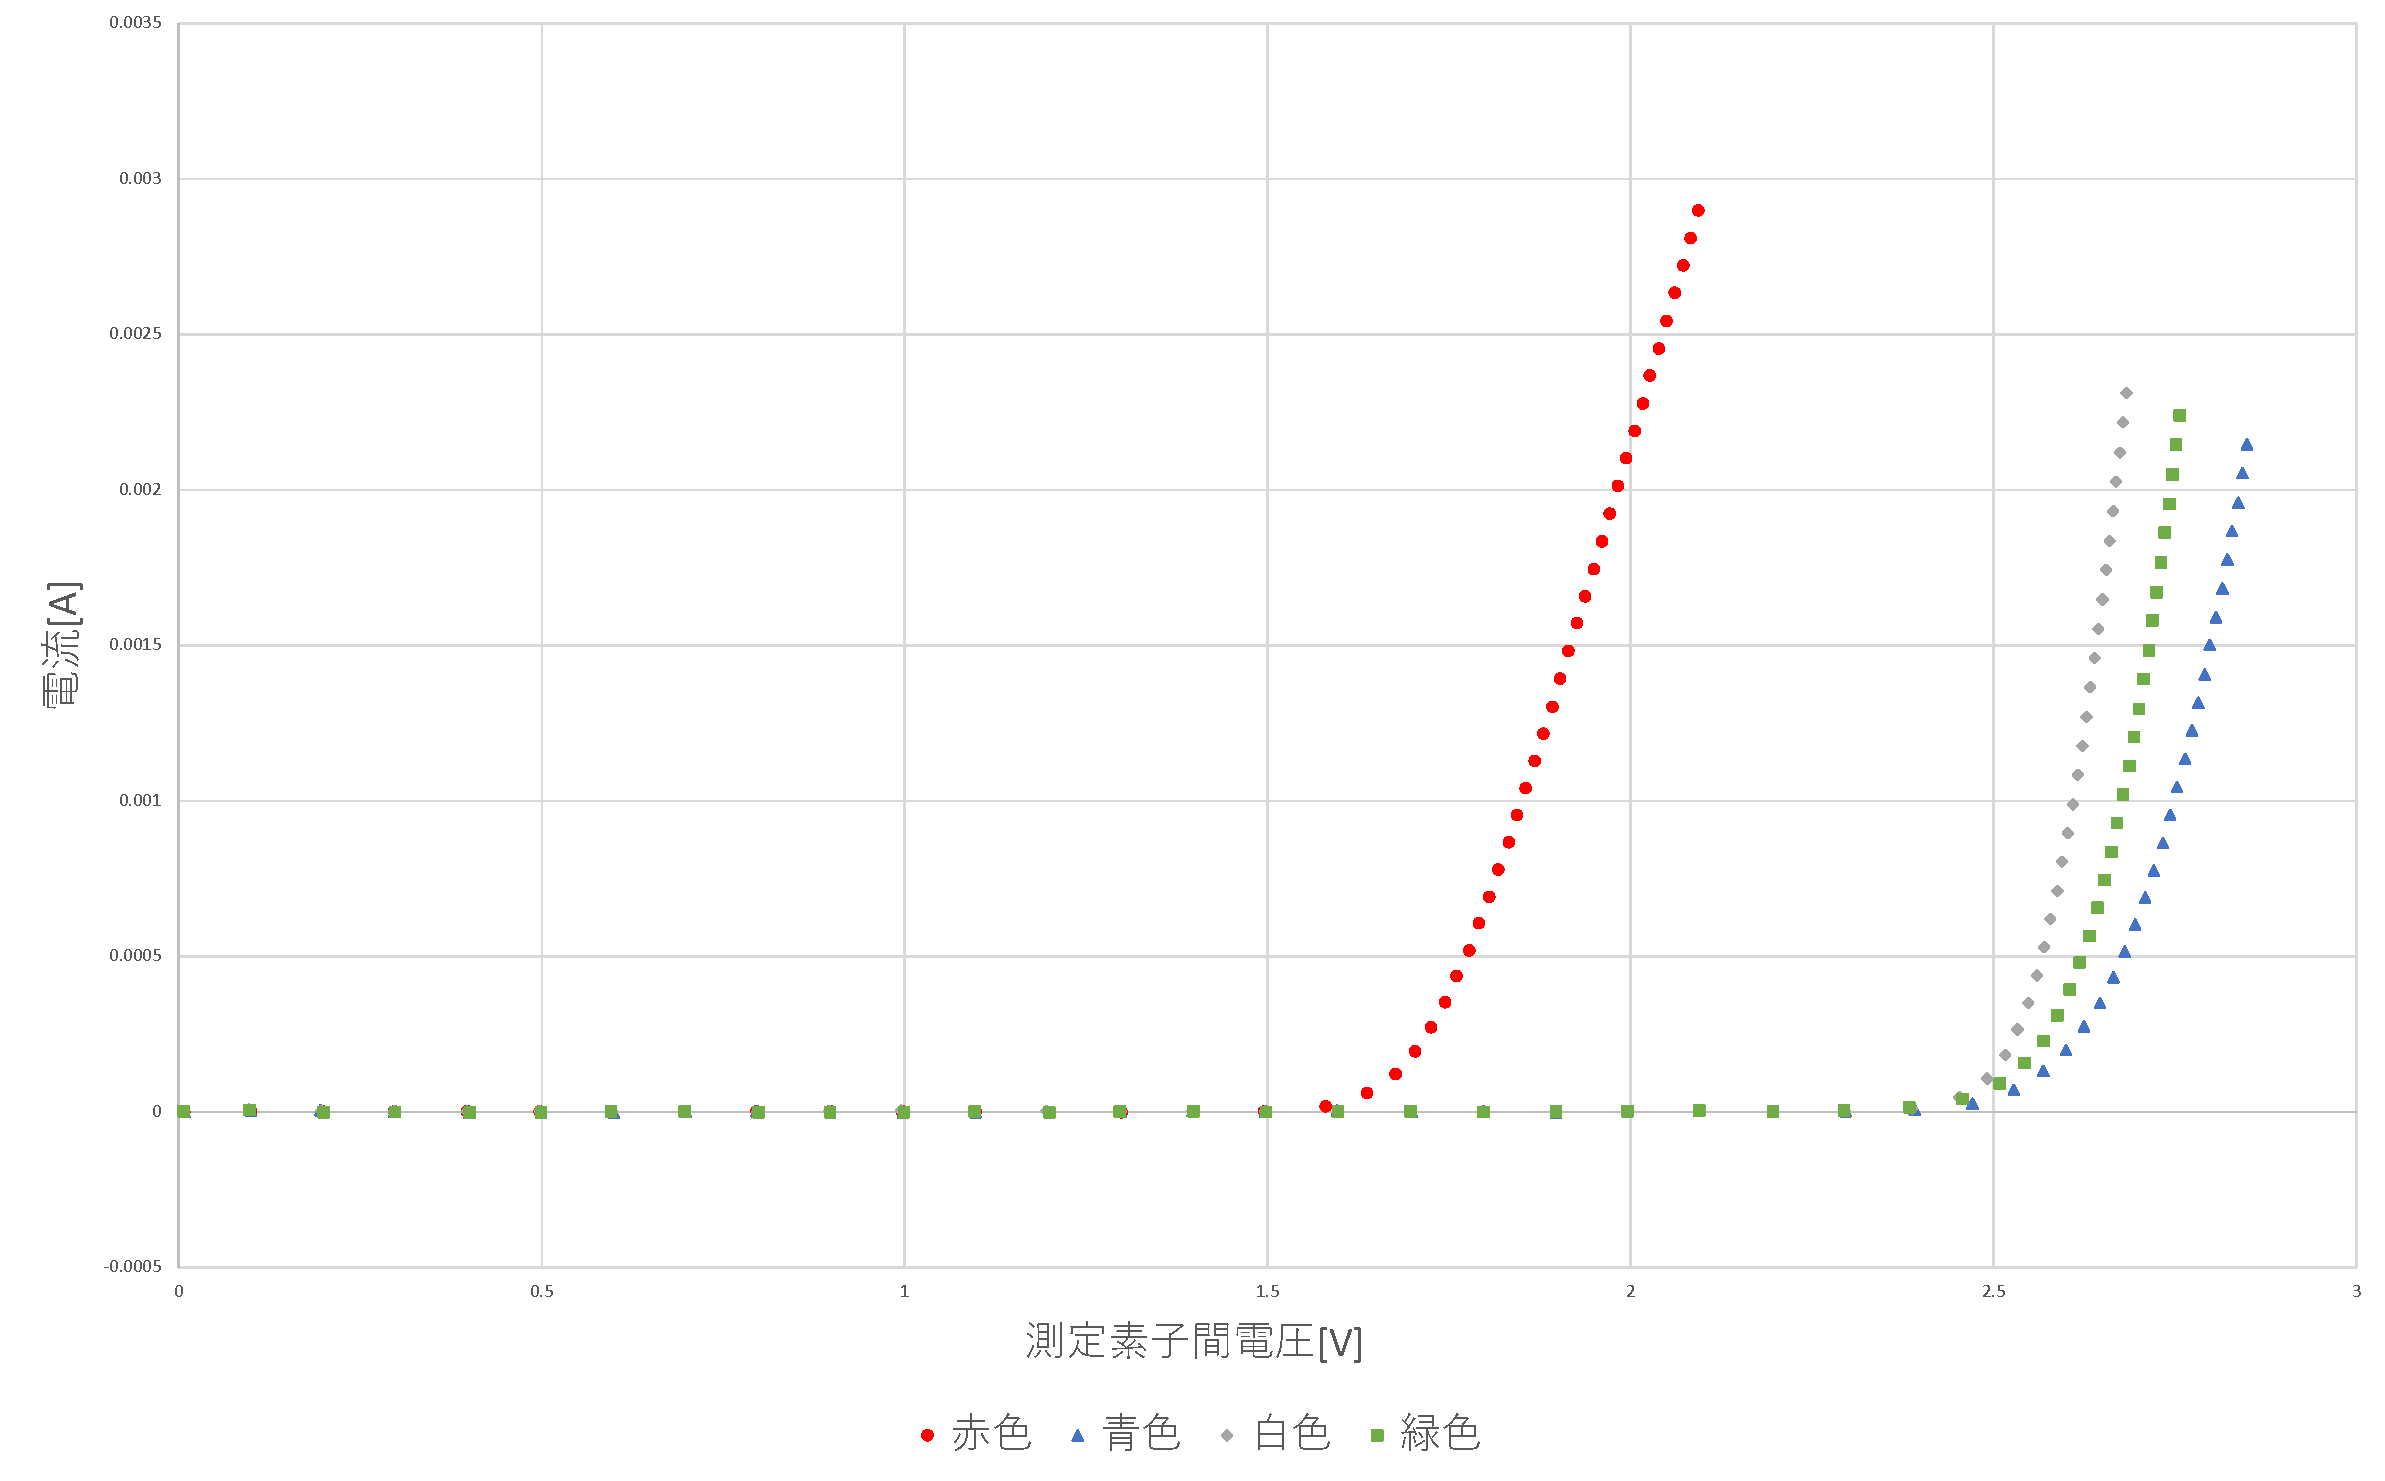
\includegraphics[scale=0.45]{./fig/3-5.pdf}
	\caption{LEDの電圧電流特性}
	\label{fig:3-5}
\end{figure}
\clearpage
\section{考察}
\begin{enumerate}[1.)]
	\item 各設定に対して,横軸が電流,縦軸が電力のグラフ(一つにまとめる)を描け.
	
	\wfig{L}に$X_{L}$での電流-電力特性を,\wfig{C}に$X_{C}$での電流-電力特性を示す.
	どちらの場合においても,力率が$1.0$に近づくほど全体的に多くの電力が得られていることがわかる.また,力率による電力への影響は電流が大きい場合であるほど大きくなっている.
	\begin{figure}[h]
	\centering
	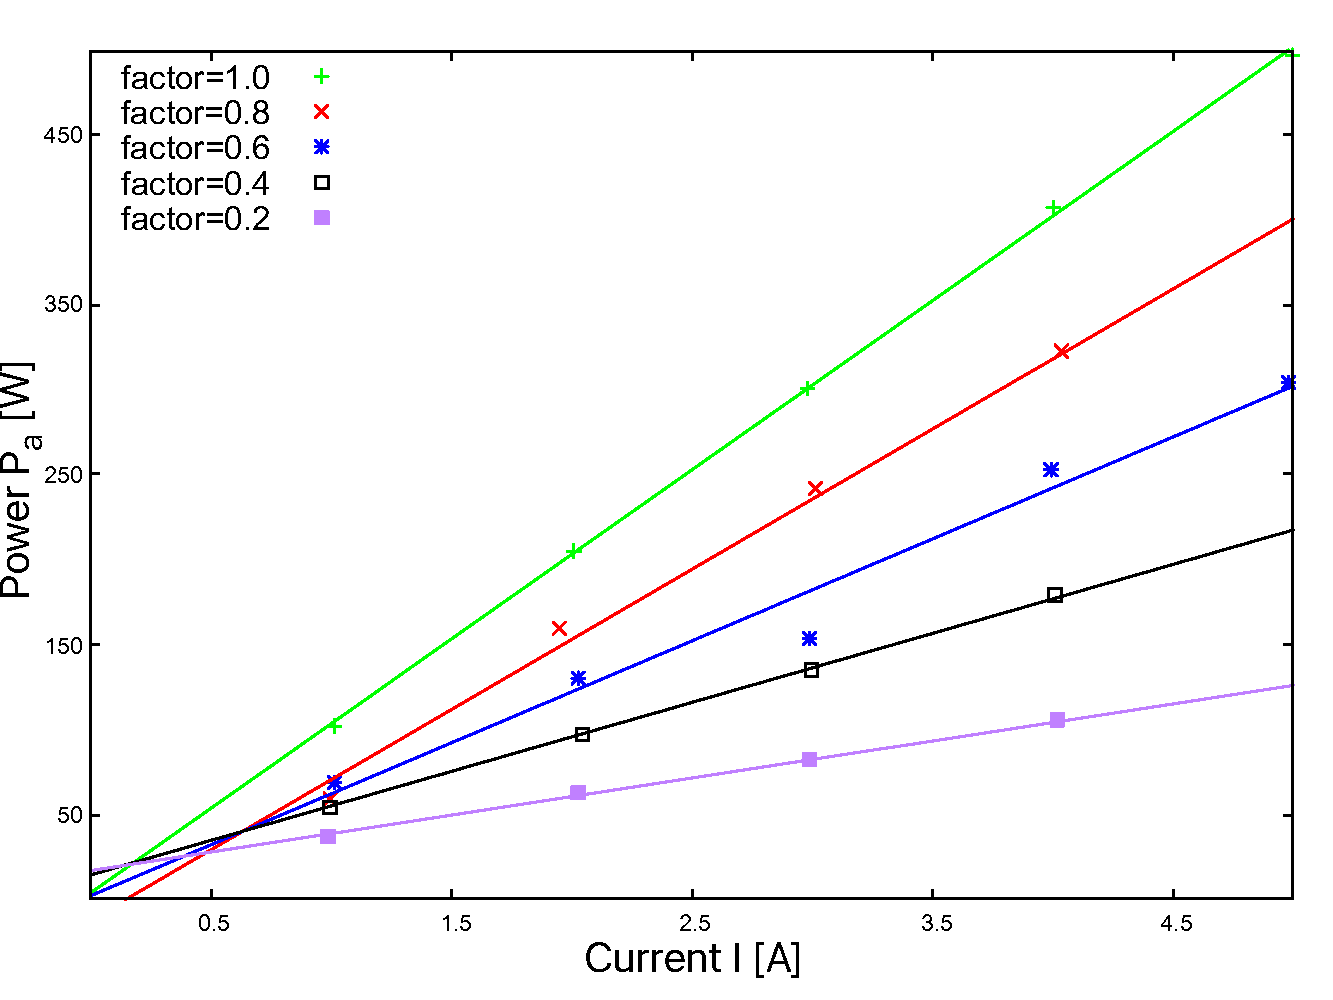
\includegraphics[scale=0.6]{./data/L/L.pdf}
	\caption{$X_L$の電流-電力特性}
	\label{fig:L}
	\end{figure}
	\begin{figure}[h]
	\centering
	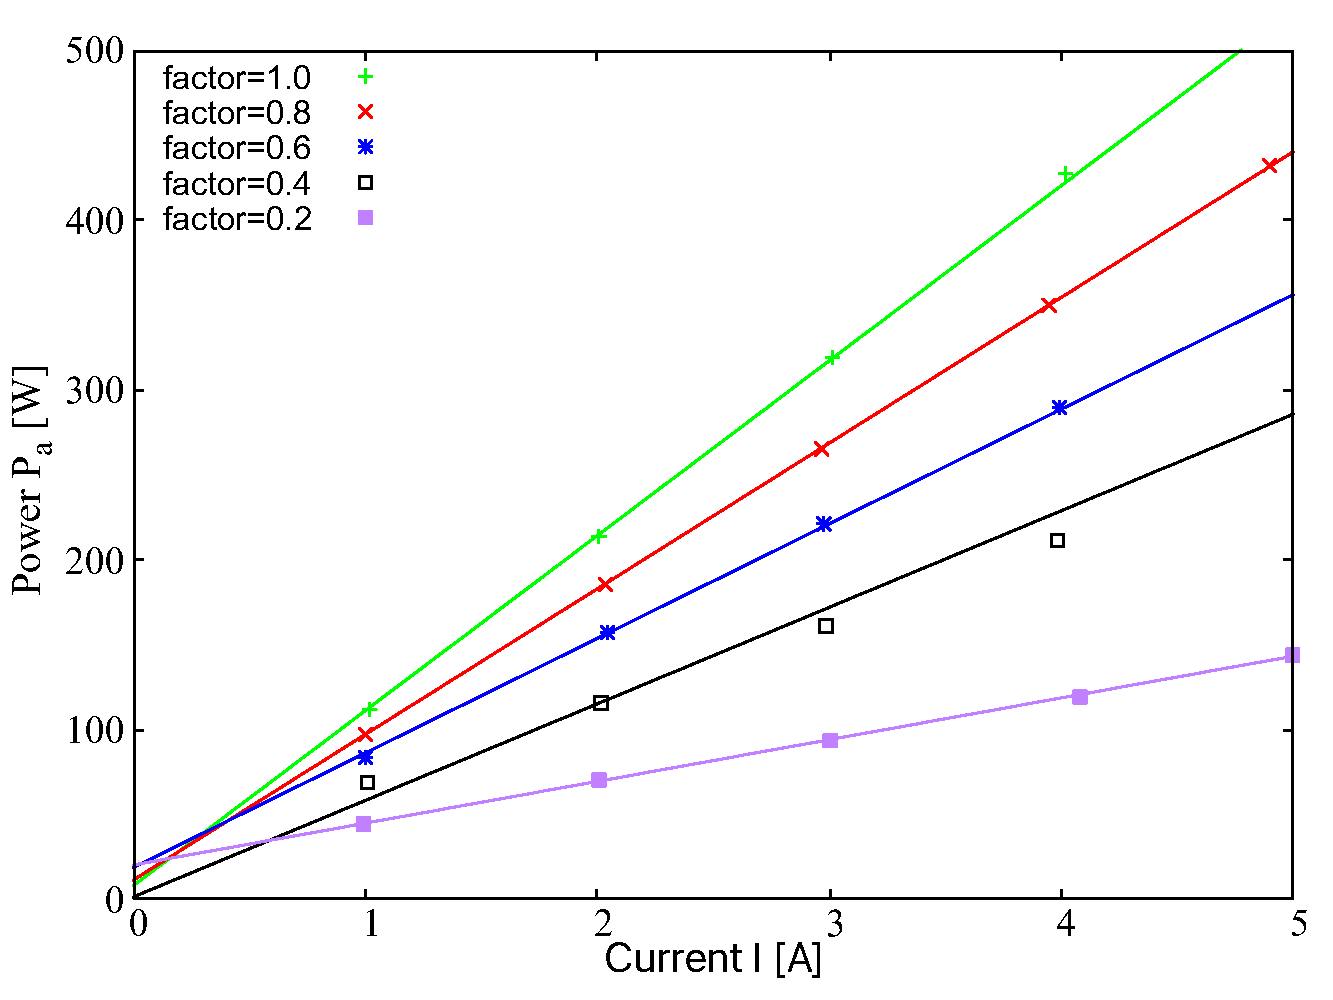
\includegraphics[scale=0.6]{./data/C/C.pdf}
	\caption{$X_C$の電流-電力特性}
	\label{fig:C}
	\end{figure}
	\item 各電流計の指示に対して,横軸が力率,縦軸が電力のグラフ(一つにまとめる)を描け.
	
	\wfig{},\wfig{}
	\item 電力と電圧,電流,力率の関係を述べよ.
	\item 
\end{enumerate}

\clearpage
\section{結論}
本実験を通して,
\begin{itemize}
	\item 自動計測の基礎をLabVIEWおよびMyRIOを使用して方法の習得.
	\item 最小二乗法などの近年でも有用な数値処理について計算方法の習得.
	\item 間接測定を利用した,測定データから抵抗値の導出.
	\item さまざまな素子の電流電圧特性の確認.
\end{itemize}
を達成することができた.

\newpage
\printbibliography[title=参考文献]
\end{document}
